\documentclass[11pt,a4paper,oneside]{report}

% Cargar paquetes
%\usepackage[utf8]{inputenc}
%\usepackage[T1]{fontenc}
\usepackage[spanish,es-tabla,es-noshorthands]{babel}
\usepackage{csquotes}                 


% GEOMETRÍA Y FORMATO
\usepackage[
    a4paper,
    left=2.5cm,
    right=2.5cm,
    top=3cm,
    bottom=3cm
]{geometry}

\setlength{\parindent}{0pt}
\setlength{\parskip}{0.5\baselineskip plus 2pt minus 1pt}     
\usepackage{setspace}
\setstretch{1.25}                     

\renewcommand{\thefootnote}{\roman{footnote}}  

% COLORES
\usepackage[dvipsnames,table,xcdraw]{xcolor}

% GRÁFICOS Y TABLAS
\usepackage{graphicx}
\usepackage{float}
\usepackage{caption}
\usepackage{subcaption}
\usepackage{booktabs}                 
\usepackage{array}
\usepackage{multirow}
\usepackage{tabularx}
\usepackage{xltabular}
\usepackage{makecell}
\usepackage{wrapfig} 
\usepackage{verbatim} 
\usepackage{comment}    
\usepackage{pgfgantt}    

\usepackage{array}

\newcolumntype{L}[1]{>{\raggedright\arraybackslash}p{#1}}
\newcolumntype{C}[1]{>{\centering\arraybackslash}p{#1}}
\newcolumntype{R}[1]{>{\raggedleft\arraybackslash}p{#1}}

% TIKZ Y DIAGRAMAS
\usepackage{tikz}                     % declaracion explicita (best practice)
\usepackage{pgfplots}
\pgfplotsset{compat=1.18}
\usetikzlibrary{
    positioning,                      % right=of, below=of, etc.
    arrows.meta,                      % puntas modernas (Stealth, Latex, etc.)
    shapes.geometric,                 % diamond, ellipse, trapezoid
    shapes.misc,                      % chamfered rectangle, etc.
    calc,                             % aritmetica de coordenadas ($(a)+(1,0)$)
    fit,                              % agrupar nodos en una caja
    backgrounds,                      % capas de fondo (\begin{scope}[on background layer])
    decorations.pathreplacing         % llaves y anotaciones sobre flechas
}


% Estilos comunes para diagramas (definidos UNA vez aqui, usados en todas las figuras)
\tikzset{
    block/.style={
        rectangle, draw, rounded corners=2pt,
        minimum height=9mm, minimum width=24mm,
        align=center, font=\small,
        inner sep=4pt
    },
    sensor/.style={
        block, fill=background_light
    },
    decision/.style={
        diamond, draw, aspect=2,
        align=center, font=\small,
        inner sep=1pt
    },
    terminal/.style={
        ellipse, draw, minimum width=20mm, minimum height=8mm,
        align=center, font=\small
    },
    arrow/.style={
        -Stealth, thick
    },
    bus/.style={
        -Stealth, very thick, double
    },
    label/.style={
        font=\scriptsize, midway, fill=white, inner sep=1pt
    }
}

% Colores personalizados
\definecolor{background_light}{RGB}{245,245,245}
\definecolor{border_color}{RGB}{120,120,120}
\definecolor{keyword_blue}{RGB}{0,0,180}
\definecolor{comment_green}{RGB}{34,139,34}
\definecolor{string_red}{RGB}{163,21,21}
\definecolor{number_gray}{RGB}{128,128,128}


% MATEMÁTICAS Y UNIDADES
\usepackage{amsmath,amsfonts,amssymb,amsthm}
\usepackage{textcomp}
\usepackage{gensymb}                 
\usepackage{siunitx}                  
\sisetup{
    output-decimal-marker={,},        
    per-mode=symbol,
    range-phrase={\,--\,},
    range-units=single,
    detect-all
}
% Definir unidades adicionales
\DeclareSIUnit\baud{Bd}
\DeclareSIUnit\sample{S}
\DeclareSIUnit{\eur}{\text{\euro}}

% LISTADOS DE CÓDIGO
\usepackage{listings}
\usepackage[framemethod=tikz]{mdframed}

% Marco para bloques de código
\mdfdefinestyle{CodeFrame}{
    roundcorner=5pt,
    backgroundcolor=background_light,
    linecolor=border_color,
    linewidth=0.5pt,
    innertopmargin=10pt,
    innerbottommargin=10pt,
    innerleftmargin=10pt,
    innerrightmargin=10pt,
    skipabove=10pt,
    skipbelow=10pt,
}

% Configuración base para código
\lstset{
    basicstyle=\ttfamily\small,
    breaklines=true,
    breakatwhitespace=false,
    columns=flexible,
    keepspaces=true,
    showstringspaces=false,
    showspaces=false,
    tabsize=4,
    frame=none,
    numbers=left,
    numberstyle=\tiny\color{number_gray},
    numbersep=8pt,
    xleftmargin=15pt,
    captionpos=b,
    extendedchars=true,
    inputencoding=utf8,
    literate=
        {á}{{\'a}}1 {é}{{\'e}}1 {í}{{\'i}}1 {ó}{{\'o}}1 {ú}{{\'u}}1
        {Á}{{\'A}}1 {É}{{\'E}}1 {Í}{{\'I}}1 {Ó}{{\'O}}1 {Ú}{{\'U}}1
        {ñ}{{\~n}}1 {Ñ}{{\~N}}1 {ü}{{\"u}}1 {Ü}{{\"U}}1,
}

% Estilo Arduino/C++ (para firmware ESP32)
\lstdefinestyle{Arduino}{
    language=C++,
    keywordstyle=\color{keyword_blue}\bfseries,
    commentstyle=\color{comment_green}\itshape,
    stringstyle=\color{string_red},
    morekeywords={
        HIGH,LOW,INPUT,OUTPUT,INPUT_PULLUP,LED_BUILTIN,
        Serial,Wire,String,boolean,byte,word,
        pinMode,digitalWrite,digitalRead,analogRead,analogWrite,
        delay,millis,micros,setup,loop,
        Serial1,Serial2,HardwareSerial,BluetoothSerial,
        begin,print,println,available,read,write,flush,
        uint8_t,uint16_t,uint32_t,int8_t,int16_t,int32_t,
        float,double,void,bool,true,false,NULL,
        PROGMEM,F,sizeof,static_cast
    },
    morecomment=[l]{//},
    morecomment=[s]{/*}{*/},
    morestring=[b]",
    morestring=[b]',
}

% Estilo Processing/Java (para software PFD)
\lstdefinestyle{Processing}{
    language=Java,
    keywordstyle=\color{keyword_blue}\bfseries,
    commentstyle=\color{comment_green}\itshape,
    stringstyle=\color{string_red},
    morekeywords={
        void,setup,draw,settings,size,fullScreen,
        background,fill,stroke,noFill,noStroke,strokeWeight,
        ellipse,rect,line,arc,triangle,quad,point,vertex,
        beginShape,endShape,curveVertex,bezierVertex,
        translate,rotate,scale,pushMatrix,popMatrix,resetMatrix,
        color,loadImage,image,PImage,PFont,textFont,createFont,
        text,textSize,textAlign,textWidth,
        mouseX,mouseY,mousePressed,keyPressed,key,keyCode,
        width,height,frameRate,frameCount,displayWidth,displayHeight,
        Serial,printArray,println,print,nf,nfc,nfp,nfs,
        map,constrain,lerp,norm,dist,mag,
        radians,degrees,sin,cos,tan,atan2,asin,acos,
        sqrt,pow,abs,min,max,floor,ceil,round,
        random,noise,randomSeed,noiseSeed,
        CENTER,LEFT,RIGHT,TOP,BOTTOM,CORNER,CORNERS,BASELINE,
        PI,TWO_PI,HALF_PI,QUARTER_PI,TAU,
        RGB,HSB,ARGB,ALPHA,
        CLOSE,OPEN,CHORD,PIE
    },
    morecomment=[l]{//},
    morecomment=[s]{/*}{*/},
}

% Estilo Python
\lstdefinestyle{Python}{
    language=Python,
    keywordstyle=\color{keyword_blue}\bfseries,
    commentstyle=\color{comment_green}\itshape,
    stringstyle=\color{string_red},
    morekeywords={self,True,False,None,as,with,lambda,yield,async,await},
}

% Nombre de los listados en español
\renewcommand{\lstlistingname}{Código}
\renewcommand{\lstlistlistingname}{Índice de Códigos}


% LISTAS Y ENUMERACIÓN
\usepackage{enumitem}


% ENCABEZADOS Y PIES DE PÁGINA
\usepackage{fancyhdr}
\setlength{\headheight}{15pt}
\setlength{\headsep}{0.5cm}

\pagestyle{fancy}
\fancyhf{} 

% Estilo para páginas normales
\fancyhead[L]{\small\leftmark}                    
\fancyhead[R]{\thepage} 
\renewcommand{\headrulewidth}{0.4pt}
\renewcommand{\footrulewidth}{0pt}

% Estilo para páginas de inicio de capítulo
\fancypagestyle{plain}{
    \fancyhf{}
    \fancyfoot[C]{\thepage}
    \renewcommand{\headrulewidth}{0pt}
}


% BIBLIOGRAFÍA
% BIBLIOGRAFIA (UNE-ISO 690, sistema numerico)
\usepackage[
    backend=biber,
    style=iso-numeric,      % <-- biblatex-iso690: implementa UNE-ISO 690
    sorting=none,           % orden de aparicion en el texto
    maxnames=3,
    minnames=1,
    shortnumeration=true,   % edicion abreviada: "3.a ed." en vez de "tercera edicion"
    pagetotal=false,        % no mostrar total de paginas
]{biblatex}

\addbibresource{../Common/references.bib}


% HIPERVÍNCULOS 
\usepackage{xurl}                     
\usepackage[
    colorlinks=true,
    linkcolor=black,
    urlcolor=blue,
    citecolor=blue,
    breaklinks=true,
    pdfauthor={Arnau},
    pdftitle={Flight Instruments Emulation Platform},
    pdfsubject={TFG - Trabajo de Fin de Grado},
    pdfkeywords={ESP32, IMU, GPS, PFD, instrumentación aérea},
    bookmarks=true,
    bookmarksnumbered=true
]{hyperref}


% REFERENCIAS CRUZADAS
\usepackage[spanish,capitalise]{cleveref}

% Personalizar nombres
\crefname{figure}{Figura}{Figuras}
\crefname{table}{Tabla}{Tablas}
\crefname{equation}{Ecuación}{Ecuaciones}
\crefname{chapter}{Capítulo}{Capítulos}
\crefname{section}{Sección}{Secciones}
\crefname{appendix}{Apéndice}{Apéndices}
\crefname{listing}{Código}{Códigos}


% SÍMBOLOS Y OTROS
\usepackage{eurosym}
\usepackage{pdfpages}                 


% COMANDOS PERSONALIZADOS

% Código inline: \code{setup()}
\newcommand{\code}[1]{\texttt{#1}}

% Nombres de archivo: \file{main.ino}
\newcommand{\file}[1]{\texttt{#1}}

% Componentes: \component{ESP32}
\newcommand{\component}[1]{\textsc{#1}}

% Registros: \register{PWR\_MGMT\_1}
\newcommand{\register}[1]{\texttt{#1}}

% Dirección I2C: \iicaddr{0x68}
\newcommand{\iicaddr}[1]{\texttt{#1}}

% Pin: \pin{GPIO21}
\newcommand{\pin}[1]{\texttt{#1}}

% Abreviatura de pendiente
\newcommand{\pte}{pte.}

% Externalizacion de figuras TikZ
\usetikzlibrary{external}
\tikzexternalize[
    prefix=Diagramas/cache/,
    optimize=false
]

%%%%%%%%%%%%%%%%%%%%%%%%%%%%%%%%%%%%%%%%%%%%%%%%%%%%%%%%%%%%%%%%%%%%%%%%%%
%                      CONFIGURACIÓN DEL DOCUMENTO                       
%%%%%%%%%%%%%%%%%%%%%%%%%%%%%%%%%%%%%%%%%%%%%%%%%%%%%%%%%%%%%%%%%%%%%%%%%%

% Configuración de tablas
\captionsetup[table]{skip=10pt}
\setlength{\tabcolsep}{12pt}
\renewcommand{\arraystretch}{1.5}

% Configuración de figuras
\captionsetup[figure]{skip=10pt}

% Profundidad del índice
\setcounter{tocdepth}{2}
\setcounter{secnumdepth}{3}


% INICIO DEL DOCUMENTO                         


\begin{document}

%%%%%%%%%%%%%%%%%%%%%%%%%%%%%%%%%%%%%%%%%%%%%%%%%%%%%%%%%%%%%%%%%%%%%%%%%%
%                              PORTADA                                   
%%%%%%%%%%%%%%%%%%%%%%%%%%%%%%%%%%%%%%%%%%%%%%%%%%%%%%%%%%%%%%%%%%%%%%%%%%
\include{Files/00_Portada}

% Página en blanco después de portada
\newpage
\thispagestyle{empty}
\mbox{}
\vfill
\begin{center}
    \textit{Intentionally left blank}
\end{center}
\vfill

%%%%%%%%%%%%%%%%%%%%%%%%%%%%%%%%%%%%%%%%%%%%%%%%%%%%%%%%%%%%%%%%%%%%%%%%%%
%                         PÁGINAS PRELIMINARES                           
%%%%%%%%%%%%%%%%%%%%%%%%%%%%%%%%%%%%%%%%%%%%%%%%%%%%%%%%%%%%%%%%%%%%%%%%%%
\newpage
\pagestyle{fancy}
\pagenumbering{Roman}

% --- Resumen / Abstract ---
%!TEX root = ../main.tex

\thispagestyle{plain}

\vfill

{\Large\bfseries ABSTRACT}

\vspace{-0.5cm}

\hrulefill

This project presents the design and implementation of a low-cost experimental platform for the emulation of avionics instrumentation, intended for educational use. The project arises from a gap observed in engineering courses: on one hand, existing flight controllers solve sensor fusion on low-cost devices, but they do not provide code that is easy to access and study in class. They also do not follow aeronautical display regulations. On the other hand, simulators offer Primary Flight Displays that comply with the standards, but without real hardware behind them. This platform brings both worlds together and lets the student follow the complete instrumentation chain, from the sensor to the display.

The system is made up of three main subsystems. The first, the physical part, consists of a printed circuit board that integrates all the system components, specifically an ESP32-S3 microcontroller and the set of sensors (the MPU-9250 inertial measurement unit and magnetometer, the BMP280 barometer, the NEO-6M GNSS receiver, the VL53L1X time-of-flight sensor and an HLK-LD2410C radar). The next part of the system, the firmware, reads and calibrates the sensors, estimates attitude, heading, altitude and vertical speed using a Mahony filter, and transmits the results. The last one, the PFD, developed in Processing with the standard Basic-T layout, displays the received data on screen. In addition, the logical structure of the ARINC 429 aeronautical standard is incorporated to send the telemetry over an NRF24L01+ radio link at 250 kbps between a transmitter node and a receiver node.

The three subsystems were integrated and verified against the previously defined requirements. The attitude estimation shows a maximum absolute error of 1.8 degrees under static conditions, the GNSS positioning a dispersion of 1.00 m CEP50, and the estimated worst-case end-to-end latency stays below 85 ms. During the design, decisions were always made with educational value as the main goal, giving preference to custom and transparent implementations. The result is a functional, open-source platform, replicable for under 100 euros and suitable for laboratory use. The system is not intended for flight or certification; it is a learning tool that exposes the entire instrumentation chain.

\vspace{0.3cm}

\noindent\textbf{Keywords:} avionics instrumentation, Primary Flight
Display, sensor fusion, Mahony filter, ARINC 429.

\vfill

\newpage

\thispagestyle{plain}

\vfill

{\Large\bfseries RESUMEN}

\vspace{-0.5cm}

\hrulefill

En este proyecto se presenta el diseño e implementación de una plataforma experimental de bajo coste para la emulación de instrumentación aviónica, pensada para uso educativo. El proyecto nace de una carencia observada en las clases de ingeniería: por un lado, los controladores de vuelo existentes resuelven la fusión de sensores en dispositivos de bajo coste, pero no ofrecen código fácilmente accesible y estudiable en clase. Tampoco siguen las regulaciones aeronáuticas de visualización. Por otro lado, los simuladores ofrecen Primary Flight Displays conformes a la norma, pero sin hardware real detrás. Esta plataforma fusiona ambos mundos y permite al estudiante recorrer la cadena completa de instrumentación, desde el sensor hasta la pantalla.

El sistema está compuesto por tres subsistemas principales. El primero, la parte física, se compone de una placa de circuito impreso que integra todos los componentes del sistema, en concreto un microcontrolador ESP32-S3 y el conjunto de sensores (la unidad inercial y magnetómetro MPU-9250, el barómetro BMP280, el receptor GNSS NEO-6M, el sensor de tiempo de vuelo VL53L1X y un radar HLK-LD2410C). La siguiente parte del sistema, el firmware, lee y calibra los sensores, estima la actitud, el rumbo, la altitud y la velocidad vertical mediante un filtro Mahony, y transmite los resultados. El último, el PFD, desarrollado en Processing con la disposición estándar Basic-T, representa en pantalla los datos recibidos. Además, se incorpora la estructura lógica del estándar aeronáutico ARINC 429 para enviar la telemetría sobre un enlace de radio NRF24L01+ a 250 kbps entre un nodo transmisor y uno receptor.

Los tres subsistemas se integraron y verificaron frente a los requisitos previamente definidos. La estimación de actitud presenta un error absoluto máximo de 1,8 grados en condiciones estáticas, el posicionamiento GNSS una dispersión de 1,00 m de CEP50 y la latencia extremo a extremo estimada se mantiene por debajo de 85 ms. Durante el diseño, las decisiones se han tomado siempre con el valor didáctico como objetivo principal, dando preferencia a implementaciones propias y transparentes. El resultado es una plataforma funcional y de código abierto, replicable por menos de 100 euros y adecuada para uso en laboratorio. El sistema no está pensado para vuelo ni para certificación, es una herramienta de aprendizaje que expone toda la cadena de instrumentación.

\vspace{0.3cm}

\noindent\textbf{Palabras clave:} instrumentación aviónica, Primary Flight
Display, fusión de sensores, filtro de Mahony, ARINC 429.

\vfill

% --- Índice general ---
\tableofcontents
\cleardoublepage

% --- Índice de figuras ---
\listoffigures
\cleardoublepage

% --- Índice de tablas ---
\listoftables
\cleardoublepage


% --- Nomenclatura / Abreviaturas ---
%!TEX root = ../main.tex

\chapter*{Nomenclatura}
\addcontentsline{toc}{chapter}{Nomenclatura}
\label{ch:nomenclatura}

En este capítulo se define el convenio de ejes y los ángulos de actitud sobre los
que se construye el PFD, y se recogen las siglas y acrónimos utilizados a lo largo del proyecto. 

\section{Convenio de ejes y actitud}
\label{sec:nom_ejes}

A lo largo del proyecto se emplea el convenio aeronáutico de ejes NED (\textit{North-East-Down}),
en el que los ejes de navegación apuntan al Norte, al Este y hacia abajo
(en el sentido de la gravedad). El sistema de ejes solidario al cuerpo
(\textit{body frame}) tiene su origen en la IMU, con el eje $x$ hacia el morro
(adelante), el eje $y$ hacia el costado derecho y el eje $z$ hacia abajo.

La actitud estimada por el filtro de fusión se expresa mediante tres ángulos de
Euler en el convenio NED, que se corresponden con los tres grados de libertad de
orientación de la aeronave:

\begin{itemize}
    \item \textbf{Cabeceo} (\textit{pitch}): rotación alrededor del eje $y$
    (morro arriba o abajo).
    \item \textbf{Alabeo} (\textit{roll}): rotación alrededor del eje $x$
    (inclinación lateral de las alas).
    \item \textbf{Rumbo} (\textit{heading}): rotación alrededor del eje $z$
    (orientación respecto al Norte magnético).
\end{itemize}

En las figuras y en el código estos tres ángulos se abrevian como P, R y H,
respectivamente. El cuaternión de actitud $\mathbf{q}$ es la representación
interna de la orientación, a partir de la cual se obtienen los ángulos de Euler.

\newpage
\section{Siglas y acrónimos}
\label{sec:nom_acronimos}

Las siglas y acrónimos propios del ámbito aviónico, de sensores o específicos del proyecto se
recogen en la \cref{tab:nom_acronimos}.

\begin{xltabular}{\linewidth}{@{} l X @{}}
    \caption{Siglas y acrónimos utilizados en el proyecto.} \label{tab:nom_acronimos} \\
    \toprule
    \textbf{Sigla} & \textbf{Significado} \\
    \midrule
    \endfirsthead
    % Cabecera de las siguientes páginas
    \toprule
    \textbf{Sigla} & \textbf{Significado} \\
    \midrule
    \endhead
    % Pie de tabla
    \bottomrule
    \endlastfoot
    % Contenido
    AHRS    & \textit{Attitude and Heading Reference System} (sistema de referencia de actitud y rumbo) \\
    ARINC   & \textit{Aeronautical Radio, Incorporated} \\
    ASA     & \textit{Sensitivity Adjustment} (valores de ajuste de sensibilidad de fábrica del magnetómetro AK8963) \\
    BNR     & \textit{Binary Number Representation} (representación numérica binaria en ARINC 429) \\
    CEP     & \textit{Circular Error Probable} (error circular probable) \\
    EKF     & \textit{Extended Kalman Filter} (filtro de Kalman extendido) \\
    EMA     & \textit{Exponential Moving Average} (media móvil exponencial) \\
    FMCW    & \textit{Frequency-Modulated Continuous Wave} (onda continua modulada en frecuencia) \\
    GNSS    & \textit{Global Navigation Satellite System} (sistema global de navegación por satélite) \\
    ICGC    & \textit{Institut Cartogràfic i Geològic de Catalunya} (proveedor de teselas de mapa) \\
    IIR     & \textit{Infinite Impulse Response} (respuesta al impulso infinita) \\
    IMU     & \textit{Inertial Measurement Unit} (unidad de medida inercial) \\
    ISM     & \textit{Industrial, Scientific and Medical} (banda de radio de uso libre) \\
    LDO     & \textit{Low-Dropout} (regulador lineal de baja caída de tensión) \\
    MARG    & \textit{Magnetic, Angular Rate and Gravity} (sensor de campo magnético, velocidad angular y gravedad) \\
    MSL     & \textit{Mean Sea Level} (nivel medio del mar, referencia de altitud) \\
    NED     & \textit{North-East-Down} (convenio de ejes Norte-Este-Abajo) \\
    NMEA    & \textit{National Marine Electronics Association} (formato de tramas de los receptores GNSS) \\
    PFD     & \textit{Primary Flight Display} (pantalla primaria de vuelo) \\
    SDI     & \textit{Source/Destination Identifier} (identificador de fuente y destino en ARINC 429) \\
    SSM     & \textit{Sign/Status Matrix} (matriz de signo y estado en ARINC 429) \\
    ToF     & \textit{Time of Flight} (tiempo de vuelo) \\
    USB-CDC & \textit{USB Communications Device Class} (puerto serie virtual sobre USB) \\
    VSI     & \textit{Vertical Speed Indicator} (indicador de velocidad vertical) \\
\end{xltabular}

\null
\cleardoublepage

%%%%%%%%%%%%%%%%%%%%%%%%%%%%%%%%%%%%%%%%%%%%%%%%%%%%%%%%%%%%%%%%%%%%%%%%%%
%                         CONTENIDO PRINCIPAL                            
%%%%%%%%%%%%%%%%%%%%%%%%%%%%%%%%%%%%%%%%%%%%%%%%%%%%%%%%%%%%%%%%%%%%%%%%%%

\pagenumbering{arabic}


% Capítulo 1: Introducción
%!TEX root = ../main.tex

\chapter{Introducción}
\label{ch:introduccion}

\section{Motivación}
\label{sec:motivacion}

En el ámbito de los vehículos aéreos no tripulados de relativo bajo coste, como
drones de uso personal, los controladores como Betaflight o iNav ya han resuelto
el problema de la fusión de sensores en hardware de bajo coste. En estos sistemas
se usan sensores y microcontroladores muy populares y algoritmos relativamente
fáciles de implementar en software. El hardware y software se encuentran en un
estado muy maduro. El problema es que para uso educativo estos sistemas utilizan software con millones de líneas de código que no los hacen intuitivos para
estudiantes. Además, el PFD en estos sistemas no sigue las regulaciones presentes
en normativa aeronáutica, lo que tampoco los hace deseables para uso didáctico.

Por otro lado, en las clases de ingeniería los estudiantes estudian
la instrumentación de cabina de aeronaves (indicadores de actitud, altímetros,
etc.) a nivel teórico o mediante simuladores. Estos simuladores permiten
familiarizarse con la interfaz de un PFD, pero detrás no hay hardware real, lo
que los hace menos intuitivos y más difícil de aprender de ellos.

De estos dos factores nace la idea de este proyecto: una plataforma que conecte
ambos mundos, usando el mismo tipo de hardware y algoritmos del ecosistema de
drones para alimentar un PFD basado en las directrices de la regulación aeronáutica. De
esta forma, el estudiante puede recorrer el sistema completo de la
instrumentación aviónica, desde la lectura del sensor hasta la representación en
pantalla, incluyendo el hardware físico y el software. Además, el sistema
completo se puede replicar por menos de \SI{100}{\eur} en materiales, haciéndolo
fácil de incorporar en laboratorios, y todo el software empleado es de código
abierto, lo que permite que otros estudiantes o docentes puedan reproducirlo sin
coste de licencias.


\section{Objetivo}
\label{sec:objetivo}

El objetivo de este proyecto es el diseño e implementación de una plataforma
experimental de bajo coste orientada a la emulación de instrumentación
aviónica. El sistema se basa en un microcontrolador como núcleo y un
conjunto de sensores que incluyen sensores inerciales, barómetro, GPS, radar y
telemetría inalámbrica. A partir de la información proporcionada por los
sensores se calcula la actitud, el rumbo, la altitud y la velocidad vertical de
la plataforma en tiempo real. Sobre estos datos se desarrolla el software de
visualización en una pantalla similar a la de un \textit{Primary Flight Display}
(PFD).

El resultado final es un sistema integrado por tres subsistemas principales:

\begin{enumerate}
    \item Una PCB que integra los componentes físicos del proyecto, como el
    controlador y los sensores.
    \item El firmware que recibe los datos de los sensores, los integra mediante
    fusión sensorial y transmite los resultados al tercer subsistema.
    \item Un PFD implementado en el lenguaje Processing que muestra los valores
    calculados.
\end{enumerate}


\section{Alcance del proyecto}
\label{sec:alcance}

El alcance del proyecto se ha organizado en los siguientes paquetes de trabajo,
que estructuran también el contenido de la memoria:

\begin{enumerate}
    \item \textbf{Estado del arte:} estudio del estado actual en
    instrumentación aviónica, sistemas AHRS y visualización de vuelo, junto con
    el análisis de las normativas aplicables.

    \item \textbf{Definición de requisitos y arquitectura del sistema:} a partir
    del estado del arte se establecen los requisitos funcionales, de rendimiento,
    restricciones y normativos del sistema, y se define la arquitectura general en
    bloques funcionales, que orientan el resto del diseño.

    \item \textbf{Selección de componentes:} selección de los componentes del
    sistema físico, principalmente el controlador y los sensores, basada en el
    estudio del estado del arte.

    \item \textbf{Diseño PCB:} diseño del esquema eléctrico y la placa de
    circuito impreso que integra todos los módulos del sistema, microcontrolador
    y sensores seleccionados.

    \item \textbf{Firmware y calibración:} desarrollo de la arquitectura del
    firmware en Arduino, implementación de la calibración de los sensores y
    lectura de los datos.

    \item \textbf{Filtro de fusión de sensores (AHRS):} selección del filtro más
    adecuado en función de varios parámetros e implementación del mismo para
    obtener los parámetros deseados a partir de los valores de los sensores.

    \item \textbf{Sistema de telemetría:} desarrollo del sistema de transmisión
    inalámbrica entre el transmisor (microcontrolador y sensores) y el receptor
    (PC).

    \item \textbf{Visualización PFD:} implementación del Primary Flight Display
    completo con la disposición estándar Basic-T, marcada por la regulación
    correspondiente, y desarrollada en el entorno Processing.

    \item \textbf{Integración del sistema y pruebas de validación:} integración
    de todos los subsistemas desarrollados (hardware, firmware, telemetría y
    PFD) y documentación de los resultados obtenidos.
\end{enumerate}


\section{Actividades excluidas y limitaciones}
\label{sec:exclusiones}

Las siguientes actividades quedan fuera del alcance de este proyecto, aunque se
pueden identificar como líneas de trabajo futuro:

\begin{itemize}
    \item \textbf{Integración en una plataforma de vuelo.} La plataforma está
    diseñada para operar en tierra de forma experimental, no a bordo de un dron
    o aeronave real.

    \item \textbf{Representación del \textit{Flight Path Vector}.} Aunque sería una
    adición interesante para el PFD, requeriría datos de viento y navegación
    que están fuera del alcance del proyecto.

    \item \textbf{Certificación aeronáutica.} Aunque se sigue una serie de regulaciones
    para el desarrollo de algunos subsistemas, el resultado final está pensado
    para uso educativo y no aspira a ningún tipo de certificación.

    \item \textbf{Sistemas aviónicos adicionales.} No se contempla la incorporación
    de sistemas como radar meteorológico, TCAS, ADS-B o FMS.
\end{itemize}

Como limitación principal, el sistema no está diseñado ni para certificación
aeronáutica ni para el control real de un vehículo aéreo. Por este motivo no
incorpora redundancia, protección ambiental ni los sistemas de seguridad que
serían requeridos para un sistema real. Esto es coherente con su propósito: se
trata de una plataforma de aprendizaje, no de un equipo de vuelo.
\cleardoublepage

% Capítulo 2: Estado del Arte
%!TEX root = ../main.tex

\chapter{Estado del arte}
\label{ch:estado_del_arte}

En este capítulo se hace un análisis del estado actual de las tecnologías relevantes en este proyecto con el objetivo de justificar las decisiones tomadas durante el desarrollo.


% =========================================================================
\section{Instrumentación aviónica y normativa de referencia}
\label{sec:ea_avionica}

Desde los primeros aviones hasta los actuales, todos han dispuesto de algún tipo de instrumentación para poder determinar las condiciones de vuelo, por esto la instrumentación ha evolucionado desde los indicadores mecánicos analógicos hasta las pantallas electrónicas presentes hoy en día, en las que los instrumentos principales se integran en una única pantalla denominada \textit{Primary Flight Display} (PFD). La distribución estándar en el PFD se denomina \textit{Basic-T}, la cual ha sido consolidada durante décadas de uso. En ella se disponen los instrumentos de la siguiente forma: horizonte artificial en el centro, velocidad a la izquierda, altitud a la derecha y rumbo debajo \cite{faa_phak, collinson2011}. Esta distribución aprovecha el patrón natural del barrido visual de los pilotos y es un requisito de la Advisory Circular AC-25-11B \cite{ac25_11b}.

La plataforma desarrollada en este proyecto no requiere de certificación ni en hardware ni en software, aun así se han seguido las directrices de las principales normas aeronáuticas con fines académicos: la AC-25-11B \cite{ac25_11b} para la
disposición de la información, la HF-STD-001B \cite{hfstd001b} para factores humanos y simbología, la SAE-AS8034C \cite{sae_as8034c} para requisitos de rendimiento de las pantallas, y las secciones 14-CFR-\S\,25.1321 y 25.1322 \cite{cfr25_1321, cfr25_1322} para la jerarquía de color de las alertas. En el \cref{ch:software} se indica cómo y dónde se aplica cada norma en el diseño del PFD.

% =========================================================================
\newpage
\section{Plataformas experimentales de bajo coste}
\label{sec:ea_plataformas}

El bajo coste actual de los sensores MEMS y de microcontroladores potentes han impulsado el desarrollo de plataformas de instrumentación de vuelo económicas, para uso en drones económicos o proyectos personales. Dapper-e-Silva et al.
\cite{dapper2018} demostraron la viabilidad de la instrumentación de vuelo de bajo coste con una plataforma basada en Arduino Nano, MPU-6050 y BMP180, la cual validan en vuelo real. Otro ejemplo, en \cite{das2025} se implementa un filtro complementario sobre MPU-6050 con Arduino, obteniendo resultados estables en condiciones estáticas.

Para proyectos de código abierto con objetivos similares a este se pueden encontrar ejemplos como el proyecto ESP32\_IMU\_BARO\_GPS\_VARIO \cite{harinair_vario}, el cual presenta la referencia más próxima a este proyecto, emplea ESP32
con MPU-9250, barómetro y GPS con fusión Mahony, validado en vuelo para un variómetro de parapente. En cuanto a controladores de vuelo existen ejemplos como ArduPilot, donde se emplea un EKF de 24 estados sobre Pixhawk, mientras que Betaflight e iNav utilizan el filtro de Mahony a tasas superiores a \SI{4}{\kilo\hertz}.


% =========================================================================
\section{Protocolo ARINC~429}
\label{sec:ea_arinc}

El protocolo ARINC-429 \cite{arinc429} es el bus de datos digital más extendido en la aviación comercial desde 1977. Se basa en un enlace unidireccional punto a punto con señalización diferencial bipolar y palabras de 32~bits \cite{aim_arinc429}. En este proyecto se reutiliza su capa lógica como formato de la telemetría; la justificación de esta elección se desarrolla en la \cref{sec:arinc_arq} y el formato de palabra detallado en la \cref{sec:fw_word}.


% =========================================================================
\section{Algoritmos de fusión de sensores}
\label{sec:ea_fusion}

La estimación de la orientación a partir de sensores MEMS requiere fusionar medidas complementarias, ya que cada sensor tiene limitaciones que hacen imposible determinar la correcta orientación únicamente con el mismo. El acelerómetro y el magnetómetro proporcionan referencias absolutas de la vertical y del rumbo respectivamente, pero son sensibles al ruido y a distorsiones del campo local \cite{woodman2007}. El giroscopio complementa estas medidas con precisión a corto plazo, aunque acumula deriva con el tiempo. La fusión de los tres permite extraer la correcta orientación superando las limitaciones de cada uno de los sensores.

Los algoritmos de fusión disponibles abarcan desde el filtro complementario básico (un parámetro, representación Euler, sin estimación de bias) hasta filtros de partículas (máxima precisión pero computacionalmente inviables en tiempo real). Para este proyecto se selecciona el filtro de Mahony \cite{mahony2008}, un filtro complementario no lineal basado en cuaterniones, con un controlador PI que estima y compensa la deriva del giroscopio en tiempo real. Diversos estudios comparativos respaldan esta elección para plataformas embebidas: Cocoli y Badia \cite{cocoli2023} lo identifican como el mejor equilibrio entre precisión y coste computacional en ESP32. Uyar \cite{uyar2024} obtiene conclusiones similares. Gui et al. \cite{gui2015} confirman que la diferencia de precisión frente a un Kalman lineal es marginal mientras el consumo computacional es mucho menor. La \cref{tab:filtros_comp} ofrece una comparativa visual de estos filtros.

\begin{table}[H]
\centering
\caption{Comparativa de algoritmos de fusión sensorial para ESP32-S3 a \SI{240}{\mega\hertz}.}
\label{tab:filtros_comp}
\small
\begin{tabular}{@{}l c c c c@{}}
\toprule
\textbf{Filtro} & \textbf{Coste} & \textbf{Precisión} & \textbf{\textit{Gimbal lock}} & \textbf{Bias} \\
\midrule
Complementario     & Muy bajo  & Media      & Sí  & No         \\
Mahony             & Bajo      & Media-alta & No  & Sí         \\
Madgwick           & Bajo      & Alta       & No  & Implícito  \\
EKF (7 estados)    & Medio     & Alta       & No  & Sí         \\
UKF (7 estados)    & Alto      & Muy alta   & No  & Sí         \\
Partículas (N=100) & Muy alto  & Máxima     & No  & Sí         \\
\bottomrule
\end{tabular}
\end{table}

El filtro Mahony se ha seleccionado frente al Madgwick por la capacidad de compensar activamente el bias del giroscopio mediante el término integral del controlador PI. Además, el coste computacional es ligeramente inferior. Por último, al disponer del controlador PI se puede ajustar la respuesta transitoria. El desarrollo teórico de este filtro y los detalles de su implementación sobre el ESP32-S3 se presentan en el \cref{ch:firmware}.


% =========================================================================
\section{Contribución del presente proyecto}
\label{sec:ea_contribucion}

La contribución del presente proyecto es una plataforma educativa que combina, en un mismo sistema, los elementos relevantes para el aprendizaje de la instrumentación aviónica: sensores físicos (IMU, barómetro, GPS, radar FMCW, telémetro ToF), telemetría codificada en ARINC 429 sobre el transceptor NRF24L01+, y un PFD en Processing que sigue las directrices de AC-25-11B, HF-STD-001B y SAE AS8034C.
\cleardoublepage

% Capítulo 3: Requisitos del sistema
%!TEX root = ../main.tex

\chapter{Requisitos del sistema}
\label{ch:requisitos}

A partir del estado del arte presentado en el \cref{ch:estado_del_arte} y del
alcance definido en la \cref{sec:alcance}, en este capítulo se definen los
requisitos que el sistema debe cumplir. Los requisitos se organizan en cuatro
categorías: funcionales (RF), de rendimiento (RP), restricciones del proyecto
(RC) y normativos (RN). Para justificar estos requisitos, en cada requisito se incluye una o más referencias, ya sean normas aeronáuticas, alguna sección del estado del arte, o una decisión del proyecto; las cuales apoyan la decisión tomada para ese requisito.

Es importante recordar que para los requisitos de rendimiento, como no se pretende llegar a certificación aeronáutica, los umbrales definidos son solo orientativos, son coherentes con la norma, pero no son de cumplimiento estricto. Dicho esto, los valores son definidos para disponer de criterios objetivos a los que hacer referencia en las secciones de validación.


\section{Requisitos funcionales}
\label{sec:req_funcionales}

Los requisitos funcionales describen las capacidades que el sistema debe
proporcionar. Se derivan principalmente de la disposición estándar Basic-T del PFD definida en \cite{ac25_11b}, complementada con funcionalidades adicionales añadidas para reforzar la finalidad educativa de la plataforma.

\begin{table}[H]
    \centering
    \caption{Requisitos funcionales del sistema}
    \label{tab:req_funcionales}
    \begin{tabularx}{\linewidth}{l X l}
        \toprule
        \textbf{ID} & \textbf{Descripción} & \textbf{Fuente} \\
        \midrule
        RF01 & Estimar la actitud (cabeceo y alabeo) de la plataforma en tiempo real. & \cite{ac25_11b} \\
        RF02 & Estimar el rumbo magnético de la plataforma en tiempo real. & \cite{ac25_11b} \\
        RF03 & Calcular la altitud respecto al nivel del mar a partir de la presión atmosférica. & \cite{icao_isa}, \cite{ac25_11b} \\
        RF04 & Estimar la velocidad vertical (tasa de ascenso y descenso). & \cite{ac25_11b} \\
        RF05 & Estimar la velocidad respecto al suelo a partir de datos GNSS. & Decisión de proyecto \\
        RF06 & Medir la distancia al suelo mediante un sensor de proximidad principal, complementado con un segundo sensor de tecnología distinta con fines comparativos. & Decisión de proyecto \\
        RF07 & Transmitir la telemetría de forma inalámbrica desde el nodo sensor hasta un receptor. & \cref{sec:ea_contribucion} \\
        RF08 & Codificar la telemetría conforme al formato lógico del protocolo ARINC 429. & \cite{arinc429}, \cref{sec:ea_arinc} \\
        RF09 & Visualizar los datos calculados en un PFD con disposición Basic-T. & \cite{ac25_11b} \\
        \bottomrule
    \end{tabularx}
\end{table}


\section{Requisitos de rendimiento}
\label{sec:req_rendimiento}

Los requisitos de rendimiento cuantifican el comportamiento esperado del sistema.
Los valores se derivan de los estándares de pantallas electrónicas de vuelo, complementados con valores obtenidos de plataformas AHRS con sensores MEMS de bajo coste.

\begin{table}[H]
    \centering
    \caption{Requisitos de rendimiento del sistema}
    \label{tab:req_rendimiento}
    \begin{tabularx}{\linewidth}{l X l}
        \toprule
        \textbf{ID} & \textbf{Descripción} & \textbf{Fuente} \\
        \midrule
        RP01 & Latencia extremo a extremo (sensor a PFD) inferior a \SI{200}{\milli\second}. & \cite{sae_as8034c} \\
        RP02 & Tasa de refresco del PFD igual o superior a \SI{30}{FPS}. & \cite{ac25_11b}, \cite{sae_as8034c} \\
        RP03 & Tasa de actualización de la estimación de actitud igual o superior a \SI{20}{\hertz}. & \cite{ac25_11b} \\
        RP04 & Precisión de la estimación de actitud (cabeceo y alabeo) dentro de $\pm 3^{\circ}$ en condiciones estáticas. & \cite{mahony2008}, \cite{cocoli2023} \\
        RP05 & Precisión de posicionamiento GNSS igual o mejor que \SI{2.5}{\meter} CEP. & \cite{ds_neo6} \\
        RP06 & Alcance del enlace de telemetría suficiente para uso en laboratorio, del orden de decenas de metros en interior. & Decisión de proyecto \\
        \bottomrule
    \end{tabularx}
\end{table}


\section{Restricciones del proyecto}
\label{sec:req_restricciones}

Las restricciones acotan el espacio de diseño y reflejan el contexto educativo y
de bajo coste del proyecto.

\begin{table}[H]
    \centering
    \caption{Restricciones del proyecto}
    \label{tab:req_restricciones}
    \begin{tabularx}{\linewidth}{l X l}
        \toprule
        \textbf{ID} & \textbf{Descripción} & \textbf{Fuente} \\
        \midrule
        RC01 & Coste total de materiales inferior a \SI{100}{\eur}. & Charter \\
        RC02 & Todo el software empleado debe ser de código abierto. & Charter \\
        RC03 & La plataforma debe ser compacta y transportable para uso en laboratorio. & Charter \\
        RC04 & Alimentación mediante conector USB-C. & Charter \\
        RC05 & La PCB debe ser fabricable mediante servicios estándar de prototipado. & Decisión de proyecto \\
        \bottomrule
    \end{tabularx}
\end{table}


\section{Requisitos normativos}
\label{sec:req_normativos}

Los requisitos normativos identifican las normas aeronáuticas que se siguen como
referencia para el diseño. Como se ha indicado al inicio del capítulo, el
sistema no aspira a certificación; las normas se aplican con carácter académico
para que la plataforma sea representativa de un instrumento real.

\begin{table}[H]
    \centering
    \caption{Requisitos normativos del sistema}
    \label{tab:req_normativos}
    \begin{tabularx}{\linewidth}{l X l}
        \toprule
        \textbf{ID} & \textbf{Descripción} & \textbf{Fuente} \\
        \midrule
        RN01 & Disposición de los instrumentos del PFD conforme al patrón Basic-T. & \cite{ac25_11b} \\
        RN02 & Color y simbología del PFD conformes al estándar de displays electrónicos multipropósito. & \cite{sae_as8034c}, \cite{hfstd001b} \\
        RN03 & Jerarquía de color para alertas conforme a la normativa FAA. & \cite{cfr25_1321}, \cite{cfr25_1322} \\
        RN04 & Codificación lógica de la telemetría conforme al protocolo ARINC 429: formato de palabra, etiquetas, codificación BNR, paridad impar y SSM. & \cite{arinc429} \\
        RN05 & El sistema no aspira a certificación aeronáutica ni a uso en vuelo real, por lo que no incorpora redundancia, protección ambiental ni sistemas de seguridad. & Decisión de proyecto, \cref{sec:exclusiones} \\
        \bottomrule
    \end{tabularx}
\end{table}



\cleardoublepage

% Capítulo 4: Arquitectura
%!TEX root = ../main.tex

\chapter{Arquitectura del sistema}
\label{ch:arquitectura}

Una vez definidos los requisitos en el \cref{ch:requisitos}, este capítulo
presenta la arquitectura general del sistema y justifica las decisiones de
diseño a alto nivel. El objetivo es ofrecer una visión global antes de entrar
en el detalle de cada subsistema en los capítulos posteriores: diseño de
hardware en el \cref{ch:hardware}, diseño del firmware en el
\cref{ch:firmware} y diseño del software del PFD en el \cref{ch:software}.
La elección concreta de cada componente (microcontroladores, sensores,
transceptor de radiofrecuencia, etc.) se justifica en la
\cref{sec:seleccion_componentes} del \cref{ch:hardware}, en este capítulo se
trabaja al nivel de bloque funcional.

\section{Visión general del sistema}
\label{sec:vision_general}

El sistema se compone de cuatro elementos principales, dispuestos
en una arquitectura transmisor-receptor con enlace inalámbrico, según se muestra
en la \cref{fig:arquitectura_top}.

\begin{figure}[H]
    \centering
    \resizebox{\textwidth}{!}{%
    \begin{tikzpicture}[
        node distance=3mm and 7.5mm,
        every node/.style={font=\small}
    ]

        % --- Sensores apilados ---
        \node[sensor, minimum width=30mm] (imu)   {\textbf{IMU}\\\footnotesize Acel + Giro + Mag};
        \node[sensor, minimum width=30mm, below=of imu]   (baro)  {\textbf{Barometro}};
        \node[sensor, minimum width=30mm, below=of baro]  (gps)   {\textbf{Receptor GNSS}};
        \node[sensor, minimum width=30mm, below=of gps]   (tof)   {\textbf{ToF}\\\footnotesize Telemetro laser};
        \node[sensor, minimum width=30mm, below=of tof]   (radar) {\textbf{Radar FMCW}};

        % --- Transmisor ---
        \coordinate (mid_east) at ($(imu.east)!0.5!(radar.east)$);
        \node[block, fill=background_light, minimum height=24mm, minimum width=24mm,
              right=18mm of mid_east] (tx) {\textbf{Microcontrolador}\\\footnotesize Transmisor};

        % --- RF, RX, PC en linea ---
        \node[block, fill=background_light, minimum height=24mm, minimum width=18mm,
              right=of tx] (rf) {\textbf{Transceptor}\\\footnotesize RF};
        \node[block, fill=background_light, minimum height=24mm, minimum width=24mm,
              right=of rf] (rx) {\textbf{Microcontrolador}\\\footnotesize Receptor};
        \node[block, fill=background_light, minimum height=24mm, minimum width=16mm,
              right=of rx] (pc) {\textbf{PC}\\\footnotesize PFD};

        % --- Flechas desde sensores hacia TX ---
        \coordinate (bus_x) at ($(tx.west)+(-6mm,0)$);

        \foreach \src/\proto in {imu/I2C, baro/I2C, gps/UART, tof/I2C, radar/UART} {
            \draw[arrow] (\src.east) -- node[above, font=\scriptsize, inner sep=1pt, pos=0.5] {\proto}
                (\src.east -| bus_x) |- (tx.west);
        }

        % --- Cadena horizontal ---
        \draw[bus] (tx.east) -- (rf.west)
            node[midway, above, font=\scriptsize] {SPI};
        \draw[bus] (rf.east) -- (rx.west)
            node[midway, above, font=\scriptsize] {RF};
        \draw[bus] (rx.east) -- (pc.west)
            node[midway, above, font=\scriptsize] {USB};

    \end{tikzpicture}%
    }
    \caption{Diagrama de bloques de alto nivel del sistema.}
    \label{fig:arquitectura_top}
\end{figure}

El nodo transmisor agrupa todos los sensores y ejecuta el firmware de Arduino, encargado de adquirir las medidas en bruto de los sensores, y procesarlas con la fusión o filtros para obtener las magnitudes de vuelo. El enlace de radiofrecuencia utiliza un transceptor de radiofrecuencia de corto alcance operando en la banda de \SI{2.4}{\giga\hertz}, este envía los paquetes codificados en formato ARINC 429 hacia el nodo receptor. El nodo receptor decodifica estos paquetes y los envía hacia al PC por puerto serie para ser visualizados. En el PC se ejecuta el software de Processing para visualizar el PFD con los datos recibidos. 

Los componentes específicos como el microcontrolador del transmisor y del receptor, los sensores y
el transceptor RF se eligen siguiendo los criterios y las comparativas
detalladas en la \cref{sec:seleccion_componentes}.



\section{Partición transmisor-receptor}
\label{sec:particion}

La primera decisión arquitectónica tomada es la partición del sistema en dos nodos, transmisor receptor. Una alternativa clara y más sencilla a esta consiste en concentrar los sensores en un único microcontrolador conectado al PC directamente por puerto serie. A pesar de tener algunos beneficios, esta opción se ha descartado por tres motivos principales.

En primer lugar, la separación física de la unidad de sensores y la unidad de visualización refleja la arquitectura real de una aeronave, donde los sensores se distribuyen por la aeronave, mientras que la visualización se encuentra en cabina. Mantener esta separación ayuda a la comprensión de los sistemas reales.

En segundo lugar, el cable directo al PC limita la movilidad del nodo sensor. La plataforma está diseñada para poder situarse en una mesa de ensayo o un soporte móvil mientras que la visualización se mantiene en una posición fija junto al PC. El desacoplo aporta una separación física sin sacrificar demasiado en prestaciones, cumpliendo con los requisitos de latencia (RP01) y alcance (RP06). 

Por último, la introducción del enlace inalámbrico añade un componente docente adicional. El alumno puede estudiar el efecto del medio físico en las conexiones inalámbricas y estudiar la codificación para transmitir la información estructurada siguiendo la normativa aeronáutica.


Aparte de la radiofrecuencia se han considerado otras opciones para implementar el enlace de telemetría, resumidas en la \cref{tab:alternativas_enlace}.

\vspace{1em}

\begin{table}[H]
    \centering
    \caption{Alternativas consideradas para el enlace de telemetría}
    \label{tab:alternativas_enlace}
    \begin{tabularx}{\linewidth}{p{4cm} X l}
        \toprule
        \textbf{Alternativa} & \textbf{Motivo de descarte} & \textbf{Req.\ asociado} \\
        \midrule
        Cable serie directo (USB / UART) & Limita la movilidad del nodo sensor y elimina el componente docente del enlace inalámbrico. & RF07 \\
        WiFi UDP & Mayor consumo, espectro habitualmente saturado en entornos académicos. & RP01, RC03 \\
        Bluetooth Classic & Latencia típica superior a la requerida, payload útil reducido y emparejamiento más complejo. & RP01 \\
        Bluetooth Low Energy (BLE) & Optimizado para baja tasa de envío, no para flujo continuo de telemetría estructurada. & RP03, RP06 \\
        Transceptor RF en banda ISM \SI{2.4}{\giga\hertz} & Seleccionado. & RF07, RP06 \\
        \bottomrule
    \end{tabularx}
\end{table}


La categoría seleccionada (transceptor RF de corto alcance en banda ISM)
se elige por su latencia característica (la transmisión de un paquete por el
enlace es inferior a \SI{10}{\milli\second} en el escenario de uso), su alcance suficiente para entornos
de laboratorio (RP06) y la disponibilidad de módulos comerciales de bajo coste
compatibles con el resto del sistema (RC01). El modelo concreto del módulo, su
configuración y los parámetros de transmisión se justifican en la \cref{sec:seleccion_componentes}.


\section{Enlace de telemetría}
\label{sec:enlace}

Por el enlace transceptor-receptor viaja la telemetría, en flujo unidireccional de paquetes de tamaño fijo. Estos paquetes vienen definidos por el tamaño máximo del payload del transceptor, 32 bytes. En esa cifra caben exactamente 8 palabras ARINC 429 de 32 bits, 4 bytes cada una, que ocupan los 32 bytes del payload de la radio. Al coincidir el tamaño del paquete físico y del paquete lógico, no es necesario implementar fragmentación de los paquetes, lo que simplifica el enlace.

El enlace opera a \SI{20}{\hertz}, un paquete cada \SI{50}{\milli\second}, lo cual cumple con el requisito de performance RP03 (actitud a \SI{20}{\hertz} o superior) y deja margen suficiente para el RP01 (latencia extremo a extremo por debajo de \SI{200}{\milli\second}). La configuración concreta del transceptor (canal, potencia de salida, etc.) se explica con más detalle en \cref{sec:seleccion_componentes}.


\section{Capa lógica de telemetría: ARINC 429}
\label{sec:arinc_arq}

A través de la capa física del transceptor la telemetría se codifica utilizando el formato lógico definido por el estándar ARINC 429 \cite{arinc429}. Esta elección se justifica con 3 criterios principales: la trazabilidad de la norma aeronáutica, el valor docente que aporta a los estudiantes y el hecho de que utilizando esta norma ya se dispone de un formato de palabra estructurado que incluye los campos necesarios para la transmisión, sin tener que desarrollar un sistema desde cero.


Es importante reiterar la distinción entre las dos capas de esta especificación. La capa física del ARINC 429 define la señalización eléctrica diferencial sobre par trenzado, a tasas de \num{12.5}~kbps o \num{100}~kbps, que son propias en las aeronaves. Evidentemente, esta capa física es imposible de reproducir en este proyecto, ya que el transporte se realiza por radiofrecuencia. En cambio, lo que si se implementa es la capa lógica, la estructura interna de la palabra, las etiquetas, las reglas de codificación, etc.

El formato de palabra, las etiquetas, la estructura del paquete y el algoritmo de planificación que reparte los \textit{slots} se detallan en el \cref{ch:firmware}.


\cleardoublepage

% Capítulo 5: Diseño del Hardware
%!TEX root = ../main.tex

\chapter{Diseño de hardware}
\label{ch:hardware}

Una vez definida la arquitectura general en el \cref{ch:arquitectura}, en este capítulo se aborda el diseño eléctrico y físico del sistema. Primero se presentan las decisiones tomadas respecto a los componentes, qué módulos se utilizan y por qué, y para cada módulo, qué modelo se ha seleccionado. Después se analiza el sistema de alimentación empleado, el esquema eléctrico con todos los componentes, el diseño de la PCB, la fabricación de la misma y, finalmente, las pruebas de verificación realizadas sobre el hardware. 

\section{Selección de componentes}
\label{sec:seleccion_componentes}

En esta sección se justifica la selección de cada componente del sistema, del nodo transmisor y del nodo receptor. Para cada categoría funcional definida en el \cref{ch:arquitectura}, se evalúan las opciones más relevantes disponibles actualmente en el mercado y se justifica la elección final en función de los requisitos, el coste, entre otros factores relevantes. 

Antes de empezar es importante resaltar que las categorías de sensores no se han elegido de forma arbitraria, sino que se derivan de los parámetros de vuelo requeridos para representar un PFD. La actitud y el rumbo magnético son el núcleo de una PFD, por lo que se requiere una unidad inercial y un magnetómetro. La altitud y la velocidad vertical, parámetros esenciales también, se obtienen de la presión atmosférica, por lo que se requiere de un barómetro. La velocidad respecto al suelo y la posición geográfica también son dos parámetros importantes si se quiere añadir un mapa de navegación, estos datos provienen de un receptor GNSS. La velocidad de suelo se emplea además como sustituto de la velocidad aerodinámica en el PFD, ya que la plataforma no incorpora sistema pitot-estático. La altura respecto al terreno o la detección de obstáculos también son parámetros relevantes. Para resolver este problema, se aborda desde dos perspectivas distintas, basadas en dos principios diferentes: el tiempo de vuelo y el radar FMCW. Así, no solo se obtienen dos parámetros comparables, sino que se puede contrastar ambas tecnologías con fines docentes. Por último, el enlace de telemetría inalámbrico entre los dos nodos requiere un transceptor de radiofrecuencia.


\subsection{Microcontroladores del transmisor y del receptor}
\label{sec:sel_mcu}

En el nodo transmisor se concentran todos los sensores y se ejecuta el firmware de fusión sensorial, por lo que idealmente se requiere procesado en coma flotante, memoria RAM suficiente y al menos dos UART hardware. El receptor solo
decodifica los paquetes recibidos y los reenvía por puerto serie virtual al
PC, por lo que los requisitos son mucho menos exigentes.

\begin{table}[H]
    \centering
    \caption{Alternativas evaluadas para los microcontroladores}
    \label{tab:sel_mcu}
    \footnotesize
    \begin{tabularx}{\linewidth}{L{2.1cm} C{1.2cm} C{1.3cm} C{0.7cm} C{1.4cm} X}
        \toprule
        \textbf{Modelo} & \textbf{RAM} & \textbf{Reloj} & \textbf{UART} & \textbf{Precio} & \textbf{Observaciones} \\
        \midrule
        Arduino Nano & 2 KB & 16 MHz & 1 & 3-5\,\euro{} & Un solo UART, sin FPU. \\
        STM32 F103 & 20 KB & 72 MHz & 3 & 3-6\,\euro{} & Buen rendimiento, sin radio. \\
        Raspberry Pi Pico & 264 KB & 133 MHz & 2 & 4\,\euro{} & Sin radio integrada. \\
        ESP32-S3 DevKit & 512 KB + 8 MB & 240 MHz & 3 & 6-8\,\euro{} & Seleccionado para el transmisor. \\
        ESP32-C3 Super Mini & 400 KB & 160 MHz & 2 & 3-4\,\euro{} & Seleccionado para el receptor. \\
        \bottomrule
    \end{tabularx}
\end{table}

El Arduino Nano queda descartado por su único UART hardware y por no
disponer de unidad de coma flotante, imprescindible para la fusión
sensorial. El STM32 F103 dispone de prestaciones suficientes, pero su RAM
es ajustada y su soporte en el ecosistema Arduino es menos maduro. El
Raspberry Pi Pico es una alternativa prometedora, pero, al igual que el STM32, carece de radio integrada y obligaría a un ecosistema distinto al del nodo receptor; a esta escala la diferencia de precio frente a la opción elegida es pequeña, por lo que se prefiere mantener un único entorno de desarrollo compartido por ambos nodos. Para el transmisor se
selecciona el ESP32-S3 DevKit \cite{ds_esp32s3} por sus tres
UART hardware, FPU, abundante memoria (\SI{512}{\kilo\byte} de RAM más
PSRAM) y un ecosistema Arduino IDE maduro. Para el receptor se elige el ESP32-C3 Super Mini \cite{ds_esp32c3}, ya que mantiene el mismo ecosistema con coste y tamaño menor. Sus dimensiones reducidas son perfectas para el receptor.

\subsection{Unidad de medida inercial y magnetómetro}
\label{sec:sel_imu}

La estimación de actitud y rumbo (RF01 y RF02) requiere una IMU que combine acelerómetro, giroscopio y magnetómetro, idealmente en un único módulo para hacer la implementación más sencilla.

\begin{table}[H]
    \centering
    \caption{Alternativas evaluadas para la unidad de medida inercial}
    \label{tab:sel_imu}
    \footnotesize
    \begin{tabularx}{\linewidth}{l c c c c X}
        \toprule
        \textbf{Modelo} & \textbf{Acel} & \textbf{Giro} & \textbf{Magn.} & \textbf{Precio} & \textbf{Observaciones} \\
        \midrule
        MPU-6050   & Sí & Sí & No & $\approx$3\,\euro{}  & Sin magnetómetro. \\
        MPU-9250   & Sí & Sí & Sí & $\approx$6\,\euro{}  & Seleccionado. \\
        ICM-20948  & Sí & Sí & Sí & $\approx$11\,\euro{} & Peor disponibilidad. \\
        LSM9DS1    & Sí & Sí & Sí & $\approx$13\,\euro{} & Librerías menos maduras. \\
        BNO055     & Sí & Sí & Sí & $\approx$22\,\euro{} & Fusión integrada en chip. \\
        \bottomrule
    \end{tabularx}
\end{table}

El MPU-6050 se descarta por no incorporar magnetómetro, lo que haría que se tuviese que utilizar un módulo independiente, lo cual es posible de implementar, pero se ha preferido descartar para este proyecto. El BNO055, aunque atractivo por integrar la fusión en el propio chip, no expone públicamente su algoritmo de fusión, lo que contradice el carácter docente del proyecto: se prefiere implementar la fusión explícitamente en firmware sobre datos sin manipular. Por este motivo, y por su coste muy superior, también se descarta. Las otras dos opciones se descartan por falta de disponibilidad y precio superior. Entre las restantes se selecciona el MPU-9250 \cite{ps_mpu9250}, que integra acelerómetro, giroscopio y,
conectado internamente por I2C, un magnetómetro AK8963 \cite{ds_ak8963}. Su biblioteca Arduino \cite{kriswiner_mpu9250} es la más madura del ecosistema. Aunque el fabricante ha discontinuado el MPU-9250, sigue siendo ampliamente disponible en el mercado de módulos \textit{breakout}, lo que no compromete la reproducibilidad de la plataforma (RC01).


\subsection{Sensor barométrico}
\label{sec:sel_baro}

El sensor barométrico cubre RF03 (altitud sobre el nivel del mar) y RF04
(velocidad vertical) mediante la presión atmosférica y la fórmula
barométrica de la atmósfera estándar \cite{icao_isa}.

\begin{table}[H]
    \centering
    \caption{Alternativas evaluadas para el sensor barométrico}
    \label{tab:sel_baro}
    \footnotesize
    \begin{tabularx}{\linewidth}{l c c c X}
        \toprule
        \textbf{Modelo} & \textbf{Precisión} & \textbf{Interface} & \textbf{Precio} & \textbf{Observaciones} \\
        \midrule
        BMP180  & $\pm 1$ m   & I2C       & $\approx$2\,\euro{}  & Obsoleto. \\
        BMP280  & $\pm 1$ m   & I2C / SPI & $\approx$3\,\euro{}  & Seleccionado. \\
        BME280  & $\pm 1$ m   & I2C / SPI & $\approx$4\,\euro{}  & Añade humedad, no requerida. \\
        BMP388  & $\pm 0{,}5$ m & I2C / SPI & $\approx$6\,\euro{}  & Mejor precisión, mayor coste. \\
        MS5611  & $\pm 0{,}1$ m & I2C / SPI & $\approx$9\,\euro{}  & Grado profesional. \\
        \bottomrule
    \end{tabularx}
\end{table}

Se selecciona el BMP280 \cite{ds_bmp280} por su balance entre precisión y precio. Ofrece precisión de ±1 m a un precio competitivo. El BMP180 está obsoleto, el BME280 es muy similar, pero añade un
sensor de humedad, que no es necesario en este contexto. La precisión superior del BMP388 y el
MS5611 no se traduce en mejora perceptible en este proyecto, así que no justifican el precio superior. La librería
de Adafruit \cite{lib_bmp280} del módulo seleccionado proporciona soporte robusto y la interfaz I2C se comparte con el MPU-9250.


\subsection{Receptor GNSS}
\label{sec:sel_gnss}

El receptor GNSS cubre RF05 (velocidad respecto al suelo) y proporciona la
posición geográfica para el mapa de navegación del PFD. RP05 fija la
precisión objetivo en \SI{2.5}{\meter} CEP.

\begin{table}[H]
    \centering
    \caption{Alternativas evaluadas para el receptor GNSS}
    \label{tab:sel_gnss}
    \footnotesize
    \begin{tabularx}{\linewidth}{l c c c X}
        \toprule
        \textbf{Modelo} & \textbf{Tasa max} & \textbf{Precisión CEP} & \textbf{Precio} & \textbf{Observaciones} \\
        \midrule
        NEO-6M   & 5 Hz  & 2,5 m & $\approx$10\,\euro{} & Seleccionado. \\
        NEO-M8N  & 10 Hz & 2,0 m & $\approx$14\,\euro{} & Mayor coste sin mejora perceptible. \\
        BN-880   & 10 Hz & 2,0 m & $\approx$20\,\euro{} & Brújula redundante con AK8963. \\
        ATGM336H & 10 Hz & 2,5 m & $\approx$8\,\euro{}  & Librerías menos maduras. \\
        \bottomrule
    \end{tabularx}
\end{table}

Se selecciona el NEO-6M \cite{ds_neo6}. Cumple exactamente el
requisito RP05 y su tasa máxima de actualización es suficiente para la
frecuencia a la que el planificador del \cref{ch:firmware} retransmite los
parámetros GPS por el enlace. El BN-880 se
descarta por integrar una brújula HMC5883L que duplica la función del
AK8963, y la mejora adicional en precisión no justifica el precio del módulo. El ATGM336H ofrece GPS+BeiDou, pero con librerías Arduino menos maduras que las del ecosistema del NEO. El módulo del NEO-6M generalmente incluye la antena cerámica pre-ensamblada, lo que simplifica su integración.

\subsection{Sensor de proximidad por tiempo de vuelo}
\label{sec:sel_tof}

El sensor ToF cubre RF06 como sensor de proximidad principal de corto
alcance.

\begin{table}[H]
    \centering
    \caption{Alternativas evaluadas para el sensor ToF}
    \label{tab:sel_tof}
    \footnotesize
    \begin{tabularx}{\linewidth}{l c c c X}
        \toprule
        \textbf{Modelo} & \textbf{Rango} & \textbf{Precisión} & \textbf{Precio} & \textbf{Observaciones} \\
        \midrule
        HC-SR04 (ultrasonidos) & 0,02--4 m  & $\pm 3$ mm  & $\approx$1\,\euro{}  & Sensible al entorno. \\
        VL53L0X                & 0,03--2 m  & $\pm 5$\%   & $\approx$5\,\euro{}  & Predecesor del L1X. \\
        VL53L1X                & 0,04--4 m  & $\pm 5$ cm  & $\approx$8\,\euro{}  & Seleccionado. \\
        TFmini Plus            & 0,10--12 m & $\pm 5$ cm  & $\approx$35\,\euro{} & Sobrecoste injustificado. \\
        \bottomrule
    \end{tabularx}
\end{table}

Se selecciona el VL53L1X \cite{ds_vl53l1x}, sensor láser de tiempo
de vuelo accesible por I2C. El HC-SR04 se descarta por la dependencia de la
velocidad del sonido con la temperatura y la dispersión acústica. El
VL53L0X queda por debajo en rango. El TFmini Plus ofrece más alcance, pero
el sobrecoste no se justifica dado que un objetivo es obtener una plataforma de bajo coste. Para la implementación, la librería de Pololu \cite{lib_vl53l1x} permite el acceso directo desde Arduino IDE.


\subsection{Sensor de proximidad por radar FMCW}
\label{sec:sel_radar}

El sensor radar complementa al ToF como segundo sensor de proximidad. Su
papel es principalmente didáctico: permite comparar dos tecnologías de medida
de distancia con principios físicos distintos.

\begin{table}[H]
    \centering
    \caption{Alternativas evaluadas para el sensor radar}
    \label{tab:sel_radar}
    \footnotesize
    \begin{tabularx}{\linewidth}{l c c c X}
        \toprule
        \textbf{Modelo} & \textbf{Tecnología} & \textbf{Rango} & \textbf{Precio} & \textbf{Observaciones} \\
        \midrule
        RCWL-0516   & Doppler     & hasta 7 m & $\approx$2\,\euro{}  & Solo presencia, sin distancia. \\
        HLK-LD2410B & 24 GHz FMCW & 0,2--6 m  & $\approx$8\,\euro{}  & Sin parámetros avanzados. \\
        HLK-LD2410C & 24 GHz FMCW & 0,2--6 m  & $\approx$9\,\euro{}  & Seleccionado. \\
        MR24HPC1    & 24 GHz      & 0,5--5 m  & $\approx$13\,\euro{} & Ecosistema cerrado. \\
        \bottomrule
    \end{tabularx}
\end{table}

Se selecciona el HLK-LD2410C \cite{ds_ld2410c}, ya que es el único de la lista
que expone parámetros internos de configuración accesibles desde el
firmware (umbrales por puerta de distancia, modo de alta resolución) sin
recurrir al software propietario del fabricante. El RCWL-0516 solo entrega
presencia binaria, lo cual lo hace indeseable para esta aplicación. El MR24HPC1 ofrece
mejor precisión pero con ecosistema software cerrado. El
LD2410C es un radar FMCW a 24 GHz, tecnología complementaria a la del VL53L1X, así el estudiante puede comparar ambas tecnologías. El alcance de \SI{6}{\meter} de la \cref{tab:sel_radar} corresponde al modo de \SI{75}{\centi\meter} por puerta, aunque en este proyecto el firmware se configura en alta resolución (\SI{20}{\centi\meter} por puerta), por lo que el alcance operativo queda en \SI{1.8}{\meter}, suficiente para el régimen de proximidad de interés. La configuración exacta del sensor se detalla en el \cref{ch:firmware}.

\newpage
\subsection{Transceptor de radiofrecuencia}
\label{sec:sel_rf}

El transceptor RF implementa el enlace inalámbrico cuyo papel se justificó en la \cref{sec:enlace}.

\begin{table}[H]
    \centering
    \caption{Alternativas evaluadas para el transceptor RF}
    \label{tab:sel_rf}
    \footnotesize
    \begin{tabularx}{\linewidth}{l c c c X}
        \toprule
        \textbf{Modelo} & \textbf{Banda} & \textbf{Alcance int.} & \textbf{Precio} & \textbf{Observaciones} \\
        \midrule
        nRF24L01 (sin PA)   & 2.4 GHz ISM   & $\approx$10 m     & $\approx$2\,\euro{} & Alcance insuficiente. \\
        nRF24L01+PA/LNA     & 2.4 GHz ISM   & $\approx$100 m    & $\approx$4\,\euro{} & Seleccionado. \\
        HC-12               & 433 MHz       & varios km & $\approx$5\,\euro{} & Tasa muy baja (5 kbps). \\
        LoRa SX1278         & 433/868 MHz   & varios km & $\approx$8\,\euro{} & Optimizado para baja tasa. \\
        ESP-NOW (integrado) & 2.4 GHz       & $\approx$50 m     & 0\,\euro{}  & Propietario, sin encapsular ARINC. \\
        \bottomrule
    \end{tabularx}
\end{table}

Se selecciona el nRF24L01+ con amplificador externo PA/LNA
\cite{ds_nrf24l01p}. El HC-12 y el LoRa están optimizados para enlaces de
largo alcance a baja tasa, lo contrario a lo que requiere en esta plataforma.
ESP-NOW es atractivo por su coste nulo, pero su naturaleza propietaria no
permite implementar el protocolo ARINC 429 con el mismo control que un transceptor
independiente. El nRF24L01+ aporta dos ventajas claras: su payload de \SI{32}{\byte} encaja con
el paquete de telemetría definido en la \cref{sec:enlace} sin necesidad de
fragmentación, y la librería RF24 \cite{lib_rf24} es de las más utilizadas, y
por lo tanto maduras, del ecosistema Arduino.




\newpage
\subsection{Resumen de componentes seleccionados}
\label{sec:sel_resumen}

La \cref{tab:bom_resumen} consolida los componentes seleccionados, el
coste aproximado y los requisitos a los que da cobertura cada uno.

\begin{table}[H]
    \centering
    \caption{Resumen de componentes seleccionados}
    \label{tab:bom_resumen}
    \footnotesize
    \begin{tabularx}{\linewidth}{l X l l}
        \toprule
        \textbf{Categoría} & \textbf{Modelo} & \textbf{Requisitos} & \textbf{Coste} \\
        \midrule
        Microcontrolador TX            & ESP32-S3 DevKit       & RF01--RF09, RP01, RP03 & $\approx$7\,\euro{} \\
        Microcontrolador RX            & ESP32-C3 Super Mini   & RF07, RP01             & $\approx$4\,\euro{} \\
        IMU + magnetómetro             & MPU-9250 (+ AK8963)   & RF01, RF02, RP04       & $\approx$6\,\euro{} \\
        Barómetro                      & BMP280                & RF03, RF04             & $\approx$3\,\euro{} \\
        Receptor GNSS                  & NEO-6M                & RF05, RP05             & $\approx$10\,\euro{} \\
        Sensor ToF                     & VL53L1X               & RF06                   & $\approx$8\,\euro{} \\
        Sensor radar                   & HLK-LD2410C           & RF06                   & $\approx$9\,\euro{} \\
        Transceptor RF (x2)            & nRF24L01+ PA/LNA      & RF07, RP06             & $\approx$8\,\euro{} \\
        PCB carrier + pasivos          & 2 capas, JLCPCB       & RC05                   & $\approx$37\,\euro{} \\
        \midrule
        \textbf{Total estimado}        &                       &                        & \textbf{$\approx$92\,\euro{}} \\
        \bottomrule
    \end{tabularx}
\end{table}

El detalle del presupuesto, incluyendo fabricación de la PCB y componentes
pasivos, se presenta en el \cref{ch:presupuesto}. 



\section{Sistema de alimentación}
\label{sec:alimentacion}

\subsection{Arquitectura de alimentación}
\label{sec:alim_arquitectura}

El sistema se alimenta únicamente desde el conector USB-C de la PCB principal,
cumpliendo el requisito RC04. La opción de batería interna se ha
descartado por dos motivos: al estar pensado para uso en laboratorios (RC03), el sistema no
exige autonomía, y al no incorporar batería se reduce el número
de componentes, haciendo el sistema más asequible.

Del raíl de \SI{5}{\volt} suministrado por el USB-C se derivan los dos raíles
de alimentación del sistema, según se muestra en la
\cref{fig:alimentacion_bloques}. El raíl de \SI{5}{\volt} alimenta
directamente la entrada VIN del ESP32-S3 DevKit (que integra su propio
regulador interno) y el módulo radar HLK-LD2410C, los únicos componentes que
requieren de esta tensión. El raíl de \SI{3.3}{\volt} se genera mediante el LDO
NJM12856DL3 \cite{ds_njm12856} y alimenta el resto de módulos: MPU-9250,
BMP280, VL53L1X, NEO-6M y NRF24L01+.

\begin{figure}[!htbp]
    \centering
    \resizebox{0.8\textwidth}{!}{%
    \begin{tikzpicture}[
        node distance=5mm and 18mm,
        every node/.style={font=\small}
    ]
        \node[block, fill=background_light] (usb) {\textbf{USB-C}\\\footnotesize \SI{5}{\volt}};
        \node[block, fill=background_light, right=28mm of usb] (ldo)
            {\textbf{LDO}\\\footnotesize NJM12856DL3};
        \node[sensor, right=of usb, yshift=16mm, minimum width=30mm] (esp_vin)
            {ESP32-S3 (VIN)};
        \node[sensor, above=of esp_vin, minimum width=30mm] (radar)
            {HLK-LD2410C};
        \node[sensor, right=of ldo, yshift=24mm, minimum width=26mm] (imu)
            {MPU-9250};
        \node[sensor, below=of imu, minimum width=26mm] (bmp) {BMP280};
        \node[sensor, below=of bmp, minimum width=26mm] (tof) {VL53L1X};
        \node[sensor, below=of tof, minimum width=26mm] (gps) {NEO-6M};
        \node[sensor, below=of gps, minimum width=26mm] (nrf) {NRF24L01+};

        % --- Ramificacion de 5V ---
        % Linea recta principal hacia el LDO; etiqueta en el primer tramo
        \draw[arrow] (usb.east) -- (ldo.west)
            node[pos=0.15, above, font=\scriptsize] {\SI{5}{\volt}};
        
        % Las bifurcaciones salen del nodo de derivacion a 9mm del USB
        \draw[arrow] ($(usb.east)+(9mm,0)$) |- (radar.west);
        \draw[arrow] ($(usb.east)+(9mm,0)$) |- (esp_vin.west);

        % --- Ramificacion de 3.3V ---
        % Tramo horizontal de salida del LDO antes de la derivacion
        \draw (ldo.east) -- ($(ldo.east)+(10mm,0)$)
            node[pos=0.5, above, font=\scriptsize] {\SI{3.3}{\volt}};
            
        % Las conexiones a los sensores caen desde el punto de derivacion
        \foreach \dest in {imu, bmp, tof, gps, nrf}
            \draw[arrow] ($(ldo.east)+(10mm,0)$) |- (\dest.west);

    \end{tikzpicture}%
    }
    \caption{Diagrama de bloques del sistema de alimentación. }
    \label{fig:alimentacion_bloques}
\end{figure}

El consumo total estimado del rail de \SI{3.3}{\volt} se mantiene inferior a
los \SI{200}{\milli\ampere} en condiciones nominales, considerando el pico de
transmisión del NRF24L01+ \cite{ds_nrf24l01p}. Este valor queda por debajo del límite de
\SI{0.5}{\ampere} del LDO NJM12856DL3, en el \cref{ch:validacion} se verifica que no hay problemas de suministro.

\subsection{Condensadores de desacoplo del LDO}
\label{sec:caps_desacoplo}

Los condensadores asociados al LDO siguen los valores del \textit{typical
application circuit} del datasheet \cite{ds_njm12856}, resumidos en la
\cref{tab:caps_ldo}.

\begin{table}[H]
    \centering
    \caption{Condensadores asociados al LDO NJM12856DL3}
    \label{tab:caps_ldo}
    \footnotesize
    \begin{tabularx}{0.85\linewidth}{l l X}
        \toprule
        \textbf{Ref.} & \textbf{Valor} & \textbf{Función} \\
        \midrule
        C1 & \SI{330}{\nano\farad} & Estabilización del rail de entrada \\
        C2 & \SI{10}{\nano\farad}  & Soft-start (pin CS) \\
        C3 & \SI{470}{\nano\farad} & Compensación del lazo de regulación \\
        \bottomrule
    \end{tabularx}
\end{table}

Adicionalmente, se añaden tres condensadores de \textit{bulk} en los módulos
que exigen de corriente más estable: un cerámico de \SI{100}{\nano\farad}, un tantalio de
\SI{10}{\micro\farad},  y un tantalio de \SI{100}{\micro\farad}. El resto de sensores no
requieren condensadores adicionales, ya que cada módulo \textit{breakout} integra
sus propios condensadores junto al chip correspondiente para filtrar el ruido de alta frecuencia local.


\section{Esquema eléctrico y buses de datos}
\label{sec:esquema}

\subsection{Flujo de diseño EDA}
\label{sec:flujo_eda}

Tanto el esquema eléctrico como el diseño físico de la placa se han desarrollado con KiCad 9.0 \cite{kicad_pcbnew}. El proceso seguido se resume en los siguientes pasos:

\begin{enumerate}
    \item \textbf{Creación y/o obtención de símbolos y huellas.} Antes de empezar el diseño de la placa, se obtienen los símbolos y huellas de todos los componentes que irán en la PCB. Los que no se encuentren en librerías públicas se diseñan manualmente. 
    \item \textbf{Captura del esquemático.} Se colocan los símbolos de cada componente y se interconectan mediante etiquetas y buses, siguiendo los esquemas de diseño de referencia de los \textit{datasheets} en los componentes que lo requieren.
    \item \textbf{Anotación.} Se asigna una referencia única a cada componente (R1, C3, U2...), de modo que el esquemático y la placa compartan una identificación común.
    \item \textbf{Verificación eléctrica (ERC).} Se ejecuta la comprobación de reglas eléctricas, que detecta pines sin conectar, conflictos entre salidas o redes con un único nodo, antes de pasar a la fase física.
    \item \textbf{Asociación de huellas.} A cada símbolo se le asigna su huella (\textit{footprint}): el patrón de cobre y la geometría de montaje reales del componente sobre la placa.
    \item \textbf{Diseño físico (layout).} Se posicionan los componentes y se enrutan las pistas sobre las capas de cobre, según se detalla en la \cref{sec:layout}.
    \item \textbf{Verificación de reglas de diseño (DRC).} Se contrasta el enrutado contra las reglas del proceso de fabricación para garantizar que el diseño es manufacturable.
    \item \textbf{Generación de archivos de fabricación.} Por último se exportan los archivos Gerber y de taladros que se envían al fabricante.
\end{enumerate}

La mayor parte de los componentes pasivos, el conector USB-C y el regulador LDO emplean símbolos y huellas creados manualmente, ya que no se han encontrado públicamente. Los módulos \textit{breakout} (ESP32-S3 DevKitC-1, NEO-6M, HLK-LD2410C, NRF24L01+ y las placas de los sensores) se integran mediante zócalos de tiras de pines de paso \SI{2.54}{\milli\meter}.
En todos los casos, antes de enrutar se ha verificado que el patrón de pads de cada huella coincide con el \textit{land pattern} indicado en la hoja de datos del componente correspondiente, evitando errores dimensionales que solo se detectarían tras la fabricación.

La comprobación ERC se resuelve sin errores pendientes, asegurando que no hay problemas en el diseño teórico. Para la comprobación DRC se ha definido un conjunto de reglas acorde a las capacidades ofrecidas por la empresa de fabricación JLCPCB, con un margen conservador respecto a los mínimos del fabricante. El diseño supera la comprobación DRC sin violaciones, lo que confirma que es manufacturable.

\subsection{Nodo transmisor}
El esquema eléctrico completo del sistema, generado en KiCad
\cite{kicad_pcbnew}, se muestra en la \cref{fig:esquema_kicad_trans}. Los
componentes se interconectan mediante tres tipos de buses: I2C compartido por
los sensores que lo soportan, UARTs hardware dedicadas para GPS y radar, y SPI
para el transceptor NRF24L01+.

\begin{figure}[H]
    \centering
    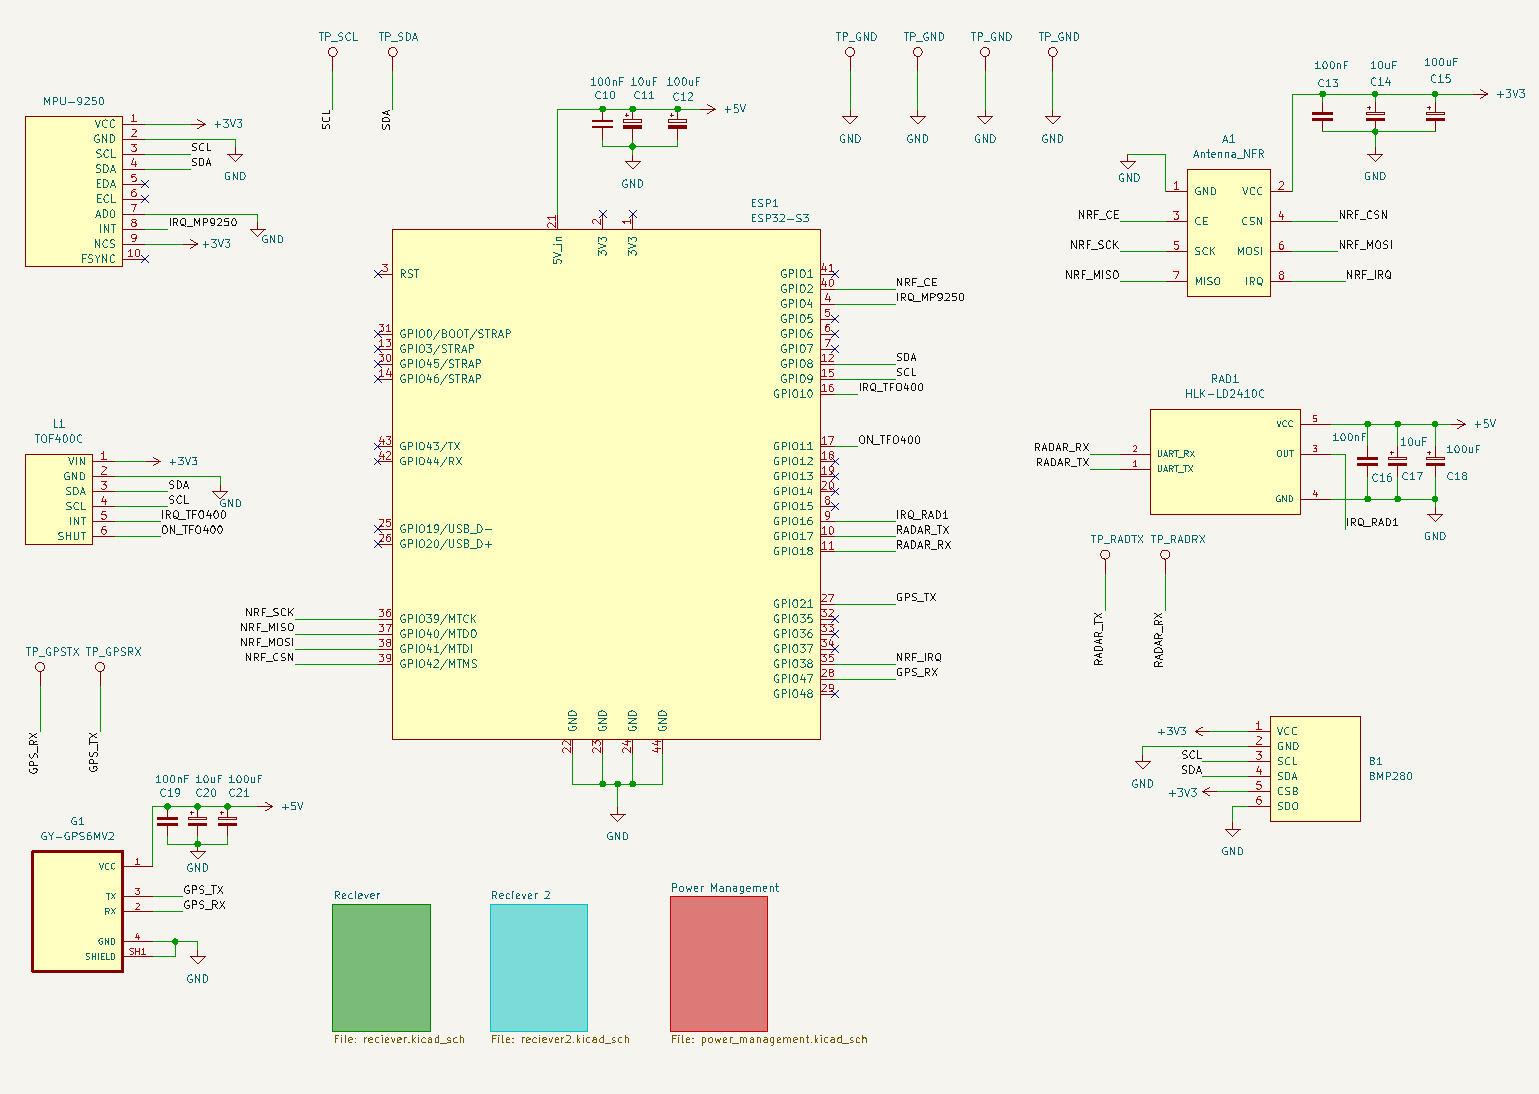
\includegraphics[width=\linewidth]{Figures/transmitter_schematic.pdf}
    \caption{Esquema eléctrico completo del nodo transmisor}
    \label{fig:esquema_kicad_trans}
\end{figure}


\subsection{Nodo receptor}
El nodo receptor se limita al ESP32-C3 Super Mini y al transceptor NRF24L01+, comunicados por SPI, como se muestra en la \cref{fig:esquema_kicad_rec}. Los condensadores de \textit{bulk} situados junto al módulo de radio estabilizan su alimentación durante la recepción.
\begin{figure}[H]
    \centering
    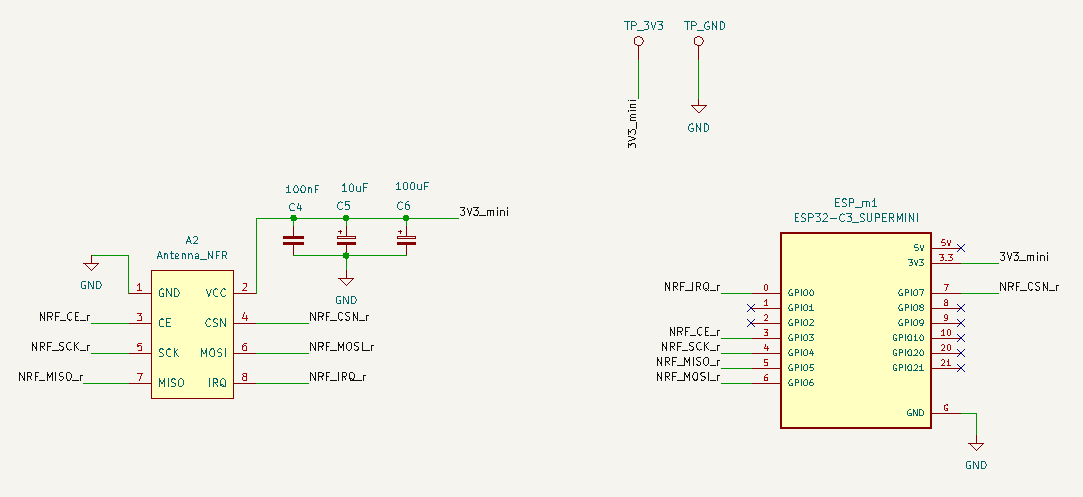
\includegraphics[width=\linewidth]{Figures/reciever_schematic.pdf}
    \caption{Esquema eléctrico completo del nodo receptor}
    \label{fig:esquema_kicad_rec}
\end{figure}

\subsection{Alimentación}
El subsistema de alimentación obtiene el raíl de \SI{5}{\volt} del conector USB-C y genera el de \SI{3.3}{\volt} mediante el LDO NJM12856DL3, como se muestra en la \cref{fig:esquema_kicad_alimentacion}. Los condensadores de desacoplo asociados al regulador son los descritos en la \cref{sec:caps_desacoplo}.
\begin{figure}[H]
    \centering
    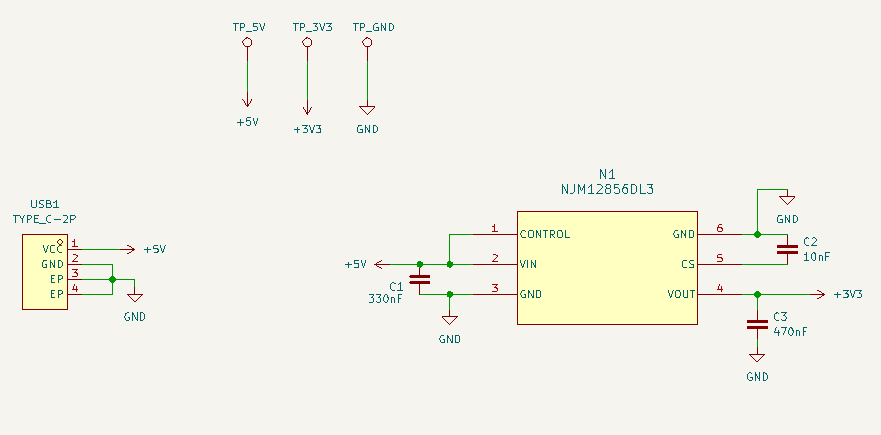
\includegraphics[width=\linewidth]{Figures/power_schematic.pdf}
    \caption{Esquema eléctrico completo del sistema de alimentación}
    \label{fig:esquema_kicad_alimentacion}
\end{figure}


\subsection{Asignación de pines del transmisor}
\label{sec:pines_tx}

La asignación de pines del ESP32-S3 a cada función se resume en la
\cref{tab:pines_tx}. El detalle de todos los pines se puede ver en el esquema eléctrico de la \cref{fig:esquema_kicad_trans}.

\begin{table}[H]
    \centering
    \caption{Asignación de pines del ESP32-S3 (nodo transmisor)}
    \label{tab:pines_tx}
    \footnotesize
    \begin{tabularx}{\linewidth}{l l X}
        \toprule
        \textbf{GPIO} & \textbf{Función} & \textbf{Componente} \\
        \midrule
        GPIO8  & I2C SDA   & MPU-9250, BMP280, VL53L1X \\
        GPIO9  & I2C SCL   & MPU-9250, BMP280, VL53L1X \\
        GPIO21 & UART1 RX  & NEO-6M (TX) \\
        GPIO47 & UART1 TX  & NEO-6M (RX) \\
        GPIO17 & UART2 RX  & HLK-LD2410C (TX) \\
        GPIO18 & UART2 TX  & HLK-LD2410C (RX) \\
        GPIO41 & SPI MOSI  & NRF24L01+ \\
        GPIO40 & SPI MISO  & NRF24L01+ \\
        GPIO39 & SPI SCK   & NRF24L01+ \\
        GPIO42 & SPI CSN   & NRF24L01+ \\
        GPIO2  & GPIO CE   & NRF24L01+ \\
        \bottomrule
    \end{tabularx}
\end{table}

\subsection{Bus I2C: pull-ups y direccionamiento}
\label{sec:bus_i2c}

Los tres sensores I2C no presentan ningún conflicto de direcciones, el MPU-9250 ocupa
\texttt{0x68} con AD0 a GND \cite{ps_mpu9250}, el BMP280 \texttt{0x76}
\cite{ds_bmp280} y el VL53L1X \texttt{0x29} por defecto \cite{ds_vl53l1x}. Por último, el
magnetómetro AK8963 integrado en el MPU-9250 se accede en \texttt{0x0C}
mediante el modo \textit{bypass} del MPU \cite{mpu9250_regmap}.

En cuanto a las resistencias de pull-up, cada módulo \textit{breakout} incluye su propia
pareja de resistencias en SDA y SCL (\SI{10}{\kilo\ohm} hacia
VCC). Al conectar tres módulos en paralelo, la resistencia equivalente cae a
aproximadamente \SI{3.3}{\kilo\ohm}, valor que cae dentro de los límites
recomendados por la especificación I2C de NXP \cite{nxp_i2c} para velocidades
estándar y rápida. Aun así, en el \cref{ch:validacion} se confirma que no hay problemas en el bus.


\subsection{Asignación de pines del receptor}
\label{sec:pines_rx}

El nodo receptor utiliza un ESP32-C3 Super Mini cuyo único componente externo
es el transceptor NRF24L01+ comunicado por SPI (\cref{tab:pines_rx}). El pin
GPIO8 se reserva para el LED \textit{onboard}. La comunicación con el PC se realiza con el conector USB-C nativo
del ESP32-C3 mediante USB-CDC.

\begin{table}[H]
    \centering
    \caption{Asignación de pines del ESP32-C3 Super Mini (nodo receptor)}
    \label{tab:pines_rx}
    \footnotesize
    \begin{tabularx}{\linewidth}{l l X}
        \toprule
        \textbf{GPIO} & \textbf{Función} & \textbf{Notas} \\
        \midrule
        GPIO4 & SPI SCK  & NRF24L01+ \\
        GPIO5 & SPI MISO & NRF24L01+ \\
        GPIO6 & SPI MOSI & NRF24L01+ \\
        GPIO7 & SPI CSN  & NRF24L01+ \\
        GPIO3 & GPIO CE  & NRF24L01+ \\
        GPIO8 & LED      & Onboard \\
        \bottomrule
    \end{tabularx}
\end{table}


\section{Diseño físico de la PCB}
\label{sec:layout}

El diseño físico se ha realizado en KiCad \cite{kicad_pcbnew} sobre una PCB de
dos capas con dimensiones de 180 $\times$ \SI{115}{\milli\meter}. La capa superior
concentra la mayor parte de las señales y rutas de corriente, mientras que la
capa inferior se rellena como plano de masa continuo, con las mínimas trazas posibles, para garantizar la
integridad de señal y reducir las interferencias electromagnéticas. También se ha rellenado la capa superior con masa para mejorar la integridad de la señal y asegurar un retorno correcto de las señales.

\subsection{Restricciones críticas de layout}
\label{sec:layout_restricciones}

Se han aplicado tres restricciones críticas en la disposición de componentes:

\begin{itemize}
    \item \textbf{Keepout de la antena del ESP32-S3.} Se reserva un área sin
    cobre de \SI{15}{\milli\meter} alrededor de la antena PCB del módulo en
    ambas capas, conforme a las recomendaciones del fabricante
    \cite{ds_esp32s3}.

    \item \textbf{Separación entre el radar y la IMU.} El HLK-LD2410C
    transmite a \SI{24}{\giga\hertz} y la IMU es sensible a vibraciones y
    perturbaciones electromagnéticas, por esto se mantienen separados al menos
    \SI{15}{\milli\meter} para minimizar el acoplamiento.

    \item \textbf{Antena del GPS orientada al borde.} El NEO-6M se ubica en
    un borde de la PCB con la antena cerámica hacia el exterior, evitando
    obstáculos metálicos que degradarían la recepción satelital. También se ha dejado un área sin masa alrededor de la antena para minimizar interferencias.
\end{itemize}

\newpage

\subsection{Anchura de pistas y nodo receptor}
\label{sec:layout_pistas}

Se definen dos clases de redes principales con anchuras diferenciadas: \SI{0.25}{\milli
\meter} para señales de baja corriente (I2C, UART, SPI, GPIO) y \SI{1}{
\milli\meter} para las rutas de alimentación. Como se ha mencionado anteriormente, el plano de
masa de la capa inferior se cose a la capa superior mediante un conjunto de
vías distribuidas, reforzando el camino de retorno de las señales.

En cuanto a la PCB del receptor, se ha tomado la decisión de integrar la PCB como una pestaña separable en un borde de la PCB principal, unida mediante pequeñas secciones de PCB. Esto hace que se pueda fabricar ambas PCB en una misma orden de producción, reduciendo el coste global.

En las siguientes figuras se puede ver el diseño de la PCB en el software, y el renderizado 3D final de cómo debería quedar.

\begin{figure}[H]
    \centering
    \includegraphics[width=\linewidth]{Figures/front_pcb_kicad.png}
    \caption{Diseño de la cara superior de la PCB}
    \label{fig:front_pcb_design}
\end{figure}

\begin{figure}[H]
    \centering
    \includegraphics[width=\linewidth]{Figures/back_pcb_kicad.png}
    \caption{Diseño del reverso de la PCB}
    \label{fig:back_pcb_design}
\end{figure}


\begin{figure}[H]
    \centering
    \includegraphics[width=\linewidth]{Figures/iso_pcb.png}
    \caption{Render 3D de la PCB}
    \label{fig:pcb_layout}
\end{figure}

\newpage
\section{Fabricación y ensamblaje}
\label{sec:fabricacion}

La PCB se ha fabricado mediante el servicio JLCPCB, seleccionado por su coste
competitivo (RC01) y su buena calidad. Las especificaciones de fabricación se resumen en la \cref{tab:pcb_fab}.

\begin{table}[H]
    \centering
    \caption{Especificaciones de fabricación de la PCB}
    \label{tab:pcb_fab}
    \footnotesize
    \begin{tabularx}{0.75\linewidth}{l X}
        \toprule
        \textbf{Parámetro} & \textbf{Valor} \\
        \midrule
        % TODO: confirma los valores reales que pediste en JLCPCB
        Fabricante           & JLCPCB \\
        Número de capas      & 2 \\
        Dimensiones          & 180 $\times$ \SI{115}{\milli\meter} \\
        Espesor              & \SI{1.6}{\milli\meter} \\
        Grosor de cobre      & 1~oz (\SI{35}{\micro\meter}) \\
        Acabado superficial  & HASL \\
        \bottomrule
    \end{tabularx}
\end{table}


\begin{figure}[H]
    \centering
    \begin{subfigure}[b]{0.45\linewidth}
        \centering
        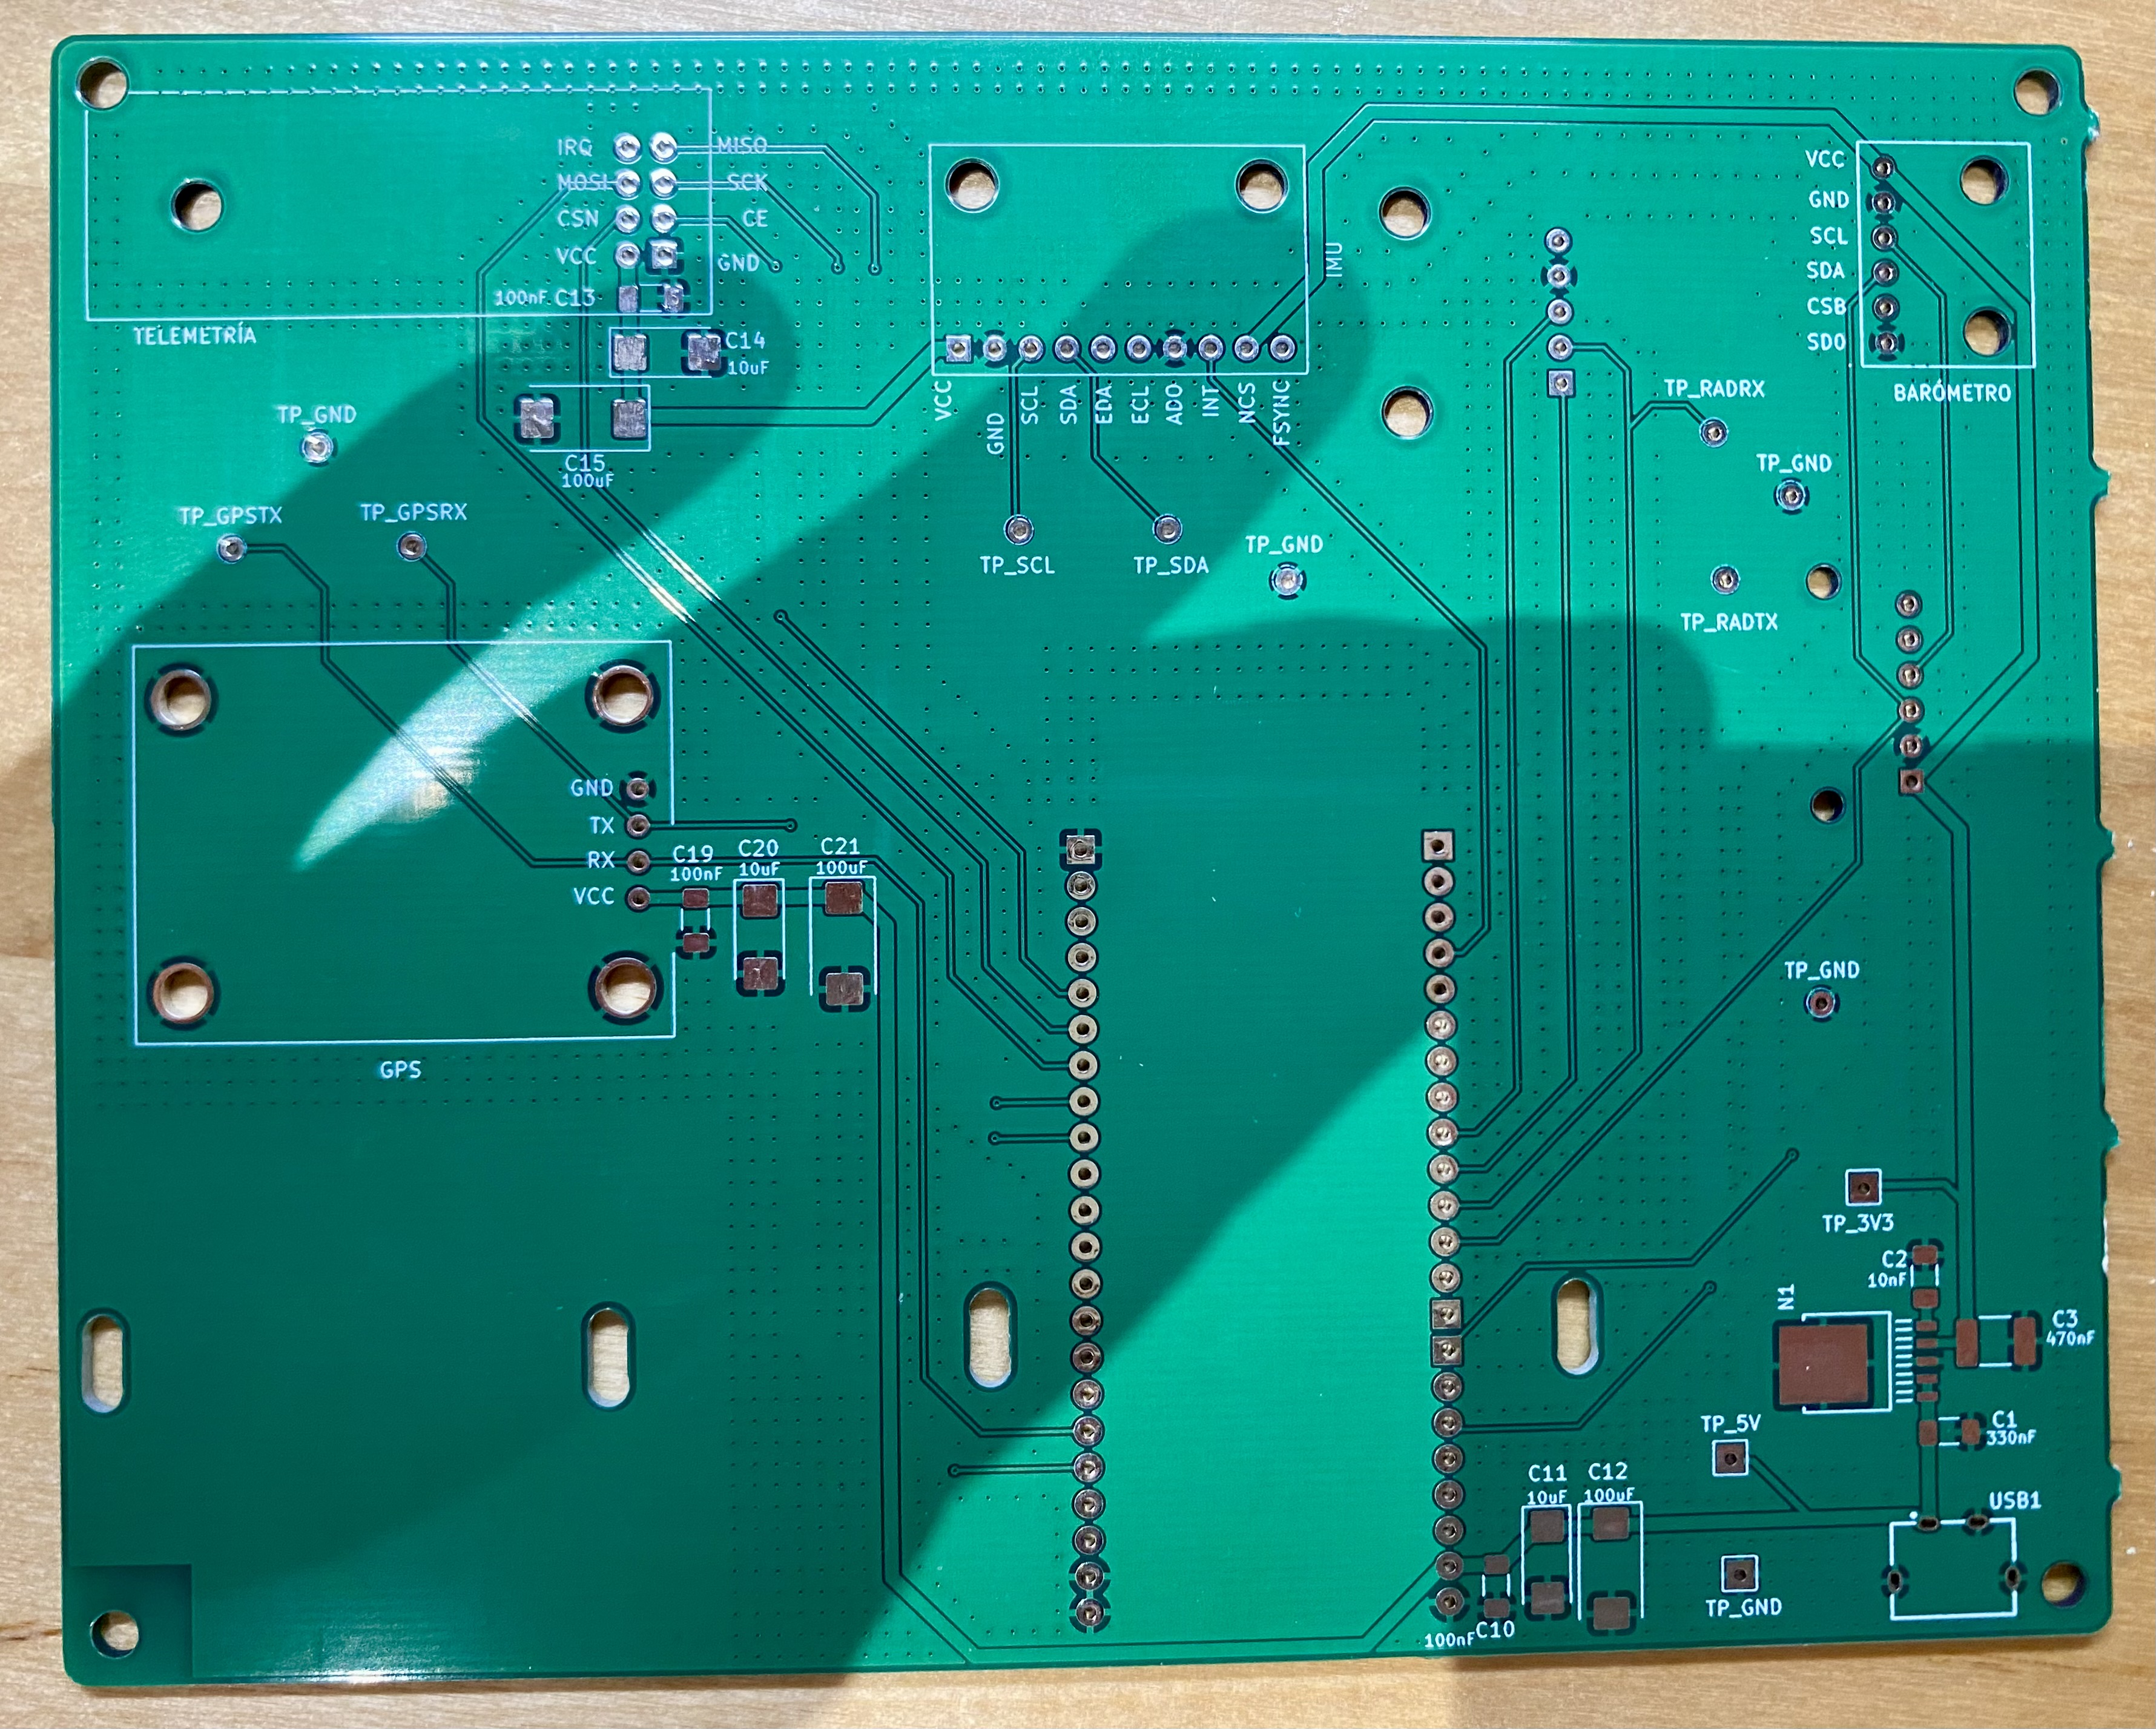
\includegraphics[width=\linewidth]{Figures/front_pcb.jpeg}
        \caption{Cara superior de la PCB}
        \label{fig:cara_pcb_fabricada}
    \end{subfigure}
    \hfill
    \begin{subfigure}[b]{0.45\linewidth}
        \centering
        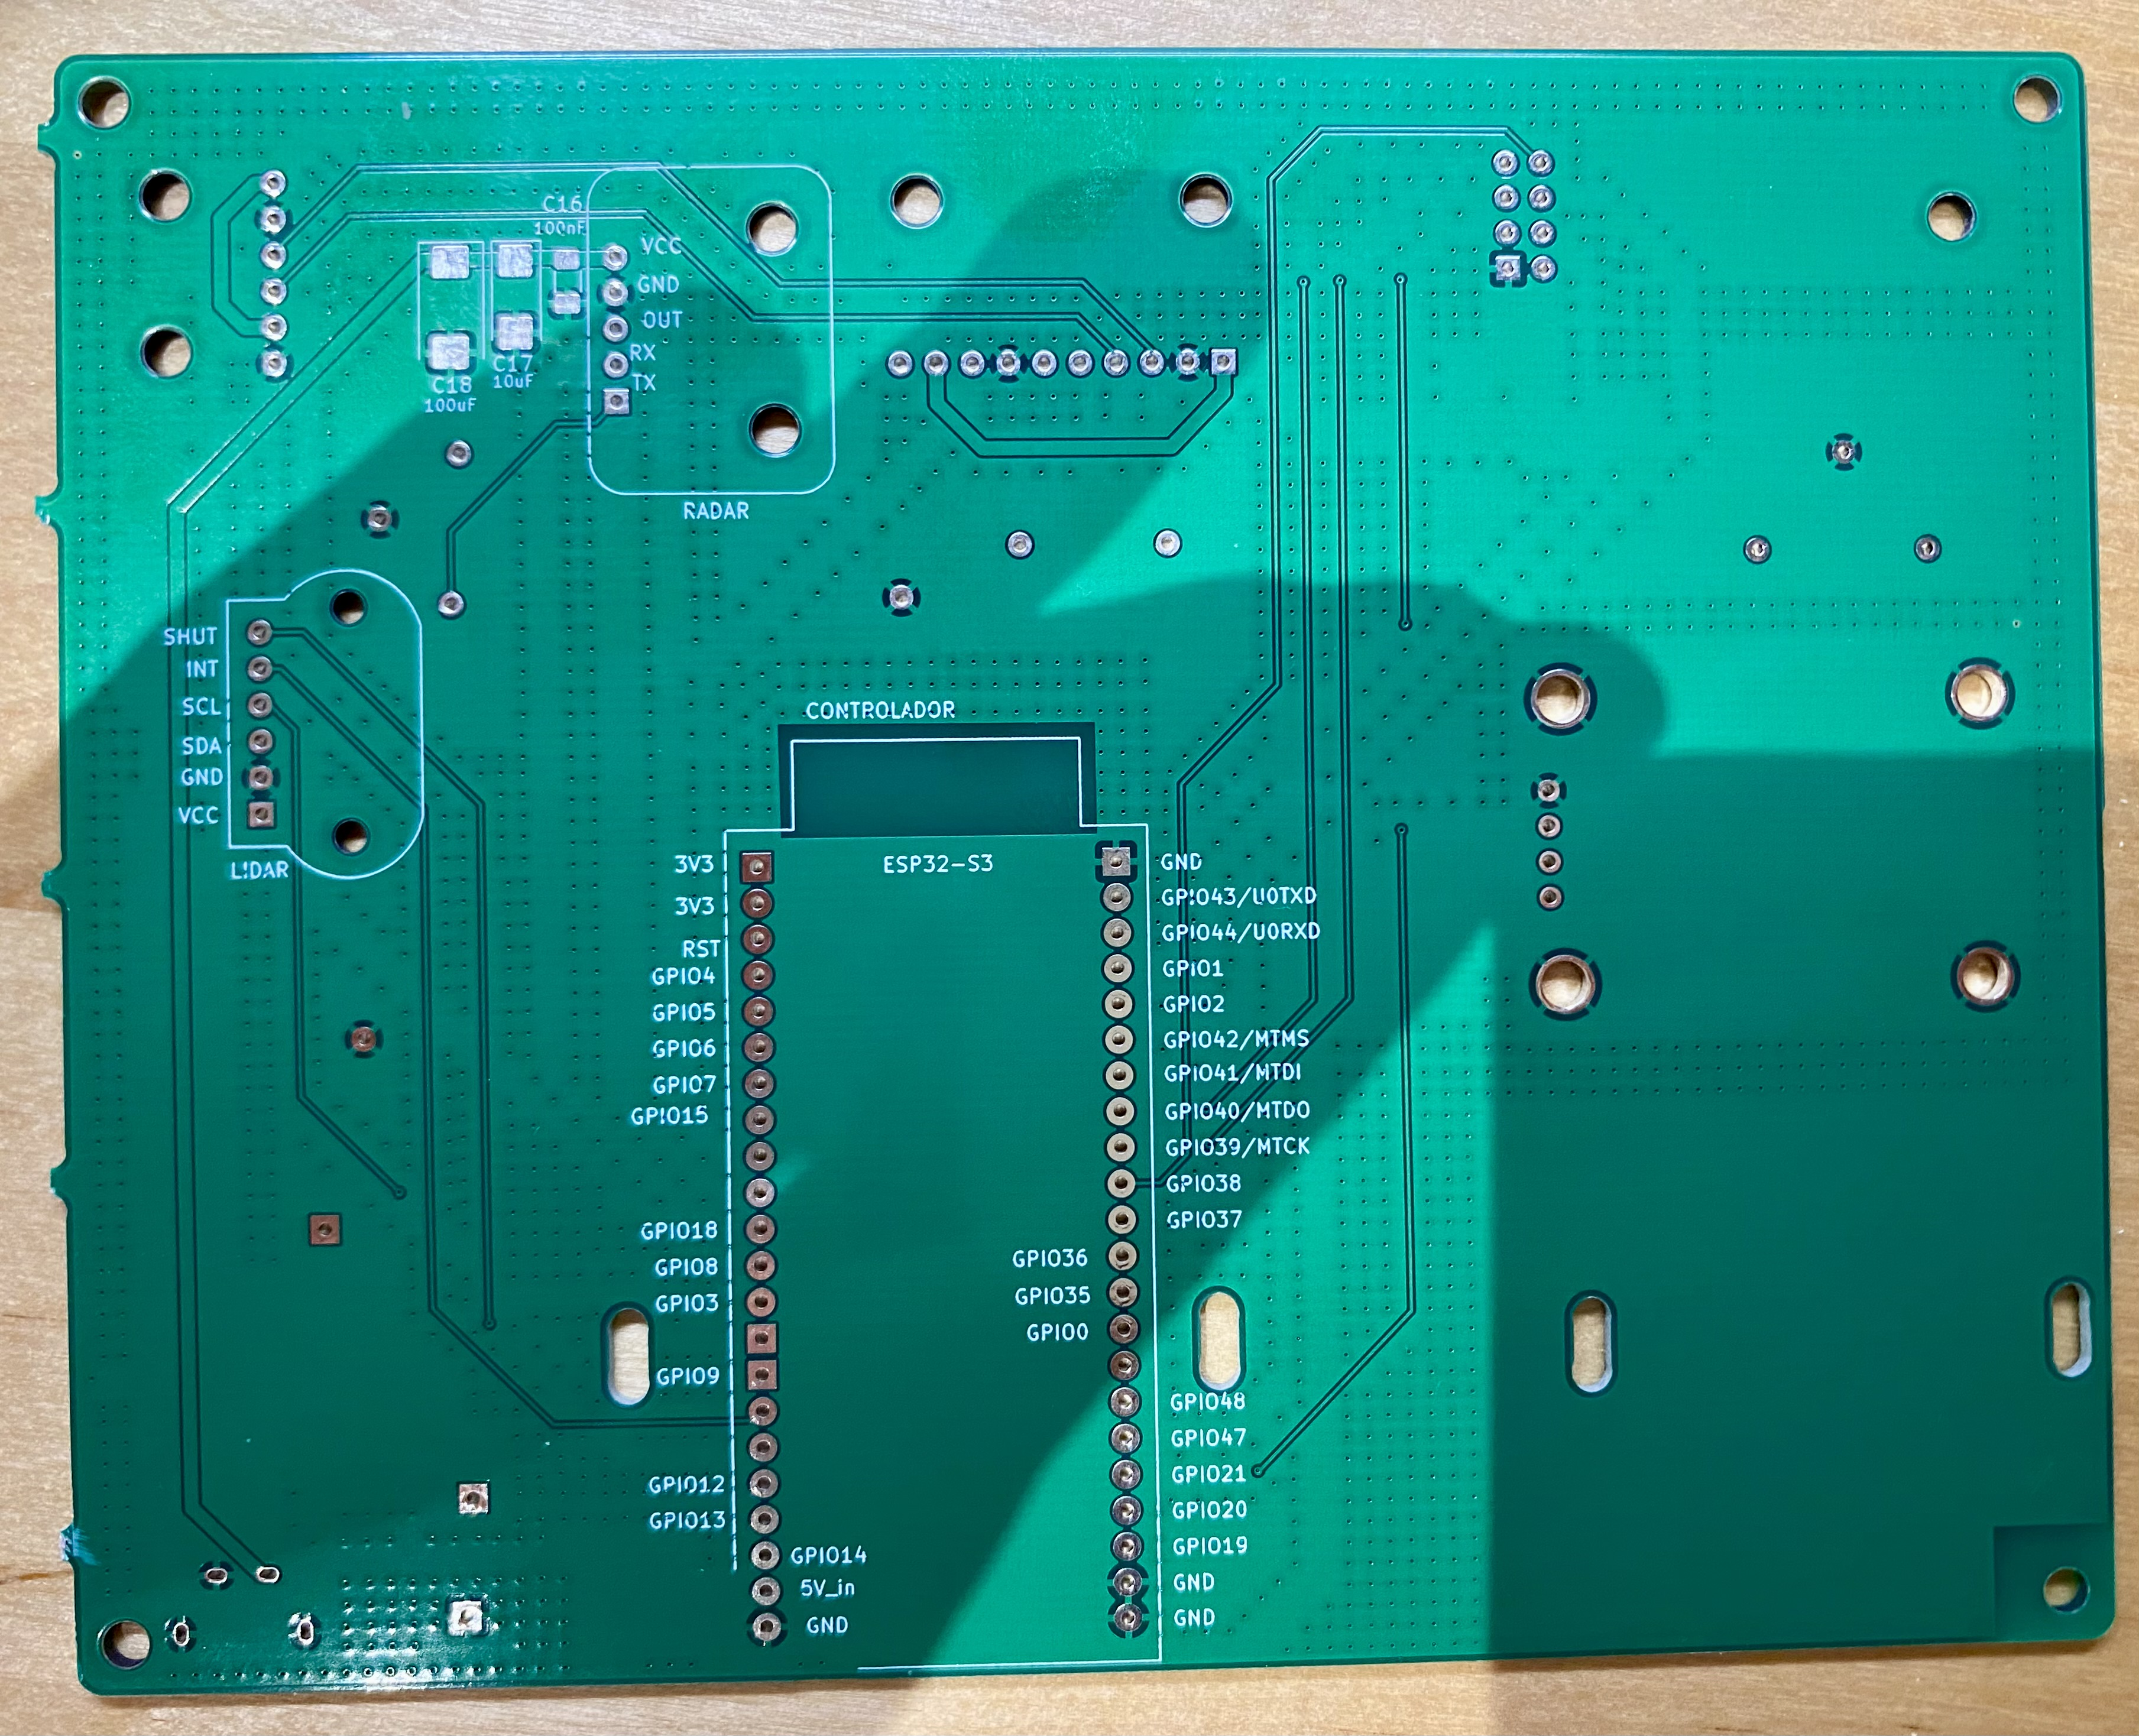
\includegraphics[width=\linewidth]{Figures/back_pcb.jpeg}
        \caption{Reverso de la PCB}
        \label{fig:reverso_pcb_fabricada}
    \end{subfigure}
    \caption{PCB del nodo transmisor antes de incorporar ningún componente}
    \label{fig:transmitter_pcb}
\end{figure}
\begin{figure}[H]
    \centering
    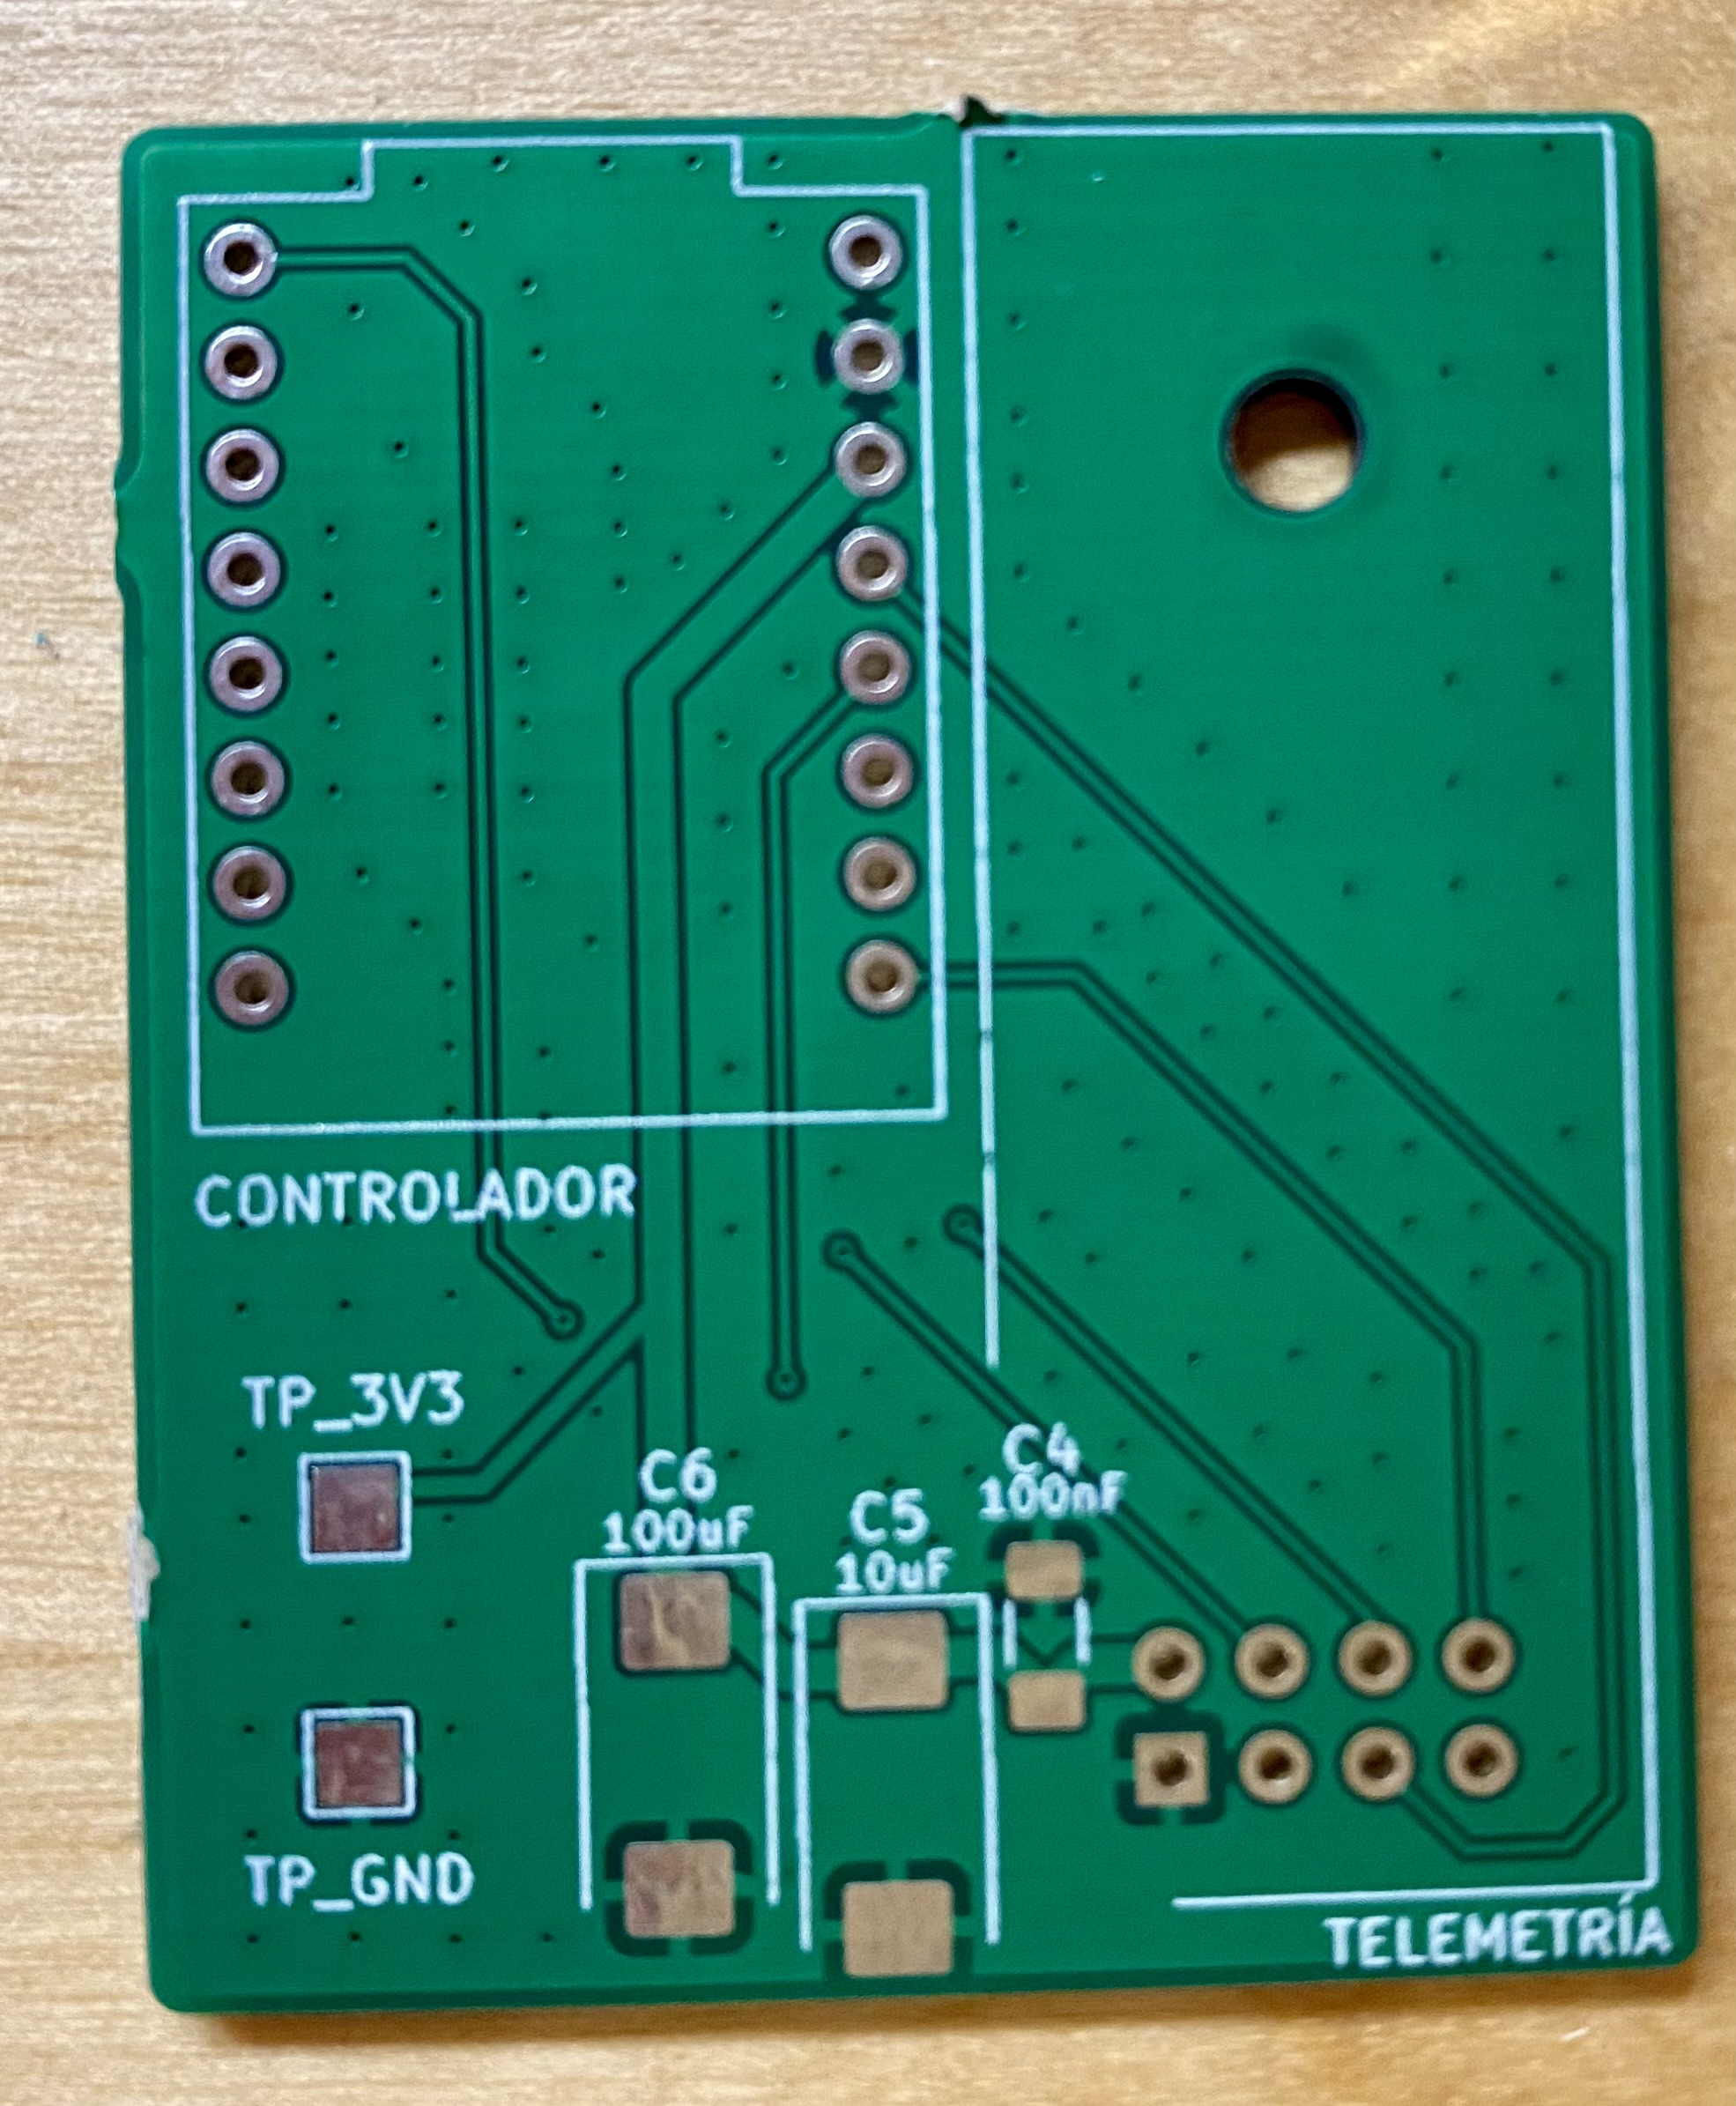
\includegraphics[width=0.35\textwidth]{Figures/reciever_pcb.jpeg}
    \caption{PCB del nodo receptor antes de incorporar ningún componente}
    \label{fig:reciever_pcb}
\end{figure}

Una vez obtenida la PCB, primero se verifica que no hay ningún defecto a simple vista antes de proceder al ensamblaje, y luego se separa el receptor de la PCB principal. El ensamblaje se realiza de forma manual mediante soldador convencional. Los componentes pasivos en formato SMD se sueldan primero, seguidos
del LDO, el conector USB-C y, por último los zócalos hembra para los módulos
\textit{breakout}. La elección de zócalos en lugar de soldadura directa de los componentes a la PCB permite sustituir los módulos durante el desarrollo y reutilizarlos en futuras iteraciones, además de facilitar la sustitución en caso de fallo de algún componente.

\begin{figure}[H]
    \centering
    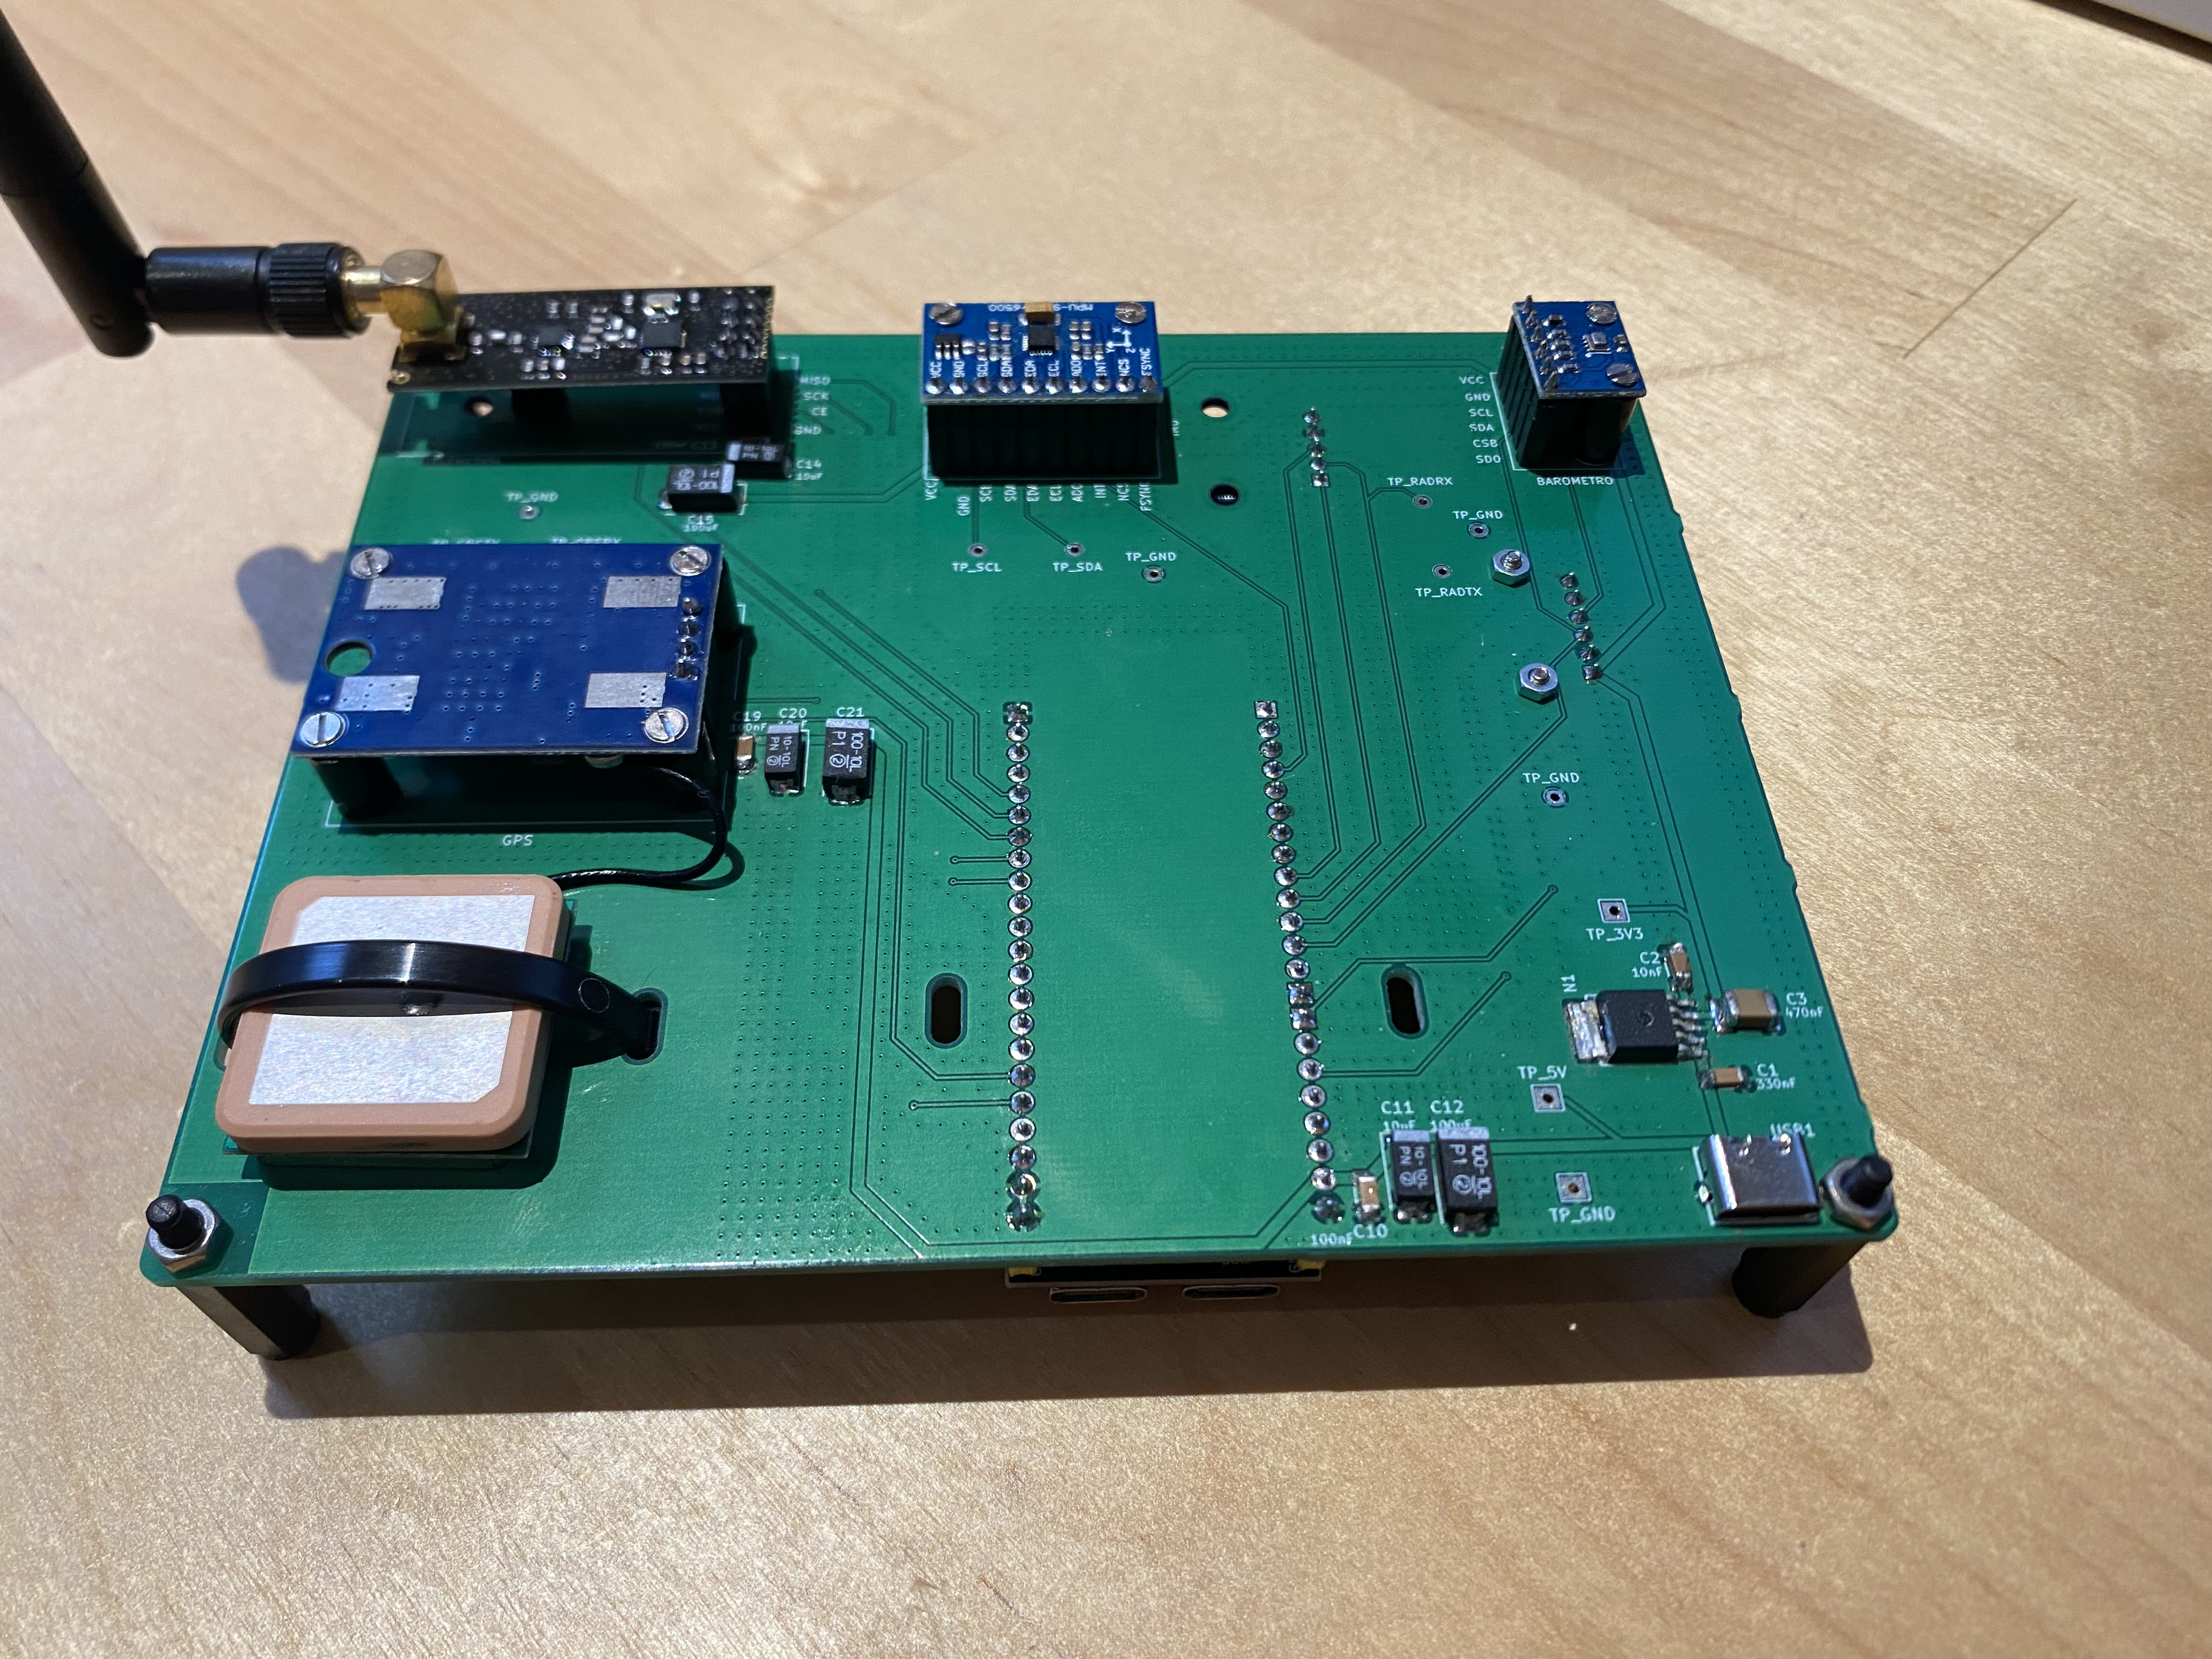
\includegraphics[width=0.70\linewidth]{Figures/real_pcb.jpeg}
    \caption{PCB del nodo transmisor totalmente ensamblada con todos los
    módulos incorporados}
    \label{fig:pcb_ensamblado}
\end{figure}

\begin{figure}[H]
    \centering
    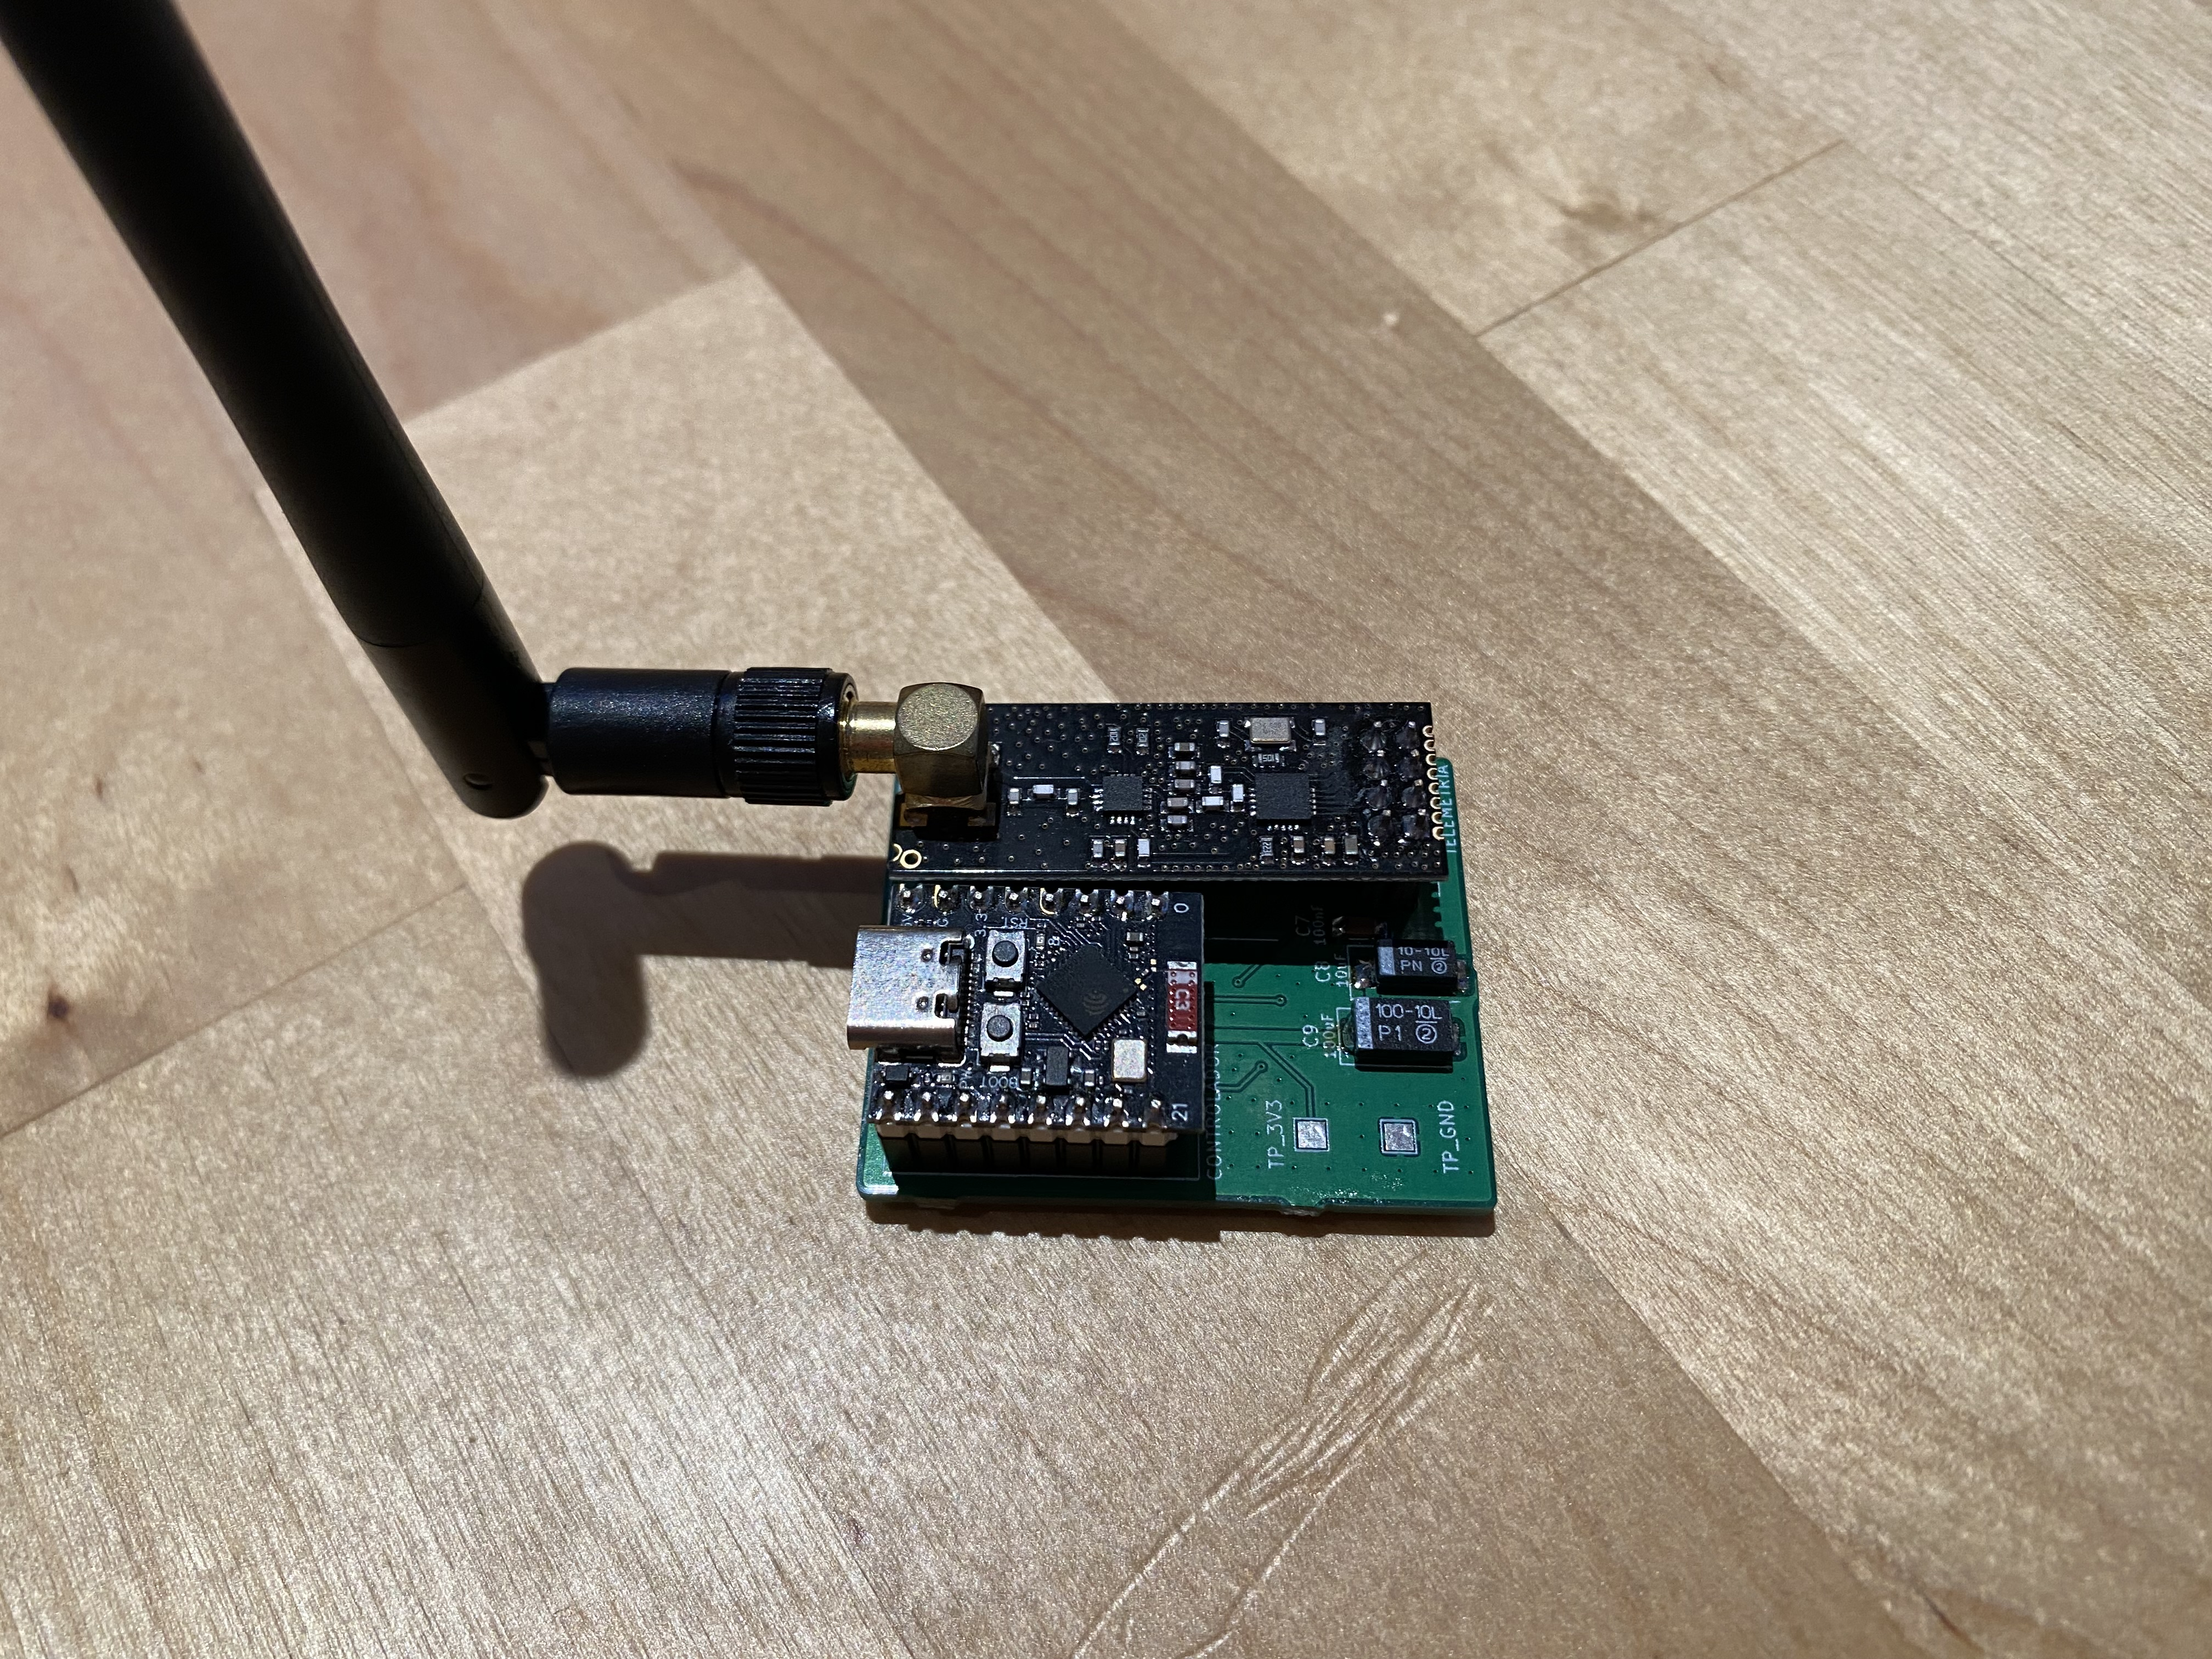
\includegraphics[width=0.70\linewidth]{Figures/real_reciever_pcb.jpeg}
    \caption{PCB del nodo receptor totalmente ensamblada con todos los
    módulos incorporados}
    \label{fig:pcb__receptor_ensamblado}
\end{figure}

El coste total del sistema, incluyendo fabricación de la PCB, componentes
pasivos y módulos \textit{breakout}, se desglosa en la \cref{tab:bom_resumen}
de la \cref{sec:sel_resumen}.

\section{Verificación del hardware}
\label{sec:verificacion}

Antes de cargar el firmware se realizaron dos pruebas de \textit{bring-up}
sobre la PCB. Primero, una verificación de continuidad con el multímetro y
la placa sin alimentar, contrastando las \textit{nets} contra el
\textit{netlist} del esquemático y descartando cortocircuitos entre los
planos de alimentación y masa, para asegurar que no había cortocircuitos producidos en el proceso de soldadura. No se detectaron circuitos abiertos ni cortocircuitos. Después, ya con la
placa alimentada por USB-C y sin carga, se midieron los \textit{rails} de
\SI{5}{\volt} y \SI{3.3}{\volt}, que quedaron dentro de las tolerancias del
regulador NJM12856DL3 \cite{ds_njm12856}. Al final se confirmó el funcionamiento correcto de todos los módulos del sistema.
\cleardoublepage

% Capítulo 6: Diseño del Firmware
%!TEX root = ../main.tex

\chapter{Diseño de firmware}
\label{ch:firmware}

El \cref{ch:hardware} ha definido la plataforma física sobre la que se ejecuta
el firmware. En este capítulo se detalla el software que adquiere las
medidas de los sensores, las fusiona para obtener las magnitudes de vuelo y las
transmite codificadas en ARINC 429 hasta el nodo receptor. Se describe primero
el firmware del nodo transmisor, después la capa lógica de telemetría
compartida por ambos nodos y, por último, el firmware del nodo receptor. La
visualización en el PC se trata en el \cref{ch:software}.


\section{Entorno de desarrollo y organización del código}
\label{sec:fw_entorno}

Ambos nodos se programan sobre el framework de Arduino para ESP32
\cite{ds_esp32s3, ds_esp32c3}, lo que cumple la restricción de herramientas de
código abierto (RC02) y mantiene un único entorno compartido por el transmisor
y el receptor.

El firmware del transmisor se organiza de forma modular. Cada sistema se compila de forma individual en su propia unidad de compilación, mientras que dos cabeceras compilan los elementos comunes entre todos los nodos. \texttt{SensorData.h} define las estructuras de datos
que comparten todos los módulos y \texttt{Config.h} agrupa en un único lugar todas las constantes: pines, escalas de los
sensores, ganancias del filtro, declinación magnética y constantes de
calibración. Esta separación permite sustituir o corregir un driver sin afectar
al resto y deja un único archivo donde reconfigurar la plataforma. Las
bibliotecas empleadas se resumen en la \cref{tab:fw_libs}.

\begin{table}[H]
    \centering
    \caption{Bibliotecas empleadas en el firmware del transmisor}
    \label{tab:fw_libs}
    \footnotesize
    \begin{tabularx}{\linewidth}{l l X}
        \toprule
        \textbf{Subsistema} & \textbf{Biblioteca} & \textbf{Función} \\
        \midrule
        IMU + magnetómetro & acceso a registros propio & Lectura del MPU-9250 y el AK8963 (\cite{kriswiner_mpu9250}). \\
        Barómetro          & Adafruit\_BMP280 \cite{lib_bmp280} & Configuración y lectura del BMP280. \\
        GPS                & TinyGPSPlus \cite{lib_tinygps} & Parseo de tramas NMEA del NEO-6M. \\
        Radar              & MyLD2410 \cite{lib_myld2410} & Configuración y lectura del HLK-LD2410C. \\
        ToF                & VL53L1X (Pololu) \cite{lib_vl53l1x} & Lectura del VL53L1X. \\
        Radio              & RF24 \cite{lib_rf24} & Control del nRF24L01+. \\
        Bus I2C            & Wire (Arduino core) & Bus compartido de los sensores I2C. \\
        \bottomrule
    \end{tabularx}
\end{table}

La \cref{fig:fw-arquitectura-tx-vertical} resume la organización del sistema. El flujo
nace en los sensores físicos, pasa por cada uno de sus drivers y por las
estructuras de \texttt{SensorData.h}, se procesa en la fusión y converge en la
capa de telemetría que multiplexa los parámetros y los transmite.

\begin{figure}[H]
  \centering
  \resizebox{0.7\textwidth}{!}{%
  \begin{tikzpicture}[
      font=\small,
      >={Stealth[length=2.2mm]},
      hw/.style  ={draw, rounded corners=2pt, fill=black!6,  minimum height=8mm, minimum width=26mm, align=center},
      drv/.style ={draw, fill=blue!10,   minimum height=8mm, minimum width=24mm, align=center},
      dat/.style ={draw, fill=green!12,  minimum height=7mm, minimum width=22mm, align=center},
      proc/.style={draw, fill=orange!18, minimum height=8mm, minimum width=26mm, align=center},
      tel/.style ={draw, fill=red!12,    minimum height=12mm, minimum width=154mm, align=center},
      rf/.style  ={draw, fill=violet!12, minimum height=8mm, minimum width=40mm, align=center},
      ctl/.style ={draw, dashed, fill=yellow!18, align=center, rounded corners=2pt, text width=145mm, inner sep=3mm},
      df/.style  ={->, thick},
      cf/.style  ={->, dashed, gray, thick}
    ]

    % --- Orquestador loop() (Capa superior) ---
    \node[ctl, fill=cyan!12] (loop) at (0, 3.5)
        {FlightInstruments.ino :: loop() -- planificador cooperativo\\
         IMU+fusión 100 Hz, barómetro 10 Hz, telemetría 20 Hz; GPS/radar/ToF cada iteración (no bloqueante)};

    % --- Config.h (Ahora debajo del loop y sobre los sensores) ---
    \node[ctl] (cfg) at (0, 1.7)
        {Config.h -- parametros: pines, escalas, ganancias Kp/Ki, declinación, calibración hard/soft iron};

    % --- Sensores (Capa Hardware, y=0) ---
    \node[hw] (s_imu)   at (-6.4, 0) {MPU-9250\\+ AK8963};
    \node[hw] (s_baro)  at (-3.2, 0) {BMP280};
    \node[hw] (s_tof)   at (0, 0)    {VL53L1X};
    \node[hw] (s_gps)   at (3.2, 0)  {NEO-6M};
    \node[hw] (s_radar) at (6.4, 0)  {HLK-LD2410C};

    % --- Drivers (y=-2) ---
    \node[drv] (d_imu)   at (-6.4, -2) {IMU.ino};
    \node[drv] (d_baro)  at (-3.2, -2) {Barometer.ino};
    \node[drv] (d_tof)   at (0, -2)    {ToF.ino};
    \node[drv] (d_gps)   at (3.2, -2)  {GPS.ino};
    \node[drv] (d_radar) at (6.4, -2)  {Radar.ino};

    % --- Estructuras (SensorData.h, y=-4) ---
    \node[dat] (st_imu)   at (-6.4, -4) {RawIMU};
    \node[dat] (st_baro)  at (-3.2, -4) {BaroData};
    \node[dat] (st_tof)   at (0, -4)    {ToFData};
    \node[dat] (st_gps)   at (3.2, -4)  {GPSData};
    \node[dat] (st_radar) at (6.4, -4)  {RadarData};

    % --- Procesamiento (y=-6 y -7.5 en la columna izquierda) ---
    \node[proc] (fusion) at (-6.4, -6.0) {SensorFusion.ino\\(Mahony MARG)};
    \node[dat]  (flight) at (-6.4, -7.5) {FlightData};

    % --- Telemetria (Embudo horizontal, y=-9.5) ---
    \node[tel] (tele) at (0, -9.5)
        {Telemetry.ino (planificador EDF por etiqueta) \\ {}[\textit{lib}] ARINC429};

    % --- Salida radio (y=-11.5) ---
    \node[rf] (nrf) at (0, -11.5) {NRF24L01+PA+LNA};

    % ================= RUTADO DE FLECHAS =================

    % --- Flujo Hardware -> Driver ---
    \draw[df] (s_imu)   -- node[right,font=\scriptsize]{I2C}   (d_imu);
    \draw[df] (s_baro)  -- node[right,font=\scriptsize]{I2C}   (d_baro);
    \draw[df] (s_tof)   -- node[right,font=\scriptsize]{I2C}   (d_tof);
    \draw[df] (s_gps)   -- node[right,font=\scriptsize]{UART1} (d_gps);
    \draw[df] (s_radar) -- node[right,font=\scriptsize]{UART2} (d_radar);

    % --- Flujo Driver -> Estructura ---
    \draw[df] (d_imu)   -- (st_imu);
    \draw[df] (d_baro)  -- (st_baro);
    \draw[df] (d_tof)   -- (st_tof);
    \draw[df] (d_gps)   -- (st_gps);
    \draw[df] (d_radar) -- (st_radar);

    % --- Flujo Fusión (Columna IMU) ---
    \draw[df] (st_imu) -- (fusion);
    \draw[df] (fusion) -- (flight);

    % --- Flujo hacia Telemetría ---
    \draw[df] (flight)   -- (flight |- tele.north);
    \draw[df] (st_baro)  -- (st_baro |- tele.north);
    \draw[df] (st_tof)   -- (st_tof |- tele.north);
    \draw[df] (st_gps)   -- (st_gps |- tele.north);
    \draw[df] (st_radar) -- (st_radar |- tele.north);

    % --- Telemetría -> Radio ---
    \draw[df] (tele) -- (nrf);
    \draw[df] (nrf.east) -- ++(2,0) 
        node[right,align=left,font=\scriptsize]{enlace 2.4 GHz\\-> nodo receptor};

    % --- Dependencia cruzada (Gating Doppler) ---
    \draw[cf] (st_gps.east) to[out=0,in=180] 
        node[right,font=\scriptsize,align=left]{$v_{GPS}$\\(Doppler)} (d_radar.west);

    % --- Enlaces de control (loop y config) ---
    \draw[cf] (loop.south) -- (cfg.north);
    \draw[cf] (cfg.south)  -- (0, 0.8); % Línea indicativa hacia la capa de hardware/drivers

  \end{tikzpicture}%
  }
  \caption{Arquitectura modular top-down del firmware. Se ilustra el flujo completo de los datos, desde el hardware hasta la transmisión final.}
  \label{fig:fw-arquitectura-tx-vertical}
\end{figure}

\section{Bucle principal y planificación cooperativa}
\label{sec:fw_loop}

El nodo transmisor no utiliza un sistema operativo en tiempo real, sino una planificación cooperativa más sencilla. En cada loop del bucle principal (loop()), el programa revisa unos temporizadores y ejecuta solo las tareas cuyo periodo se ha cumplido. De este modo, cada subsistema funciona a su propia frecuencia sin interrumpir a los demás.

Las tareas y sus frecuencias se resumen en la \cref{tab:fw_rates}. La
adquisición de datos de la IMU y la fusión se ejecutan a \SI{100}{\hertz}, el barómetro a
\SI{10}{\hertz} y la telemetría a \SI{20}{\hertz}, coherente con el RP03 y con
el periodo de \SI{50}{\milli\second} del enlace. Los buffers UART del GPS y del
radar se vacían en cada iteración, ya que si se descuidan aunque sea un ciclo, la
UART se satura y se pierden tramas. El ToF y el GPS se leen de forma oportunista, en cada iteración se consulta el sensor y la estructura se actualiza únicamente cuando hay datos válidos disponibles, conservando el último valor conocido en caso contrario.

\begin{table}[H]
    \centering
    \caption{Tareas del bucle principal del transmisor}
    \label{tab:fw_rates}
    \begin{tabularx}{\linewidth}{X l l}
        \toprule
        \textbf{Tarea} & \textbf{Frecuencia} & \textbf{Mecanismo} \\
        \midrule
        Adquisición inercial + fusión & \SI{100}{\hertz} & Temporizada (\texttt{micros}) \\
        Lectura del barómetro         & \SI{10}{\hertz}  & Temporizada (\texttt{millis}) \\
        Envío de telemetría           & \SI{20}{\hertz}  & Temporizada (\texttt{millis}) \\
        Alimentación de UART (GPS, radar) & Cada iteración & Sondeo continuo \\
        Lectura de ToF y GPS          & Oportunista       & Sondeo por disponibilidad \\
        \bottomrule
    \end{tabularx}
\end{table}



En cuanto a la inicialización de los sensores se aplica una jerarquía de criticidad. La IMU es el único
sensor cuyo fallo detiene el arranque, ya que es el único sensor esencial, sin él no hay horizonte artificial. El resto de sensores se tratan de forma distinta, si alguno no responde, el sistema continúa y su parámetro se transmite con el SSM en estado
NO\_DATA (\cref{sec:fw_word}), que el receptor descarta.


\section{Adquisición inercial}
\label{sec:fw_imu}

La IMU MPU-9250 integra acelerómetro y giroscopio y, conectado internamente, el
magnetómetro AK8963. El driver (\texttt{IMU.ino}) accede directamente a los
registros de los 3 sensores a través del bus I2C compartido a \SI{400}{\kilo\hertz},
siguiendo las hojas de datos \cite{ps_mpu9250, ds_ak8963}.

Tras comprobar el registro de identidad, el acelerómetro se configura a
$\pm 4\,g$ y el giroscopio a $\pm 500\,^{\circ}/\mathrm{s}$, con un filtro
digital interno a unos \SI{42}{\hertz}. El AK8963 no es accesible directamente,
por lo que se habilita el modo \textit{bypass} del MPU-9250 para hacerlo visible en el
bus. A continuación se lee su matriz de sensibilidad de fábrica (ASA), la cual corrige la ganancia de cada eje, y se configura en modo
continuo de 16 bits a \SI{100}{\hertz}.

Un detalle relevante de implementación es la diferencia de \textit{endianness}
entre ambos integrados: el MPU-9250 entrega los datos en formato big-endian y el
AK8963 en little-endian, por lo que la composición de los bytes difiere para
cada uno. La aceleración, la temperatura y el giro se leen en una única ráfaga
de 14 bytes. La lectura del magnetómetro exige leer también su registro de
estado para que prepare la siguiente muestra.

El pipeline completo del magnetómetro consiste de 3 etapas desde la lectura de los datos: la conversión a microteslas
con la sensibilidad de fábrica (ASA), la resta del offset de hierro duro y el
reescalado por el factor de hierro blando. El valor final queda de la forma siguiente:
\begin{equation}
    m_i^{\text{cal}} = s_i\,\bigl(k\,\mathrm{ASA}_i\,\tilde{m}_i - b_i\bigr),
    \qquad i \in \{x,y,z\}
\end{equation}
donde $\tilde{m}_i$ es la lectura base, $k$ la sensibilidad nominal, y
$b_i$ y $s_i$ provienen de la calibración realizada, descrita en la
\cref{sec:fw_calibracion}, cuyas constantes quedan  fijadas en \texttt{Config.h}.


\section{Calibración}
\label{sec:fw_calibracion}

\subsection{Bias del giroscopio}
\label{sec:fw_cal_gyro}

El bias del giroscopio se estima en cada arranque (\texttt{Calibration.ino}). Se
promedian \num{500} muestras con el sensor en reposo y se calcula su varianza;
si la varianza máxima de los tres ejes queda por debajo de un umbral, la media
se acepta como bias. Si se detecta movimiento durante la captura (varianza
alta), se descarta el valor y se recurre a un valor por defecto obtenido previamente.
Teóricamente, el término integral podría converger al valor correcto sin la calibración inicial, pero de esta forma la convergencia es mucho más rápida.

\subsection{Calibración del magnetómetro (hierro duro y blando)}
\label{sec:fw_cal_mag}

La calibración de hierro duro y blando del magnetómetro se realiza una sola vez
con el sistema completo en funcionamiento (radio transmitiendo y resto de
sensores activos) y lejos de estructuras ferromagnéticas. Calibrar así, con todos los sensores activos es
necesario porque el offset de hierro duro no recoge únicamente los materiales
magnetizados, sino también el campo generado por las corrientes continuas de la
propia placa. La rutina se compila condicionalmente en el firmware principal, activada por la macro
\texttt{CALIBRATE\_MAG}, así se hace la calibración y después esa parte del código no se compila en condición de uso normal. Los datos se recogen con el sensor girando lentamente en todas las orientaciones durante \SI{30}{\second}, se registran los valores mínimo y máximo
de cada eje. El offset de hierro duro centra el elipsoide medida en el origen
y el factor de hierro blando lo reescala hacia una esfera:
\begin{equation}
    b_i = \tfrac{1}{2}\bigl(m_i^{\max}+m_i^{\min}\bigr), \qquad
    s_i = \frac{\bar{r}}{r_i}, \quad
    r_i = \tfrac{1}{2}\bigl(m_i^{\max}-m_i^{\min}\bigr)
\end{equation}
con $\bar{r}$ el radio medio de los tres ejes. 
Los seis valores obtenidos (1 por cada eje, para blando y duro) se fijan como constantes en \texttt{Config.h}.

Por otro lado, la declinación magnética (diferencia entre el norte magnético medido y el norte
geográfico) se añade como constante en la fusión. El rumbo resultante es ligeramente sensible al entorno magnético. En condiciones de campo limpio se mantiene estable, mientras que en interiores las distorsiones del campo magnético local
lo degradan de forma notable. Esta degradación en interiores se cuantifica en el
\cref{ch:validacion}.


\section{Fusión de actitud: filtro de Mahony}
\label{sec:fw_fusion}

En la fusión de la actitud y el rumbo se emplea el filtro complementario no lineal de Mahony sobre el grupo $SO(3)$ \cite{mahony2008}, el cual va alimentado por los 9 ejes de la IMU (acelerómetro, giroscopio y magnetómetro). La decisión de por qué se elige este filtro ya ha sido explicada en \cref{sec:ea_fusion}. También la decisión de implementar la fusión en firmware, en lugar de delegarla a un sensor con fusión integrada, se justificó en la \cref{sec:sel_imu} por su valor docente.

El núcleo del filtro corrige la medida del giroscopio basándose en un error de
orientación construido a partir de las direcciones de la gravedad y del campo
magnético. El error es la suma de los productos vectoriales entre cada vector
medido (normalizado) y su dirección esperada según el cuaternión actual se expresa como:

\begin{equation}
    \mathbf{e} = \mathbf{a}\times\hat{\mathbf{v}}_g + \mathbf{m}\times\hat{\mathbf{v}}_m
\end{equation}
Para que el rumbo no afecte a la corrección de inclinación, el vector magnético de referencia se
proyecta eliminando su componente transversal. El controlador PI corrige la velocidad angular
y se integra el cuaternión, que se renormaliza en cada paso:
\begin{equation}
    \hat{\omega} = \omega_g + K_p\,\mathbf{e} + K_i\!\int \mathbf{e}\,dt,
    \qquad
    \dot{\mathbf{q}} = \frac{1}{2}\,\mathbf{q}\otimes(0,\hat{\omega})
\end{equation}
La \cref{fig:mahony_block} resume esta estructura.

\begin{figure}[H]
    \centering
    \resizebox{\textwidth}{!}{%
    \begin{tikzpicture}[
        font=\small, >=Stealth,
        blk/.style={draw, rounded corners=2pt, align=center, minimum height=9mm, inner sep=3pt, fill=black!5},
        io/.style ={draw, align=center, minimum height=9mm, inner sep=3pt, fill=blue!8},
        sum/.style={draw, circle, minimum size=6mm, inner sep=0pt}]

        % fila superior
        \node[io]  (gyro) {Giroscopio\\$\omega_g$};
        \node[sum, right=14mm of gyro] (sum) {\large$+$};
        \node[blk, right=12mm of sum]  (int)  {Integración del\\cuaternión};
        \node[blk, right=10mm of int]  (norm) {Normalización};
        \node[draw, circle, inner sep=1pt, right=10mm of norm, fill=green!12] (q) {$\mathbf{q}$};
        \node[blk, right=10mm of q]    (euler){Ángulos de\\Euler (P,R,H)};

        % fila inferior
        \node[io]  (am)  at ($(gyro)+(0,-22mm)$) {Acelerómetro $\mathbf{a}$\\Magnetómetro $\mathbf{m}$};
        \node[blk] (err) at ($(int)+(0,-22mm)$)  {Error de orientación\\$\mathbf{e}=\mathbf{a}\times\hat{\mathbf{v}}_g+\mathbf{m}\times\hat{\mathbf{v}}_m$};
        \node[blk] (pi)  at ($(norm)+(0,-22mm)$) {Controlador PI\\$K_p\,\mathbf{e}+K_i\!\int\!\mathbf{e}\,dt$};

        \draw[->] (gyro) -- (sum);
        \draw[->] (sum)  -- (int);
        \draw[->] (int)  -- (norm);
        \draw[->] (norm) -- (q);
        \draw[->] (q)    -- (euler);
        \draw[->] (am)   -- (err);
        \draw[->] (err)  -- (pi);

        % corrección PI hacia el sumador
        \draw[->] (pi) -- ([yshift=6mm]pi.north) -| (sum)
            node[pos=0.25, above, font=\scriptsize] {corrección};

        % realimentación del cuaternión hacia el error
        \draw[->, dashed] (q.south) -- ($(q.south)+(0,-31mm)$) -| (err.south)
            node[pos=0.25, below, font=\scriptsize] {actitud estimada $\mathbf{q}$};
    \end{tikzpicture}%
    }
    \caption{Estructura del filtro complementario de Mahony. La velocidad
             angular del giroscopio se corrige con un término PI cuyo error
             procede de la gravedad y el campo magnético medidos frente a sus
             direcciones esperadas según el cuaternión, que se realimenta.}
    \label{fig:mahony_block}
\end{figure}

El cuaternión se convierte a ángulos de Euler y de ahí al convenio aeronáutico
NED. En este punto se aplican pequeños offsets de montaje en cabeceo y alabeo, la declinación magnética y el offset entre el adelante de la IMU y el de la PCB, valores que se recogen en (\cref{tab:mahony_params}). Inicialmente el magnetómetro se reorienta al sistema de ejes del acelerómetro y giroscopio, ya que están rotados entre sí. Para que el filtro arranque ya cerca de la orientación real,
el cuaternión se inicializa mediante un alineamiento analítico inicial (acelerómetro y magnetómetro) a partir de una sola muestra, en lugar de partir del cuaternión identidad.

\begin{table}[H]
    \centering
    \caption{Parámetros del filtro de Mahony y correcciones de actitud}
    \label{tab:mahony_params}
    \begin{tabularx}{\linewidth}{X l l}
        \toprule
        \textbf{Parámetro} & \textbf{Símbolo} & \textbf{Valor} \\
        \midrule
        Ganancia proporcional  & $K_p$ & \num{3.0} \\
        Ganancia integral      & $K_i$ & \num{1.0} \\
        Declinación magnética  & --    & $1.95^{\circ}$ \\
        Offset de montaje (cabeceo) & -- & $0.6^{\circ}$ \\
        Offset de montaje (alabeo)  & -- & $0.2^{\circ}$ \\
        Offset de rumbo (IMU--PCB)  & -- & $-5.0^{\circ}$ \\
        Tasa de actualización  & --    & \SI{100}{\hertz} \\
        \bottomrule
    \end{tabularx}
\end{table}


\section{Adquisición barométrica}
\label{sec:fw_baro}

El barómetro BMP280 (\texttt{Barometer.ino}, biblioteca de Adafruit
\cite{lib_bmp280}) se configura con sobremuestreo de presión $\times 16$, de
temperatura $\times 2$, filtro IIR $\times 16$ y modo normal con un tiempo de
reposo de \SI{62.5}{\milli\second}. Esta combinación de tiempo de conversión y
reposo da una tasa de salida próxima a los \SI{10}{\hertz} de lectura.

La altitud sobre el nivel del mar se obtiene de la presión mediante la fórmula
de la atmósfera estándar \cite{icao_isa}, con la presión de referencia a nivel
del mar utilizada $p_0 = \SI{1013.25}{\hecto\pascal}$:
\begin{equation}
    h = 44330\left[1 - \left(\frac{p}{p_0}\right)^{0{,}1903}\right]
\end{equation}
La velocidad vertical se calcula por diferencias finitas de la altitud y
se suaviza con un filtro exponencial (EMA). El filtro IIR interno del sensor reduce el ruido de presión, pero la
discriminación del LSB hace que la derivada directa avance a saltos, por esto se aplica el EMA.

\begin{equation}
    v_s[k] = (1-\alpha)\,v_s[k-1] + \alpha\,\frac{h[k]-h[k-1]}{\Delta t},
    \qquad \alpha = 0{,}2
\end{equation}



\section{Posicionamiento GNSS}
\label{sec:fw_gps}

El receptor NEO-6M (\texttt{GPS.ino}) se lee mediante la biblioteca TinyGPSPlus
sobre UART1. Sus bytes se alimentan en cada iteración del bucle para no perder
tramas NMEA. El driver distingue dos estados: \textit{ok}, que indica que la
UART recibe datos aunque no haya satélites suficientes para determinar posición, y \textit{fix}, que
indica posición válida. Los campos derivados (altitud, velocidad, rumbo de
tierra y satélites) solo se refrescan cuando el dato correspondiente es válido,
conservando el último valor conocido en caso contrario.

El NEO-6M es un receptor exclusivamente GPS, sin GLONASS ni Galileo, lo que limita la precisión de los valores a \SI{2.5}{\meter} CEP. La tasa de actualización que ofrece es suficiente para la frecuencia a la que el
planificador retransmite los parámetros GPS (\cref{sec:scheduler}).


\section{Sensores de proximidad}
\label{sec:fw_proximidad}

La medida de distancia al suelo se aborda con dos sensores de tecnología
distinta, acorde con (RF06). El telémetro láser de tiempo de vuelo VL53L1X es el sensor
principal y el radar FMCW HLK-LD2410C el secundario. La
razón de esta jerarquía es la fiabilidad observada. El ToF entrega una distancia
métrica estable, mientras que la clasificación del radar es ambigua y sensible
al \textit{clutter}.

\paragraph{Tiempo de vuelo.}
El VL53L1X (\texttt{ToF.ino}, biblioteca de Pololu \cite{lib_vl53l1x}) se
configura en modo de largo alcance (hasta \SI{4}{\meter}) con un presupuesto
de tiempo de \SI{50}{\milli\second} por medida y lectura continua a
\SI{20}{\hertz}. La lectura es no bloqueante, solo actualiza la estructura cuando
hay una muestra lista. Por debajo de una zona muerta de \SI{40}{\milli\meter} la
medida se marca como no válida.

\paragraph{Radar.}
El HLK-LD2410C (\texttt{Radar.ino}, biblioteca MyLD2410) es un radar de
\SI{24}{\giga\hertz} que reparte el alcance en puertas de distancia. Se
configura en alta resolución (\SI{20}{\centi\meter} por puerta, 9 puertas,
alcance \SI{1.8}{\meter}). Los
umbrales por puerta se ajustan a una orientación hacia el suelo: umbrales altos
en las puertas cercanas, para rechazar el \textit{clutter} del propio chasis y
la vibración, y bajos en las lejanas, para no perder el suelo a mayor distancia.
Sobre la distancia de la puerta dominante (la de mayor energía) se aplica un
suavizado EMA y un valor mínimo que descarta ecos residuales de baja energía.

Además, el sensor dispone de clasificación Doppler, para distinguir entre objetivos móviles y estáticos. El problema es que en este uso, puede ser que esté en movimiento la placa y no el objetivo. Por esto, esta clasificación se habilita únicamente
cuando la velocidad GPS está por debajo de un umbral de reposo. Ambas distancias
se transmiten en la telemetría (el ToF como radioaltímetro, el radar como
distancia de radar), pero el PFD utiliza el ToF como única fuente 
(\cref{ch:software}).


\section{Implementación de la telemetría ARINC 429}
\label{sec:arinc_hw}

Como se introdujo en la \cref{sec:arinc_arq}, la telemetría se codifica en la
capa lógica del estándar ARINC 429 \cite{arinc429}. La capa física diferencial
del estándar no se implementa, ya que el transporte es a través de radiofrecuencia. Esta
sección detalla el formato de palabra, las etiquetas, la codificación BNR, la
paridad y el SSM (RN04), así como la estructura del paquete y el planificador que
reparte los parámetros sobre el enlace. La biblioteca \texttt{ARINC429},
desarrollada para el proyecto, implementa la construcción y decodificación de
palabras y es compartida por ambos nodos.

\subsection{Formato de palabra}
\label{sec:fw_word}

Cada palabra ARINC 429 ocupa 32 bits repartidos en cinco campos
(\cref{fig:arinc_word}): la etiqueta (\textit{label}, 8 bits en octal)
identifica el parámetro, el SDI (2 bits) identifica origen o destino, el campo
de datos (19 bits) transporta los valores, el SSM (2 bits) indica el estado del
dato, y el bit de paridad cierra la palabra.

\begin{figure}[H]
    \centering
    \setlength{\tabcolsep}{3pt}\renewcommand{\arraystretch}{1.2}
    \begin{tabularx}{\linewidth}{|c|c|>{\centering\arraybackslash}X|c|c|}
        \hline
        \cellcolor{orange!18}P & SSM & \cellcolor{blue!8}Datos (BNR / discreta) & SDI & \cellcolor{background_light}Label (octal) \\
        \scriptsize 32 & \scriptsize 31--30 & \scriptsize bits 29--11 (19 bits) & \scriptsize 10--9 & \scriptsize bits 8--1 \\
        \hline
    \end{tabularx}
    \caption{Formato de la palabra ARINC 429 de 32 bits.}
    \label{fig:arinc_word}
\end{figure}

Los parámetros numéricos se codifican en formato binario BNR. El valor se escala
por una resolución por bit (LSB) y se almacena como entero con signo de 19 bits
en complemento a dos, saturando si excede el rango:
\begin{equation}
    D = \mathrm{round}\!\left(\frac{x}{\text{LSB}}\right),
    \qquad D \in \left[-2^{18},\, 2^{18}-1\right]
\end{equation}
La \cref{tab:arinc_labels} recoge las etiquetas empleadas con su codificación y
resolución. Las etiquetas de actitud, rumbo, altitudes, velocidad vertical y
posición son estándar, mientras que la distancia de radar y la palabra de estado usan
etiquetas libres no asignadas por la norma.

\begin{table}[H]
    \centering
    \caption{Etiquetas ARINC 429 empleadas (etiqueta en octal)}
    \label{tab:arinc_labels}
    \footnotesize
    \begin{tabularx}{\linewidth}{X c c l}
        \toprule
        \textbf{Parámetro} & \textbf{Etiqueta} & \textbf{Cod.} & \textbf{LSB} \\
        \midrule
        Cabeceo (pitch)        & 0324  & BNR & $180/2^{18}\ {}^{\circ}$ \\
        Alabeo (roll)          & 0325  & BNR & $180/2^{18}\ {}^{\circ}$ \\
        Rumbo magnético        & 0320  & BNR & $180/2^{18}\ {}^{\circ}$ \\
        Altitud barométrica    & 0204  & BNR & \num{0.5} ft \\
        Velocidad vertical     & 0365  & BNR & \num{0.125} ft/min \\
        Altitud GPS            & 0076  & BNR & \num{0.5} ft \\
        Radioaltímetro (ToF)   & 0164  & BNR & \num{0.0625} ft \\
        Distancia de radar     & 0166$^{*}$ & BNR & \SI{0.01}{\meter} \\
        Latitud$^{\dagger}$    & 0310  & BNR & $1/2^{18}\ {}^{\circ}$ \\
        Longitud$^{\dagger}$   & 0311  & BNR & $1/2^{18}\ {}^{\circ}$ \\
        Estado (status)        & 0270$^{*}$ & discreta & -- \\
        \bottomrule
    \end{tabularx}

    \vspace{2pt}
    {\footnotesize $^{*}$ etiqueta libre, no asignada por la norma.\\
    $^{\dagger}$ codificada como desplazamiento respecto a una referencia local
    ($41^{\circ}$,\,$1^{\circ}$) para alcanzar mejor resolución .}
\end{table}

El SSM toma cuatro valores: operación normal, sin datos, prueba funcional y
fallo. El firmware transmite \textsc{normal} cuando el dato es válido y
\textsc{no\_data} cuando el sensor correspondiente está fuera de servicio. El
receptor descarta cualquier palabra que no sea \textsc{normal}. Por último, el
bit 32 implementa paridad impar, se fija de modo que el número total de unos de
la palabra sea impar, lo que permite al receptor detectar palabras corruptas.

La latitud y la longitud emplean etiquetas estándar, pero con una resolución por
bit más fina que la nominal. Con una única palabra BNR de 19 bits y rango global
(\(\pm 180^{\circ}\)), la posición quedaría cuantizada a una rejilla de unos
\SI{76}{\meter}, muy por encima del error del receptor. Por ello se codifica el
desplazamiento respecto a una referencia local fija, lo que reduce el rango a
\(\pm 1^{\circ}\) y mejora la resolución hasta unos \SI{0.42}{\meter}. El receptor
reconstruye la coordenada absoluta sumando de nuevo dicha referencia.

\subsection{Estructura del paquete de telemetría}
\label{sec:estructura_paquete}

El payload del nRF24L01+ es de \SI{32}{\byte}, valor que coincide exactamente con 8
palabras ARINC 429 de 32 bits. Esta coincidencia permite evitar fragmentar el paquete
(\cref{sec:enlace}). Las tres primeras palabras transportan siempre la actitud y
el rumbo, los parámetros más críticos, en cada paquete a \SI{20}{\hertz}, las
cinco restantes se multiplexan entre el resto de parámetros según el
planificador de la \cref{sec:scheduler}.

\begin{figure}[H]
    \centering
    \begin{tikzpicture}[node distance=0mm, font=\footnotesize]

        \def\slotW{16mm}
        \def\slotH{12mm}

        % Slots fijos
        \node[block, fill=background_light, minimum width=\slotW, minimum height=\slotH]
            (s0) {Slot 0\\\footnotesize Pitch};
        \node[block, fill=background_light, minimum width=\slotW, minimum height=\slotH, right=of s0]
            (s1) {Slot 1\\\footnotesize Roll};
        \node[block, fill=background_light, minimum width=\slotW, minimum height=\slotH, right=of s1]
            (s2) {Slot 2\\\footnotesize Heading};

        % Slots multiplexados
        \node[block, minimum width=\slotW, minimum height=\slotH, right=of s2] (s3) {Slot 3};
        \node[block, minimum width=\slotW, minimum height=\slotH, right=of s3] (s4) {Slot 4};
        \node[block, minimum width=\slotW, minimum height=\slotH, right=of s4] (s5) {Slot 5};
        \node[block, minimum width=\slotW, minimum height=\slotH, right=of s5] (s6) {Slot 6};
        \node[block, minimum width=\slotW, minimum height=\slotH, right=of s6] (s7) {Slot 7};

        % Llaves superiores (¡Direccion corregida de izquierda a derecha!)
        \draw [decorate, decoration={brace, amplitude=4pt, raise=2pt}]
            (s0.north west) -- (s2.north east)
            node[midway, above=6pt, font=\footnotesize\itshape] {Fijos (20\,Hz)};
        \draw [decorate, decoration={brace, amplitude=4pt, raise=2pt}]
            (s3.north west) -- (s7.north east)
            node[midway, above=6pt, font=\footnotesize\itshape] {Multiplexados (EDF)};

        % Etiqueta inferior centrada bajo todo el paquete
        \node[below=4mm of s3.south east, font=\footnotesize]
            {Paquete completo: 8 palabras x 32 bits = 32 bytes, enviado a 20\,Hz};

    \end{tikzpicture}
    \caption{Estructura del paquete de telemetría sobre el payload de
             \SI{32}{\byte} del nRF24L01+.}
    \label{fig:estructura_paquete}
\end{figure}

\subsection{Planificador de tasas}
\label{sec:scheduler}

Cada parámetro multiplexado tiene un periodo nominal (\cref{tab:scheduler_assignment}).
En cada paquete, los cinco slots disponibles se asignan con una política del
tipo \textit{earliest deadline first} (EDF): para cada parámetro se calcula su
retraso respecto a su periodo nominal y se eligen, de mayor a menor retraso. Si en un slot no hay ningún parámetro pendiente, se rellena
con una palabra vacía (etiqueta 0, SSM \textsc{no\_data}) que el receptor
ignora. La palabra de estado incorpora un número de secuencia que permite al
receptor estimar la salud del enlace a partir de las palabras de estado perdidas
(a \SI{5}{\hertz}).

La viabilidad del reparto se comprueba sumando la demanda de los parámetros
multiplexados: cuatro a \SI{10}{\hertz} y cuatro a \SI{5}{\hertz} requieren
$4\times10 + 4\times5 = \num{60}$ palabras por segundo, frente a las
$5\times20 = \num{100}$ ranuras multiplexadas disponibles. El margen resultante
absorbe los retrasos puntuales sin que ningún parámetro supere su periodo. Se
emplea EDF en lugar de un turno fijo (\textit{round-robin}) porque prioriza
automáticamente el parámetro más atrasado, lo que acota el retraso máximo de cada
magnitud.

\begin{table}[H]
    \centering
    \caption{Asignación de parámetros del planificador}
    \label{tab:scheduler_assignment}
    \begin{tabularx}{\linewidth}{l X l}
        \toprule
        \textbf{Parámetro} & \textbf{Magnitud} & \textbf{Tasa} \\
        \midrule
        Pitch & Cabeceo & \SI{20}{\hertz} (slot fijo) \\
        Roll & Alabeo & \SI{20}{\hertz} (slot fijo) \\
        Heading & Rumbo magnético & \SI{20}{\hertz} (slot fijo) \\
        \midrule
        Pres.~altitude & Altitud barométrica & \SI{10}{\hertz} \\
        Vertical speed & Velocidad vertical & \SI{10}{\hertz} \\
        Radar distance & Distancia radar & \SI{10}{\hertz} \\
        Radio altitude & Distancia ToF (radioaltímetro) & \SI{10}{\hertz} \\
        \midrule
        GPS altitude & Altitud GPS & \SI{5}{\hertz} \\
        Latitude & Latitud & \SI{5}{\hertz} \\
        Longitude & Longitud & \SI{5}{\hertz} \\
        Status & Estado y validez del sistema & \SI{5}{\hertz} \\
        \bottomrule
    \end{tabularx}
\end{table}


La configuración  del transceptor adoptada se resume en la \cref{tab:nrf24_config}.
La tasa de \num{250}~kbps se elige por su buen compromiso entre
sensibilidad y velocidad: un paquete completo con reconocimiento ocupa
aproximadamente \SI{2}{\milli\second}, dentro del periodo de
\SI{50}{\milli\second} fijado por la tasa de \SI{20}{\hertz} de la
arquitectura. La potencia se ajusta al máximo, optimizando para uso
en interior con obstáculos.

\begin{table}[H]
    \centering
    \caption{Configuración del transceptor nRF24L01+ adoptada}
    \label{tab:nrf24_config}
    \begin{tabularx}{\linewidth}{l X}
        \toprule
        \textbf{Parámetro} & \textbf{Valor} \\
        \midrule
        Frecuencia portadora        & Banda ISM \SI{2.4}{\giga\hertz} \\
        Tasa de datos               & \num{250}~kbps \\
        Tamaño de payload           & \SI{32}{\byte} (fijo) \\
        CRC                         & 2 bytes (habilitado) \\
        Reconocimiento automático   & Habilitado (Enhanced ShockBurst) \\
        Reintentos automáticos      & Hasta 15 (Enhanced ShockBurst) \\
        Nivel de potencia de salida & Máximo del módulo PA/LNA \\
        \bottomrule
    \end{tabularx}
\end{table}


\section{Nodo receptor}
\label{sec:fw_receptor}

El nodo receptor (ESP32-C3 Super Mini, \texttt{FlightInstruments\_Receiver.ino})
recibe los paquetes por el enlace y los entrega al PC. Su transceptor nRF24L01+
se configura con el mismo canal y tasa que el transmisor.

\paragraph{Decodificación.}
Cada paquete se procesa palabra a palabra: se comprueba la paridad, se descartan
las palabras vacías o corruptas y, según la etiqueta, se actualiza el campo
correspondiente de una caché de estado. Esta caché funciona como
\textit{hold-last-good}, cada parámetro conserva su último valor válido y solo
se refresca cuando llega una palabra con SSM \textsc{normal}. Como excepción, el
radioaltímetro (ToF) y la distancia de radar se ponen a cero cuando su palabra
llega sin datos, de modo que el indicador de proximidad no se queda congelado en
un valor antiguo.

\paragraph{Detección de pérdidas.}
A partir del número de secuencia, que viaja en la palabra de estado a
\SI{5}{\hertz} (contador de 6 bits, módulo 64), el receptor detecta huecos entre
palabras de estado: un salto distinto del esperado se contabiliza como palabra de
estado perdida, salvo que sea muy grande, en cuyo caso se asume un reinicio del
transmisor. Este recuento es un indicador de salud del enlace a \SI{5}{\hertz}, no
una medida exacta de pérdida de paquetes. Cada
segundo se emite un resumen de estadísticas del enlace y, tras \SI{3}{\second}
sin recibir nada, un aviso de enlace caído.

\paragraph{Salida al PC.}
El estado decodificado se envía por serial a \SI{20}{\hertz} como una frase de
texto delimitada por comas (\texttt{\$TEL}), con las conversiones de unidades que
espera el PFD. La sentencia se emite por dos vías en paralelo
(\cref{fig:rx_dataflow}): el puerto serie USB, que es la vía empleada por el PFD
de Processing (\cref{ch:software}), y un \textit{broadcast} UDP sobre un punto de
acceso WiFi propio del receptor, pensado para visualización en un dispositivo Android.

\begin{figure}[H]
    \centering
    \resizebox{\textwidth}{!}{%
    \begin{tikzpicture}[
        font=\small, >=Stealth,
        blk/.style={draw, rounded corners=2pt, align=center, minimum height=9mm, inner sep=3pt, fill=black!5},
        io/.style ={draw, align=center, minimum height=9mm, inner sep=3pt, fill=blue!8}]
        \node[io]  (nrf) {NRF24L01+\\(recepción)};
        \node[blk, right=10mm of nrf] (dec) {\texttt{processWord()}\\paridad + SSM};
        \node[blk, right=10mm of dec] (st)  {\texttt{DecodedState}\\\textit{hold-last-good}};
        \node[blk, right=10mm of st]  (tel) {Serialización\\sentencia \texttt{\$TEL}};
        \node[io, above right=5mm and 12mm of tel] (pc)  {Serial USB\\$\rightarrow$ PC (PFD)};
        \node[io, below right=5mm and 12mm of tel] (udp) {UDP broadcast\\$\rightarrow$ cliente móvil};
        \draw[->] (nrf) -- (dec);
        \draw[->] (dec) -- (st);
        \draw[->] (st)  -- (tel);
        \draw[->] (tel) -- (pc);
        \draw[->] (tel) -- (udp);
    \end{tikzpicture}%
    }
    \caption{Cadena de procesamiento del nodo receptor: decodificación palabra a
             palabra, caché de último valor válido y doble salida hacia el PC
             (serie USB) y hacia un cliente móvil (UDP).}
    \label{fig:rx_dataflow}
\end{figure}

\paragraph{Una limitación documentada.}
Hay un aspecto de la telemetría que conviene señalar. Dos de los indicadores de estado que
llegan al PFD (IMU y radio) se fuerzan a \textit{correcto} de forma incondicional
en cuanto llega cualquier paquete, por lo que no reflejan la salud real de esos
subsistemas. Concretamente la IMU, la cual es el sensor
crítico de arranque (si fallara, el transmisor no llegaría a emitir) y por otro lado la
presencia de paquetes implica que la radio funciona. Aun así, en el resto de indicadores sí se indica la salud real.

\cleardoublepage

% Capítulo 7: Desarrollo del Software
%!TEX root = ../main.tex

\chapter{Diseño del software del PFD}
\label{ch:software}

El \cref{ch:firmware} ha descrito cómo el nodo receptor entrega al PC el estado
de vuelo decodificado mediante la frase \texttt{\$TEL}. Este capítulo
describe el software de la estación de tierra, una aplicación que recibe los datos y representa los parámetros en un PFD con disposición Basic-T (RF09, RN01). Se describen la disposición y simbología
del PFD, la recepción y el suavizado de los datos, los instrumentos y, por
último, la vista de mapa de navegación.


\section{Entorno y organización}
\label{sec:sw_entorno}

El PFD se implementa en Processing,\footnote{Processing, entorno de
\textit{software} libre para programación gráfica: \texttt{processing.org}.} un
entorno de programación gráfico de código abierto basado en Java. Se elige por su gestión directa del dibujo en dos dimensiones,
su portabilidad y su baja barrera de entrada, adecuada para una herramienta
docente. El render utiliza el motor P2D a \SI{60}{FPS}. Se escoge este motor, ya que se observan menos defectos en pantalla comparado con el motor por defecto.

El código se organiza en un sketch principal (\texttt{FlightDisplay.pde}), que
gestiona la recepción por puerto serie, el bucle de dibujo y el escalado de la
ventana, y un archivo por cada instrumento: actitud, altímetro, VSI, velocidad
respecto al suelo, rumbo y proximidad. Un archivo adicional
(\texttt{GPSMap.pde}) añade la vista de mapa.


\section{Disposición y simbología del PFD}
\label{sec:sw_basict}

La disposición sigue el patrón Basic-T de los displays electrónicos de vuelo
\cite{ac25_11b}, equivalente al del \textit{glass cockpit} de aviación general.
El indicador de actitud ocupa la posición central y de mayor tamaño, a la
izquierda se sitúa la velocidad respecto al suelo y a la derecha el altímetro y
el VSI. En la parte inferior del conjunto, el indicador de rumbo y en la esquina inferior, el indicador
de proximidad. En la \cref{fig:basict_layout} se representa de forma general cómo se organizan los indicadores.

\begin{figure}[H]
    \centering
    \begin{tikzpicture}[font=\footnotesize,
        inst/.style={draw, rounded corners=2pt, align=center, fill=black!5}]
        \node[inst, minimum width=34mm, minimum height=34mm] (ai) at (0,0)
            {Indicador\\de actitud\\(horizonte\\artificial)};
        \node[inst, minimum width=12mm, minimum height=34mm, left=6mm of ai] (gs)
            {GS\\(vel.\\suelo)};
        \node[inst, minimum width=12mm, minimum height=34mm, right=6mm of ai] (alt)
            {Altímetro};
        \node[inst, minimum width=8mm,  minimum height=34mm, right=2mm of alt] (vsi)
            {VSI};
        \node[inst, minimum width=52mm, minimum height=11mm, below=7mm of ai] (hdg)
            {Indicador de rumbo};
        \node[inst, minimum width=22mm, minimum height=11mm, right=6mm of hdg] (prox)
            {Proximidad};
    \end{tikzpicture}
    \caption{Disposición Basic-T de los instrumentos del PFD (RN01): actitud
             central, velocidad de tierra a la izquierda, altímetro y VSI a la
             derecha, rumbo debajo y proximidad en la esquina.}
    \label{fig:basict_layout}
\end{figure}

La simbología y el código de color implementados siguen las guías de displays electrónicos y
de factores humanos \cite{sae_as8034c, hfstd001b} y la jerarquía de color para
alertas de la normativa \cite{cfr25_1321, cfr25_1322} (RN02, RN03). Estos colores están resumidos en
la \cref{tab:sw_colores}.

\begin{table}[H]
    \centering
    \caption{Código de color de la simbología del PFD}
    \label{tab:sw_colores}
    \begin{tabularx}{\linewidth}{l l X}
        \toprule
        \textbf{Elemento} & \textbf{Color} & \textbf{Uso} \\
        \midrule
        Cielo / tierra          & Azul / marrón & Horizonte artificial. \\
        Simbología fija         & Blanco        & Escalas, marcas y símbolo del avión. \\
        Lecturas numéricas      & Verde         & Valores actuales. \\
        Referencias ajustables  & Cian          & \textit{Bug} de rumbo y ajuste Kollsman. \\
        Precaución              & Ámbar         & Zona intermedia (proximidad, VSI). \\
        Peligro                 & Rojo          & Enlace perdido y proximidad crítica. \\
        \bottomrule
    \end{tabularx}
\end{table}


\section{Recepción y flujo de datos}
\label{sec:sw_recepcion}

La frase \texttt{\$TEL} se recibe por el puerto serie y se procesa línea a
línea. Cada campo actualiza un \emph{valor objetivo}, no el valor mostrado:
cabeceo, alabeo, rumbo, altitud, velocidad vertical, posición, satélites,
indicadores de estado y la distancia de proximidad. El bucle de dibujo, a
\SI{60}{FPS}, interpola el valor mostrado hacia el objetivo
(\cref{sec:sw_suavizado}). Si transcurren más de \SI{2}{\second} sin recibir
paquetes, el enlace se marca como perdido y el PFD lo señala. Las tramas
corruptas (por interferencias o bytes perdidos) se descartan sin interrumpir la
representación.


\section{Suavizado de la representación}
\label{sec:sw_suavizado}

El paquete llega cada \SI{20}{\hertz}, pero el PFD se redibuja a \SI{60}{FPS}. Para
que el movimiento sea continuo, cada parámetro se interpola linealmente hacia su
objetivo en cada fotograma (filtro EMA):
\begin{equation}
    x[k] = x[k-1] + \alpha\,(x_{\text{obj}} - x[k-1]), \qquad \alpha = 0{,}4
\end{equation}
 Para algunos parametros también se implementa un valor mínimo antes de mostrar cambios, para evitar ver \textit{jitter} en pantalla. Este suavizado enmascara la cadencia del enlace sin añadir un retardo perceptible.


\section{Instrumentos}
\label{sec:sw_instrumentos}

\paragraph{Indicador de actitud.}
El horizonte artificial se dibuja como dos rectángulos (cielo y tierra, con
gradiente) rotados según el alabeo y desplazados según el cabeceo, sobre los que
se superponen la escala de cabeceo y el arco de alabeo. Una máscara circular (un
rectángulo con un agujero circular recortado) deja visible solo el interior del
instrumento. La referencia de alabeo es fija al instrumento (estilo
\textit{sky pointer}).

\paragraph{Altímetro.}
Cinta vertical de altitud MSL con una ventana de Kollsman que muestra el ajuste
barométrico, modificable por teclado. Este instrumento se modifica respecto al estándar, ya que en este caso el desplazamiento vertical es muy inferior a lo normal. Se hace el rango visible inferior para que el movimiento sea apreciable.

\paragraph{Velocidad vertical (VSI).}
Cinta con una barra de tendencia cuyo color varía con la magnitud (verde, ámbar,
naranja). Igual que en el altímetro, la escala también se reduce para uso en banco.

\paragraph{Velocidad respecto al suelo.}
Cinta vertical alimentada por la velocidad derivada del GPS, convertida a nudos. Este instrumento casi no tiene utilidad en esta aplicación, pero se implementa para cumplir con el estándar de PFD.

\paragraph{Indicador de rumbo.}
Cinta horizontal con marcas cardinales y un \textit{bug} de rumbo cian ajustable
con las flechas del teclado. Las marcas mayores se etiquetan según la convención
aeronáutica (090$^{\circ}$ se muestra como ``9'').

\paragraph{Indicador de proximidad.}
Muestra la distancia al suelo con un código de color por umbrales (rojo, ámbar y
verde, además de los estados de seguridad y de ausencia de datos). De forma
coherente con la jerarquía de la \cref{sec:fw_proximidad} (RF06), la fuente
activa es el ToF. El código que pertenece al radar también existe, pero se descarta el uso de sus datos debido a la poca fiabilidad que ofrece. El conjunto final se muestra en la
\cref{fig:pfd_screenshot}.

\begin{figure}[H]
    \centering
    \includegraphics[width=\linewidth]{Figures/pfd.png}
    \caption{PFD en disposición Basic-T con telemetría en vivo.}
    \label{fig:pfd_screenshot}
\end{figure}


\section{Vista de mapa de navegación}
\label{sec:sw_mapa}

Como funcionalidad adicional al Basic-T, el PFD incorpora una vista de mapa de
navegación, conmutable por teclado, que aprovecha la posición GPS (RF05). El
mapa proyecta la posición en Web Mercator y emplea el esquema de teselas de OpenStreetMap.\footnote{Convención de teselas
\textit{slippy map} de OpenStreetMap} Cada
tesela se identifica por su nivel de zoom y sus índices, y se sitúa en pantalla
mediante la lógica siguiente:
\begin{equation}
    x = \frac{\lambda+180}{360}\,256\cdot 2^{z}, \qquad
    y = \frac{1}{2}\left[1 - \frac{\ln\!\left(\tan\varphi + \sec\varphi\right)}{\pi}\right]256\cdot 2^{z}
\end{equation}
con $\lambda$ la longitud, $\varphi$ la latitud y $z$ el nivel de zoom.

Las teselas son topográficas del ICGC,\footnote{Servei de Mapes Base de l'ICGC,
capa topográfica; licencia CC-BY (Cataluña) / ODbL (resto del mundo):
\texttt{icgc.cat}.} descargadas previamente a disco con un script en Python para que el mapa funcione sin
conexión. Las teselas ausentes, no descargadas, se dibujan como celdas grises. Sobre el mapa se trazan la traza GPS (normalmente no es visible, ya que no hay desplazamiento suficiente de la placa), el símbolo del avión orientado al rumbo actual, una
rosa de los vientos, una barra de escala calculada según la resolución real en
metros por píxel de Web Mercator, y por último una barra con información general de los datos del GNSS. La disposición de esta vista sigue las recomendaciones de \cite{hfstd001b} para
displays de mapa. El resultado se muestra en la \cref{fig:gps_map}.

\begin{figure}[H]
    \centering
    \includegraphics[width=\linewidth]{Figures/map.png}
    \caption{Vista de mapa de navegación con teselas topográficas del ICGC, traza
             GPS y símbolo del avión orientado al rumbo.}
    \label{fig:gps_map}
\end{figure}

\cleardoublepage

% Capitulo de Integracion y Pruebas: integrado dentro del capitulo de
% validacion experimental, no se usa como capitulo independiente.
%\input{Files/60_Integracion_Pruebas}

% Capítulo 8: Validación experimental
%!TEX root = ../main.tex

\chapter{Validación experimental}
\label{ch:validacion}

Una vez acabadas individualmente todas las partes del proyecto, el hardware
(\cref{ch:hardware}), el firmware (\cref{ch:firmware}) y el software del PFD
(\cref{ch:software}), en este capítulo se integran todos los subsistemas y se
comprueba el cumplimiento de los requisitos definidos.

La validación se organiza en tres bloques. Primero se verifica que el hardware es
correcto a nivel eléctrico, ampliando lo expuesto en la \cref{sec:verificacion}. A
continuación se comprueba que el sistema cubre las funciones requeridas. Por último
se cuantifican las magnitudes de rendimiento: la precisión de actitud, la latencia,
las tasas de actualización, etc.


% ========================================================================
\section{Validación del hardware}
\label{sec:val_hardware}

Antes de realizar las comprobaciones de requisitos con el sistema completo se
verifica el comportamiento eléctrico de la placa. Para ello se analizan tres puntos
concretos: la estabilidad de los raíles de alimentación bajo la carga real a la que
estará sometida, el consumo de corriente del sistema y la integridad de los buses,
en concreto el bus I2C. Estas medidas se toman con el sistema en régimen de
transmisión, con la radio emitiendo a \SI{20}{\hertz} y el resto de sensores
activos, que es la condición de mayor consumo y de mayor actividad en los buses.

\subsection{Raíles de alimentación}
\label{sec:val_alim}

Con la placa alimentada por USB-C se miden con el osciloscopio los raíles de
\SI{3.3}{\volt} y \SI{5}{\volt}. Se hacen medidas conservando la componente de
continua (\cref{fig:val_rail_idle_5v,fig:val_rail_idle_3v3}) y eliminando dicha
componente para analizar el rizado
(\cref{fig:val_rail_tx_ldo,fig:val_rail_tx_ams,fig:val_rail_tx_5v}).

\begin{figure}[H]
    \centering
    \begin{subfigure}{0.48\linewidth}
        \centering
        \includegraphics[width=\linewidth]{Figures/png/DSO00002.png}
        \caption{Raíl de \SI{5}{\volt}.}
        \label{fig:val_rail_idle_5v}
    \end{subfigure}\hfill
    \begin{subfigure}{0.48\linewidth}
        \centering
        \includegraphics[width=\linewidth]{Figures/png/DSO00001.png}
        \caption{Raíl de \SI{3.3}{\volt}.}
        \label{fig:val_rail_idle_3v3}
    \end{subfigure}
    \caption{Raíles de alimentación en reposo, ambos en su valor nominal.}
    \label{fig:val_rail_idle}
\end{figure}

\begin{figure}[H]
    \centering
    \begin{subfigure}{0.48\linewidth}
        \centering
        \includegraphics[width=\linewidth]{Figures/png/DSO00009.png}
        \caption{\SI{3.3}{\volt}, LDO NJM12856DL3.}
        \label{fig:val_rail_tx_ldo}
    \end{subfigure}\hfill
    \begin{subfigure}{0.48\linewidth}
        \centering
        \includegraphics[width=\linewidth]{Figures/png/DSO00016.png}
        \caption{\SI{3.3}{\volt}, AMS1117 integrado.}
        \label{fig:val_rail_tx_ams}
    \end{subfigure}

    \vspace{0.6em}

    \begin{subfigure}{0.48\linewidth}
        \centering
        \includegraphics[width=\linewidth]{Figures/png/DSO00007.png}
        \caption{\SI{5}{\volt}, entrada sin regular.}
        \label{fig:val_rail_tx_5v}
    \end{subfigure}
    \caption{Rizado de los raíles bajo transmisión a \SI{20}{\hertz}. La salida
             del LDO~(\subref{fig:val_rail_tx_ldo}) presenta un rizado de pequeña
             amplitud, inferior al del regulador integrado
             AMS1117~(\subref{fig:val_rail_tx_ams}), que alimenta además la carga
             digital propia del ESP32. La comparación es indicativa y respalda el
             empleo de un regulador dedicado para el raíl sensible de RF y
             sensores. En el raíl de entrada de
             \SI{5}{\volt} sin regular~(\subref{fig:val_rail_tx_5v}) la
             perturbación de la radio es máxima.}
    \label{fig:val_rail_tx}
\end{figure}

Del análisis de las figuras con la componente continua no se pueden extraer conclusiones claras sobre la calidad de la señal, así que se analiza únicamente el rizado con la componente de alterna. Para empezar, la \cref{fig:val_rail_tx_5v} muestra el rizado del raíl de \SI{5}{\volt}. Se observa un rizado notable, ya que se mide el bus antes de pasar por ningún elemento regulador. Aun así, los valores de pico a pico son de \SI{60}{\milli\volt}, aceptables para esta aplicación. Lo más relevante de esta figura son los picos observables cada \SI{50}{\milli\second}, que coinciden con la frecuencia de envío de datos del transmisor y provocan una caída instantánea de corriente.

Las \cref{fig:val_rail_tx_ldo,fig:val_rail_tx_ams} pertenecen a los raíles de \SI{3.3}{\volt}: por un lado el del LDO dedicado, y por otro el del regulador que integra la placa del ESP32. Se observa que el LDO ofrece una calidad de señal mucho mejor, lo que justifica su uso frente al regulador del ESP32. En este raíl se aprecian los mismos picos de corriente que en el de \SI{5}{\volt}, pero, al haber condensadores de por medio, son muy inferiores en magnitud, casi imperceptibles. En conjunto, la calidad de la alimentación es buena.

\subsection{Consumo del sistema}
\label{sec:val_consumo}

El consumo de corriente del sistema completo se mide con un multímetro en serie
con la alimentación USB-C, con la placa en funcionamiento nominal y todos los sensores activos. Principalmente, esta medida sirve para determinar si se supera el límite de \SI{0.5}{\ampere} que fija el LDO; dado que el raíl de \SI{3.3}{\volt} se deriva del de \SI{5}{\volt}, la corriente de ese raíl es necesariamente menor que el consumo total. Se observa que el consumo medio en condiciones de uso nominal, con todos los sensores activos y el enlace de telemetría establecido, es de \SI{0.21}{\ampere}, muy por debajo del límite de \SI{0.5}{\ampere} del LDO, como se anticipó en el \cref{ch:hardware}.

El multímetro mide el consumo medio, no los picos instantáneos de la transmisión; estos transitorios de \SI{50}{\milli\second} se aprecian en el rizado de la \cref{fig:val_rail_tx} y quedan absorbidos por los condensadores de desacoplo, sin provocar reinicios. Tanto en la inicialización como, sobre todo, cuando el enlace pierde el receptor, el consumo medio sube hasta \SI{0.26}{\ampere}, sin superar el límite. Este aumento parece contraintuitivo en un principio, pero es consecuencia del mecanismo de reconocimiento automático (\textit{Enhanced ShockBurst}) del NRF24L01+: al perderse el enlace, el transmisor reintenta enviar cada paquete hasta agotar el número de retransmisiones configurado en el firmware, manteniendo así el amplificador de potencia activo durante más tiempo en cada ciclo. Esto permite verificar de forma indirecta el correcto funcionamiento del enlace.

\begin{table}[H]
    \centering
    \caption{Consumo total del sistema en distintos estados del enlace}
    \label{tab:val_consumo}
    \footnotesize
    \begin{tabularx}{\linewidth}{X C{3.0cm}}
        \toprule
        \textbf{Estado} & \textbf{Consumo total (\si{\ampere})} \\
        \midrule
        Transmisión nominal (enlace establecido)    & 0.21 \\
        Receptor desconectado (reintentos activos)   & 0.26 \\
        \bottomrule
    \end{tabularx}
\end{table}

\begin{figure}[H]
    \centering
    \begin{subfigure}{0.48\linewidth}
        \centering
        
        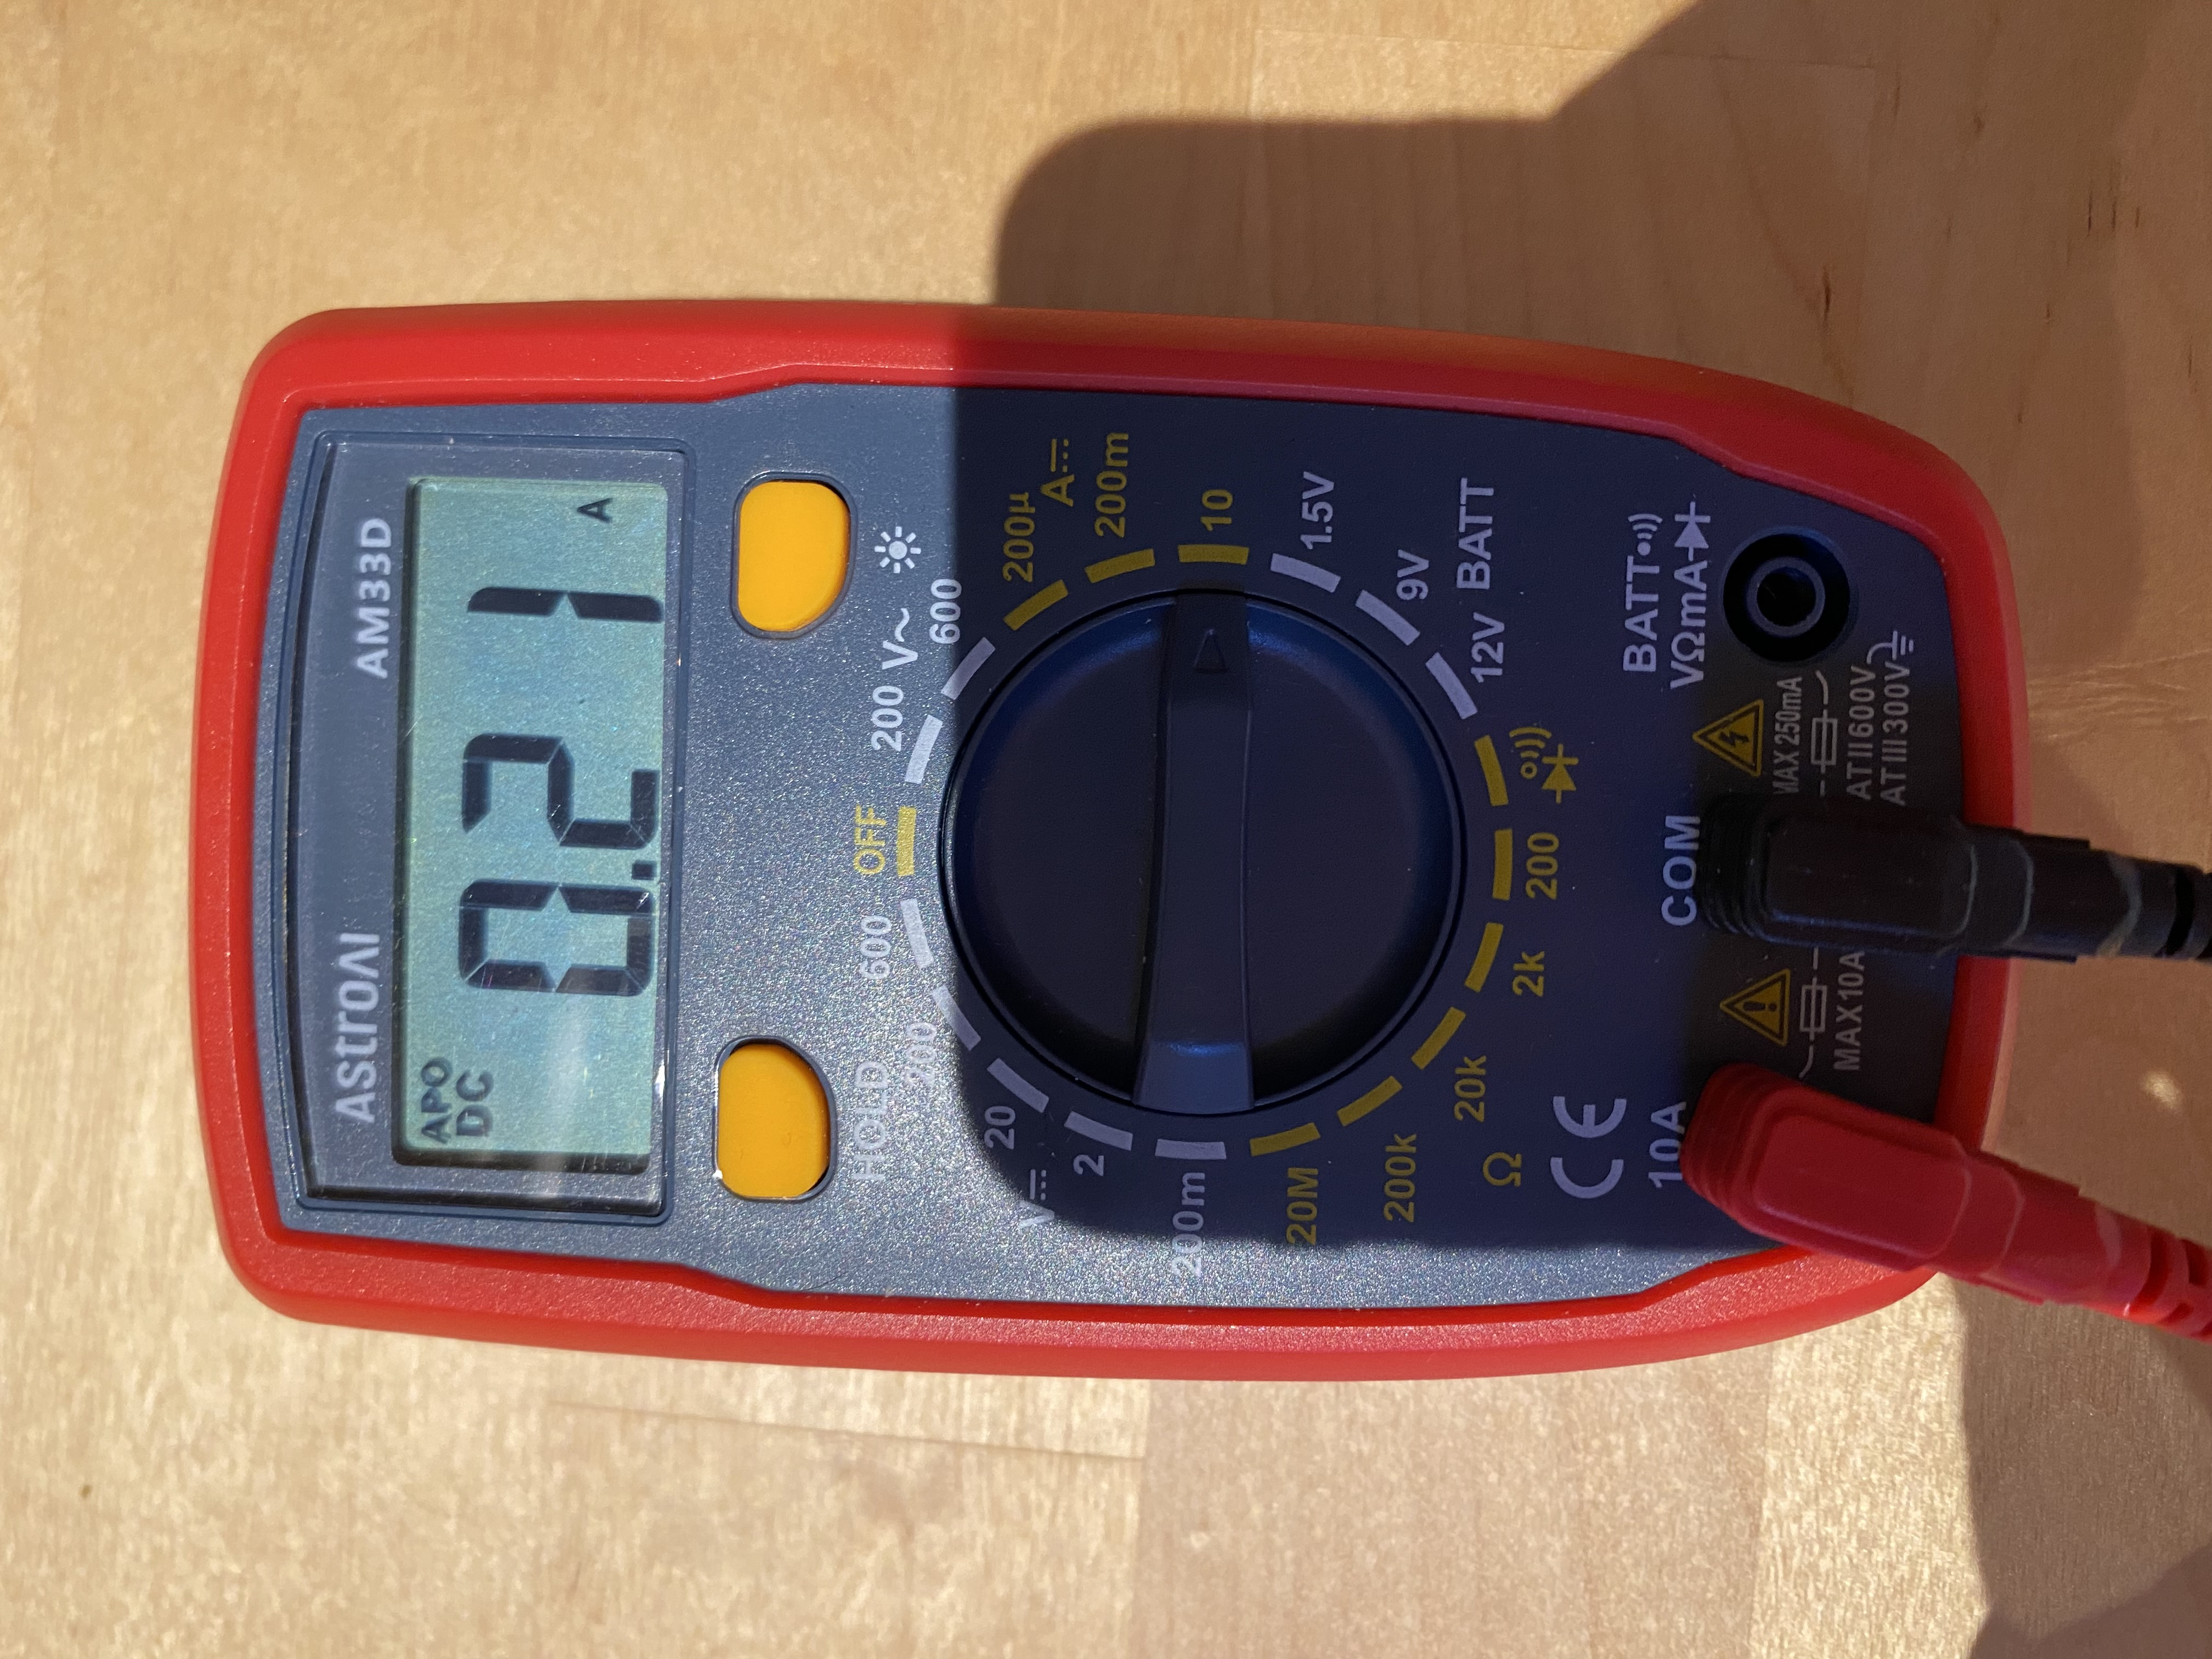
\includegraphics[width=\linewidth,angle=-90]{Figures/multi_21.jpeg}
        \caption{Consumo del sistema en condiciones nominales}
        \label{fig:multi_21}
    \end{subfigure}\hfill
    \begin{subfigure}{0.48\linewidth}
        \centering
        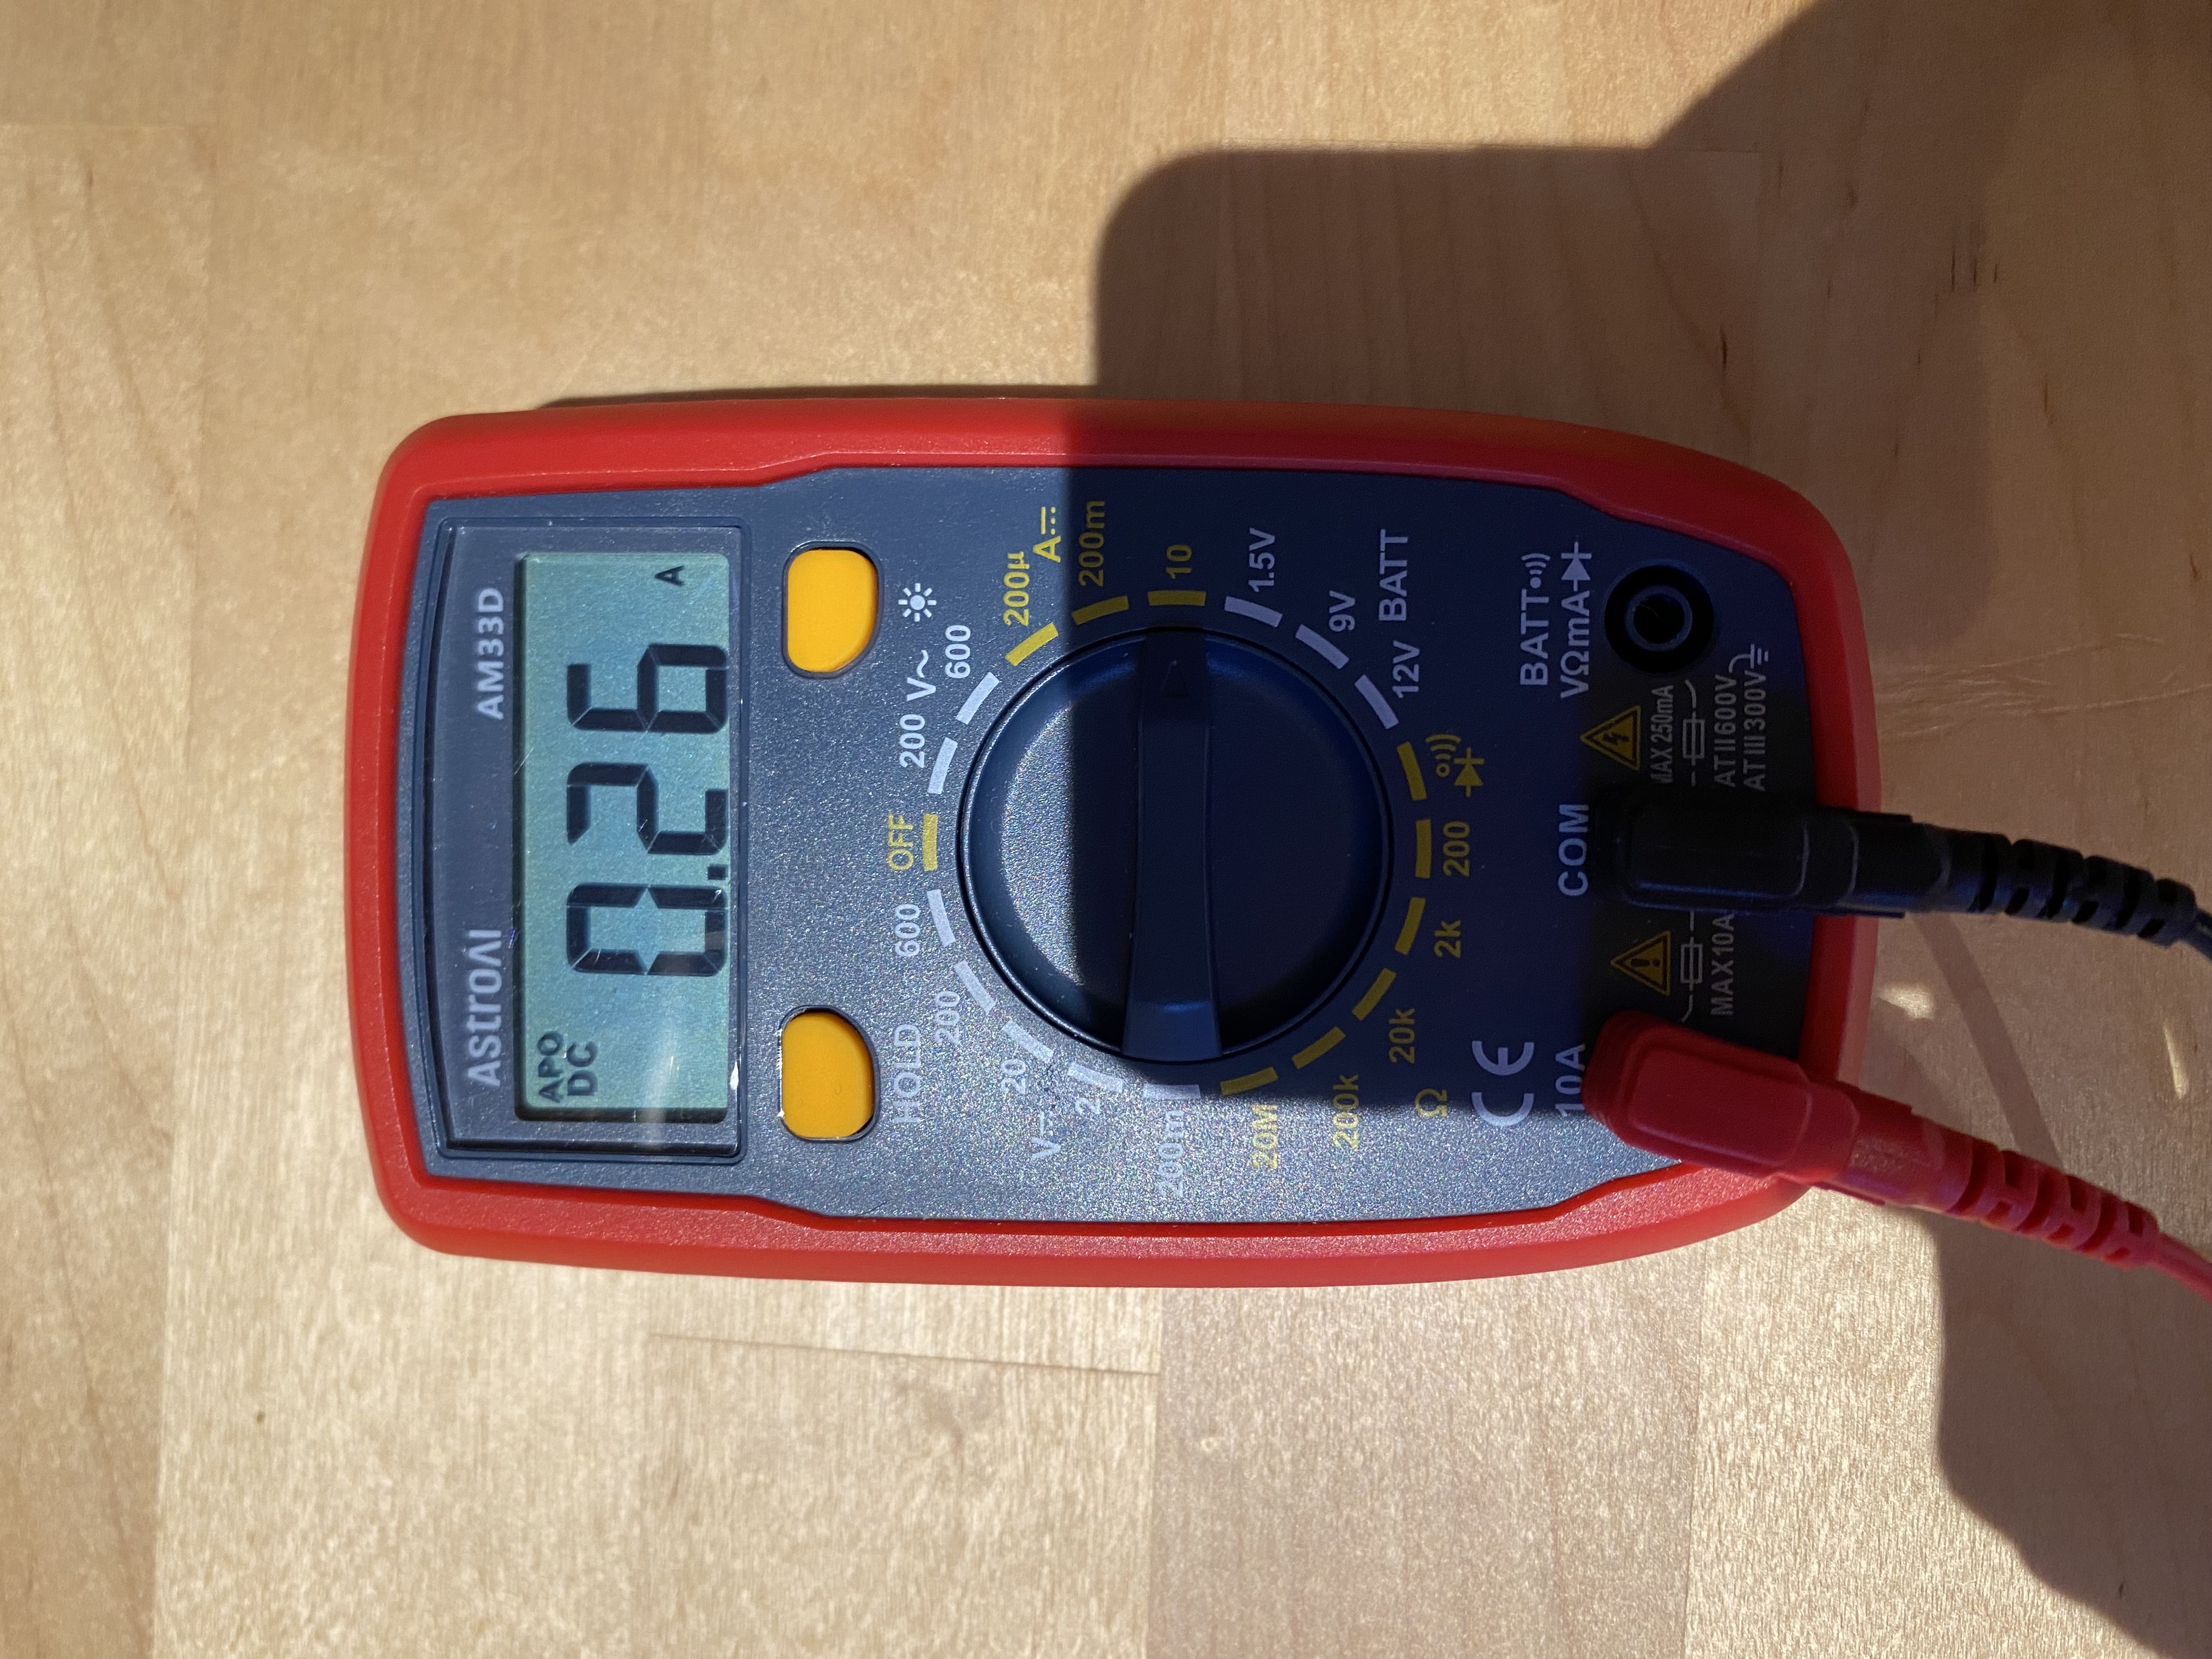
\includegraphics[width=\linewidth,angle=-90]{Figures/multi_26.jpeg}
        \caption{Consumo del sistema sin enlace de telemetría}
        \label{fig:multi_26}
    \end{subfigure}
    \caption{Consumo total del sistema medido con multímetro en serie con la
             alimentación USB-C: condiciones nominales y con el receptor
             desconectado.}
    \label{fig:val_consumo}
\end{figure}

\subsection{Integridad del bus I2C}
\label{sec:val_i2c}

Para verificar el bus I2C compartido por los tres sensores (MPU-9250, BMP280 y
VL53L1X) se capturan simultáneamente las líneas de reloj (SCL) y de datos (SDA)
durante el funcionamiento normal (\cref{fig:val_i2c}). El reloj presenta una
frecuencia de \SI{400}{\kilo\hertz}, coincidiendo con el valor configurado en la
\cref{sec:fw_imu}, y el bus opera de forma estable durante todo el funcionamiento,
sin pérdida de tramas ni errores de lectura de los sensores. Esto confirma en
operación lo indicado en la \cref{sec:bus_i2c}: el valor
equivalente de las resistencias de pull-up de los módulos es adecuado y el bus
opera sin problemas a la velocidad configurada.

\begin{figure}[H]
    \centering
    \includegraphics[width=0.7\linewidth]{Figures/png/DSO00014.png}
    \caption{Líneas SCL y SDA del bus I2C a \SI{400}{\kilo\hertz}.}
    \label{fig:val_i2c}
\end{figure}


% ========================================================================
\section{Validación funcional}
\label{sec:val_funcional}

Con el sistema completo integrado y en funcionamiento se comprueba que cada
requisito funcional queda cubierto. El nodo transmisor adquiere y fusiona los
datos, los codifica en ARINC 429 y los transmite. El receptor los decodifica y
los entrega al PC y el PFD los representa en disposición Basic-T. 

La \cref{tab:val_funcional} resume la comprobación de cada requisito funcional.

\begin{table}[H]
    \centering
    \caption{Comprobación de los requisitos funcionales}
    \label{tab:val_funcional}
    \footnotesize
    \begin{tabularx}{\linewidth}{l X l}
        \toprule
        \textbf{ID} & \textbf{Comprobación} & \textbf{Estado} \\
        \midrule
        RF01 & El horizonte artificial sigue el cabeceo y el alabeo de la placa en tiempo real. & Cumple \\
        RF02 & El indicador de rumbo refleja el rumbo magnético; precisión cuantificada en la \cref{sec:val_rumbo}. & Cumple \\
        RF03 & La cinta de altitud muestra la altitud MSL derivada de la presión barométrica. & Cumple \\
        RF04 & El VSI muestra la velocidad vertical estimada. & Cumple \\
        RF05 & La cinta de velocidad muestra la velocidad respecto al suelo del GNSS cuando hay \textit{fix}. & Cumple \\
        RF06 & El indicador de proximidad muestra la distancia al suelo (ToF como fuente activa). & Cumple \\
        RF07 & La telemetría llega del transmisor al receptor; enlace validado en la \cref{sec:val_enlace}. & Cumple \\
        RF08 & El receptor decodifica las palabras ARINC 429 por etiqueta y descarta las inválidas. & Cumple \\
        RF09 & El PFD se representa con la disposición Basic-T completa. & Cumple \\
        \bottomrule
    \end{tabularx}
\end{table}


% ========================================================================
\section{Precisión de la estimación de actitud}
\label{sec:val_actitud}

Para estudiar la precisión de la estimación de actitud, se evalúa esta magnitud en condiciones estáticas frente a ángulos de referencia conocidos. Para obtener estos ángulos se emplean escuadras de dibujo apoyadas sobre una superficie plana y nivelada, con las que se fijan las referencias de $30^{\circ}$, $45^{\circ}$ y $60^{\circ}$. Para cada ángulo se registra el valor de cabeceo (P) o alabeo (R) indicado por el PFD. Antes de tomar las medidas se han aplicado los \textit{offsets} de montaje de la \cref{tab:mahony_params}.

El montaje empleado se muestra en la \cref{fig:val_actitud_escuadra} y los valores obtenidos se recogen en la \cref{tab:val_actitud} (El resto de imagenes de las pruebas se encuentran en el Anexo III). El error máximo observado es de $1{,}8^{\circ}$, dentro del umbral de $3^{\circ}$ fijado por RP04.

\begin{table}[H]
    \centering
    \caption{Precisión de la estimación de actitud en condiciones estáticas}
    \label{tab:val_actitud}
    \footnotesize
    \begin{tabularx}{\linewidth}{C{2.6cm} C{2.4cm} C{2.0cm} C{2.4cm} C{2.0cm}}
        \toprule
        \textbf{Ref.\ ($^{\circ}$)} & \textbf{Cabeceo P ($^{\circ}$)} & \textbf{Error ($^{\circ}$)} & \textbf{Alabeo R ($^{\circ}$)} & \textbf{Error ($^{\circ}$)} \\
        \midrule
        $0$    & $-0{,}1$  & $0{,}1$ & $0{,}1$   & $0{,}1$ \\
        $+30$  & $28{,}9$  & $1{,}1$ & $29{,}1$  & $0{,}9$ \\
        $-30$  & $-29{,}9$ & $0{,}1$ & $-29{,}3$ & $0{,}7$ \\
        $+45$  & $43{,}4$  & $1{,}6$ & $43{,}8$  & $1{,}2$ \\
        $-45$  & $-44{,}4$ & $0{,}6$ & $-43{,}8$ & $1{,}2$ \\
        $+60$  & $58{,}2$  & $1{,}8$ & $58{,}5$  & $1{,}5$ \\
        $-60$  & $-59{,}1$ & $0{,}9$ & $-58{,}8$ & $1{,}2$ \\
        \bottomrule
    \end{tabularx}
\end{table}

\begin{figure}[H]
    \centering
    
    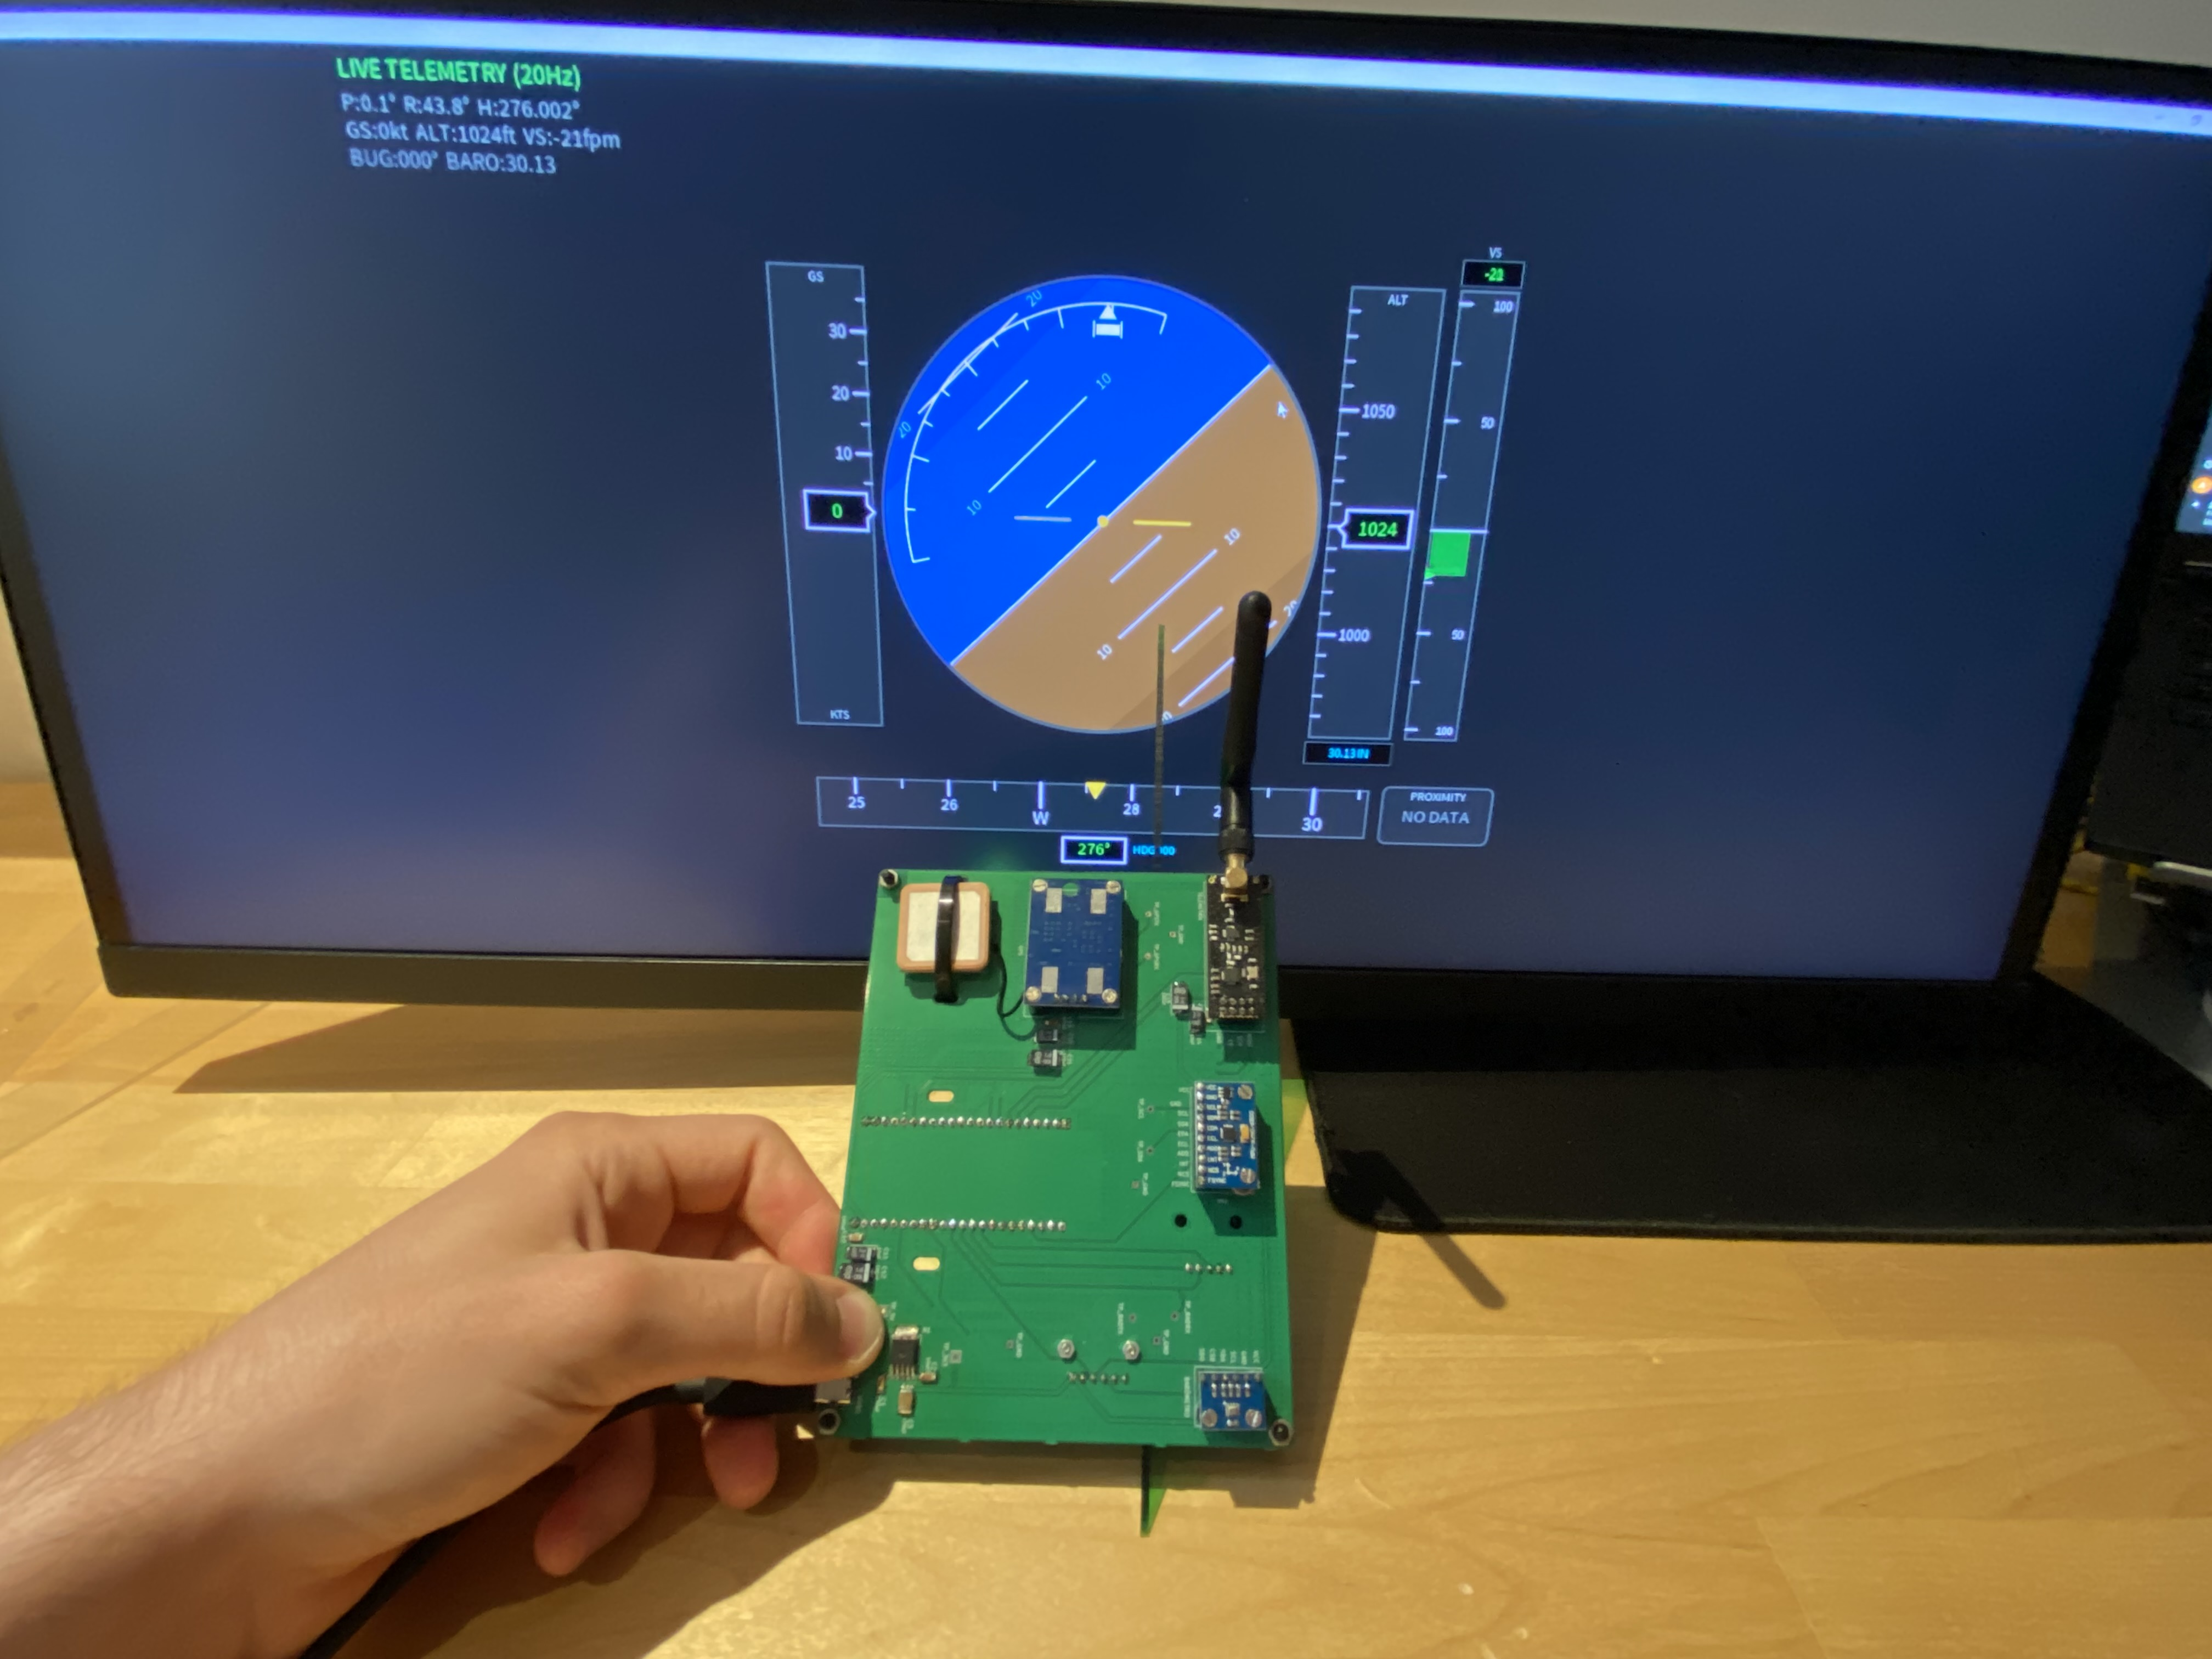
\includegraphics[width=0.6\linewidth]{Figures/IMG_2157.jpeg}
    \caption{Montaje para la medida de precisión de actitud con escuadra de
             referencia.}
    \label{fig:val_actitud_escuadra}
\end{figure}


% ========================================================================
\section{Rumbo magnético}
\label{sec:val_rumbo}

El rumbo magnético se valida en interior con la referencia de un teléfono móvil, que incorpora su propia calibración
y fusión, en varias orientaciones repartidas alrededor de los $360^{\circ}$. En cada
orientación se registra el rumbo indicado por la plataforma y el indicado por el
teléfono, y se calcula su desviación (\cref{tab:val_rumbo}).

{
\footnotesize
\begin{longtable}{C{3.2cm} C{3.2cm} C{3.2cm}}
\caption{Comparación del rumbo de la plataforma frente a un teléfono móvil}
\label{tab:val_rumbo} \\

\toprule
\textbf{Plataforma ($^{\circ}$)} & \textbf{Teléfono ($^{\circ}$)} & \textbf{Desviación ($^{\circ}$)} \\
\midrule
\endfirsthead

% Encabezado para la segunda página (y siguientes)
\multicolumn{3}{c}{\tablename\ \thetable\ -- Continuación de la página anterior} \\
\toprule
\textbf{Plataforma ($^{\circ}$)} & \textbf{Teléfono ($^{\circ}$)} & \textbf{Desviación ($^{\circ}$)} \\
\midrule
\endhead

% Pie de página temporal si la tabla se corta
\midrule
\multicolumn{3}{r}{\textit{Continúa en la siguiente página...}} \\
\endfoot

% Pie de página final para la última página de la tabla
\bottomrule
\endlastfoot

% --- Datos ---
$4{,}5$ & $0$ & $+4{,}5$ \\
$13{,}5$ & $10$ & $+3{,}5$ \\
$23{,}5$ & $20$ & $+3{,}5$ \\
$33{,}5$ & $30$ & $+3{,}5$ \\
$44{,}5$ & $40$ & $+4{,}5$ \\
$53{,}5$ & $50$ & $+3{,}5$ \\
$63{,}5$ & $60$ & $+3{,}5$ \\
$74{,}5$ & $70$ & $+4{,}5$ \\
$83{,}5$ & $80$ & $+3{,}5$ \\
$94{,}5$ & $90$ & $+4{,}5$ \\
$102{,}5$ & $100$ & $+2{,}5$ \\
$112{,}5$ & $110$ & $+2{,}5$ \\
$122{,}5$ & $120$ & $+2{,}5$ \\
$131{,}5$ & $130$ & $+1{,}5$ \\
$141{,}5$ & $140$ & $+1{,}5$ \\
$151{,}5$ & $150$ & $+1{,}5$ \\
$161{,}5$ & $160$ & $+1{,}5$ \\
$170{,}5$ & $170$ & $+0{,}5$ \\
$179{,}5$ & $180$ & $-0{,}5$ \\
$189{,}5$ & $190$ & $-0{,}5$ \\
$199{,}5$ & $200$ & $-0{,}5$ \\
$205{,}5$ & $207$ & $-1{,}5$ \\
$209{,}5$ & $210$ & $-0{,}5$ \\
$219{,}5$ & $220$ & $-0{,}5$ \\
$229{,}5$ & $230$ & $-0{,}5$ \\
$240{,}5$ & $240$ & $+0{,}5$ \\
$249{,}5$ & $250$ & $-0{,}5$ \\
$259{,}5$ & $260$ & $-0{,}5$ \\
$269{,}5$ & $270$ & $-0{,}5$ \\
$280{,}5$ & $280$ & $+0{,}5$ \\
$288{,}5$ & $290$ & $-1{,}5$ \\
$300{,}5$ & $300$ & $+0{,}5$ \\
$309{,}5$ & $310$ & $-0{,}5$ \\
$321{,}5$ & $320$ & $+1{,}5$ \\
$332{,}5$ & $330$ & $+2{,}5$ \\
$341{,}5$ & $340$ & $+1{,}5$ \\
$353{,}5$ & $350$ & $+3{,}5$ \\

\end{longtable}
}

\begin{figure}[H]
    \centering
    \begin{tikzpicture}
    \begin{axis}[
        width=0.85\linewidth, height=6cm,
        xlabel={Rumbo de referencia (tel\'efono) [$^\circ$]},
        ylabel={Desviaci\'on plataforma$-$tel\'efono [$^\circ$]},
        xmin=0, xmax=360, xtick={0,45,90,135,180,225,270,315,360},
        ymin=-3, ymax=6, grid=both, grid style={gray!20},
        tick label style={font=\footnotesize}, label style={font=\footnotesize},
    ]
    \addplot[only marks, mark=*, mark size=1.3pt] coordinates {
        (207,-1.5) (200,-0.5) (190,-0.5) (180,-0.5) (170,0.5) (160,1.5) 
        (150,1.5) (140,1.5) (130,1.5) (120,2.5) (110,2.5) (100,2.5) 
        (90,4.5) (80,3.5) (70,4.5) (60,3.5) (50,3.5) (40,4.5) (30,3.5) 
        (20,3.5) (10,3.5) (0,4.5) (350,3.5) (340,1.5) (330,2.5) 
        (320,1.5) (310,-0.5) (300,0.5) (290,-1.5) (280,0.5) (270,-0.5) 
        (260,-0.5) (250,-0.5) (240,0.5) (230,-0.5) (220,-0.5) (210,-0.5)
    };
    \addplot[dashed, domain=0:360, thick] {1.5};
    \addplot[domain=0:360] {0};
    \end{axis}
    \end{tikzpicture}
    \caption{Desviaci\'on del rumbo de la plataforma frente al tel\'efono. La l\'inea discontinua marca el
             sesgo medio residual ($+1{,}5^\circ$) tras la calibraci\'on.}
    \label{fig:val_rumbo_scatter}
\end{figure}

Estos resultados conviene analizarlos con cautela, ya que en interior existen múltiples interferencias que pueden afectar tanto a la plataforma como al teléfono. Por ello, esta comparación es más una verificación de la consistencia entre ambos magnetómetros que una medida exacta del norte verdadero. Aun así, los valores del teléfono se toman como buena referencia, y las desviaciones de la \cref{fig:val_rumbo_scatter} se mantienen dentro de márgenes aceptables.


% ========================================================================
\section{Precisión del posicionamiento GNSS}
\label{sec:val_gnss}

La precisión del posicionamiento se evalúa dejando la plataforma estática en
exterior, con vista despejada del cielo, y registrando la posición a \SI{5}{\hertz}
durante varios minutos. Sobre el conjunto de fijaciones se calcula la dispersión
respecto al centroide y, a partir de ella, el error circular probable (CEP).

Se obtiene un CEP50 de \SI{1.00}{\meter} y un CEP95 de \SI{1.86}{\meter}
(\cref{fig:val_gnss_scatter}). Ambos valores quedan por debajo del objetivo de
\SI{2.5}{\meter} de CEP fijado por RP05, que toma como referencia la cifra de la
hoja de datos del NEO-6M \cite{ds_neo6}. La retícula que se aprecia en la
distribución corresponde a la cuantización de la posición en la telemetría
(resolución de aproximadamente \SI{0.42}{\meter} por bit, \cref{sec:fw_word}); dado
que la dispersión real de las fijaciones, del orden de \SI{2}{\meter}, es muy
superior a ese paso, la cuantización no condiciona el valor del CEP obtenido.

\begin{figure}[H]
    \centering
    \includegraphics[width=0.7\linewidth]{Figures/val_gnss_scatter.png}
    \caption{Dispersión del posicionamiento GNSS en estático, con los círculos de
             CEP50 (\SI{1.00}{\meter}) y CEP95 (\SI{1.86}{\meter}).}
    \label{fig:val_gnss_scatter}
\end{figure}



% ========================================================================
\section{Precisión del sensor de distancia al suelo}
\label{sec:val_distancia}

La medida de distancia al suelo (RF06) se evalúa frente a distancias de
referencia conocidas, medidas con una cinta métrica. La plataforma se sitúa a
distintas alturas sobre una superficie plana (\SI{10}{\centi\meter},
\SI{20}{\centi\meter}, \SI{50}{\centi\meter} y valores adicionales) y se registra
la distancia indicada por el sensor de tiempo de vuelo VL53L1X, que es la fuente
activa del indicador de proximidad (\cref{sec:fw_proximidad}). La
\cref{tab:val_distancia} recoge las medidas; el error máximo del ToF es de
\SI{1.9}{\centi\meter}, coherente con la precisión de la hoja de datos
\cite{ds_vl53l1x}.

El radar HLK-LD2410C se incluye en la telemetría como segunda fuente, pero su
salida es una clasificación por puertas de distancia, no una medida métrica
estable, por lo que no se contrasta cuantitativamente; su papel es comparativo y
docente, según lo justificado en la \cref{sec:fw_proximidad}.

\begin{table}[H]
    \centering
    \caption{Precisión del sensor de distancia al suelo (VL53L1X)}
    \label{tab:val_distancia}
    \footnotesize
    \begin{tabularx}{\linewidth}{C{4.0cm} C{4.0cm} C{4.0cm}}
        \toprule
        \textbf{Ref.\ (\si{\centi\meter})} & \textbf{ToF medido (\si{\centi\meter})} & \textbf{Error (\si{\centi\meter})} \\
        \midrule
        $10$  & $10{,}3$ & $+0{,}3$ \\
        $20$  & $19{,}5$ & $-0{,}5$ \\
        $50$  & $51{,}2$ & $+1{,}2$ \\
        $100$ & $98{,}1$ & $-1{,}9$ \\
        \bottomrule
    \end{tabularx}
\end{table}


\section{Enlace de telemetría}
\label{sec:val_enlace}

La cobertura del requisito de alcance y fiabilidad del enlace (RP06) se justifica
por margen de diseño. El módulo NRF24L01+PA/LNA seleccionado (\cref{sec:enlace})
presenta un alcance en interior del orden de \SI{100}{\meter}, muy por encima de
las distancias de uso en laboratorio (unos pocos metros, con posibilidad de un
tabique intermedio), por lo que el enlace opera con holgura en el escenario
previsto. Como apoyo a la operación, el receptor emite cada segundo una sentencia
de estadística (\texttt{\$STATS}: paquetes recibidos y un porcentaje de pérdida
estimado a partir de las palabras de estado, a \SI{5}{\hertz}). Se trata de un
indicador de salud del enlace para supervisión en tiempo de ejecución, no de una
medida validada de pérdida de paquetes.


% ========================================================================
\section{Tasas de actualización y latencia}
\label{sec:val_latencia}

\paragraph{Tasa de refresco del PFD (RP02).}
El PFD se redibuja con el motor P2D a \SI{60}{FPS}, valor fijado por configuración
y muy por encima del mínimo de \SI{30}{FPS} de RP02.

\paragraph{Tasa de actualización de actitud (RP03).}
La fusión de actitud se ejecuta a \SI{100}{\hertz} y la actitud se transmite a
\SI{20}{\hertz}; ambas cadencias quedan fijadas por el planificador cooperativo
del firmware y superan el mínimo de \SI{20}{\hertz} de RP03.

\paragraph{Latencia extremo a extremo (RP01).}
La latencia extremo a extremo se acota analíticamente mediante el presupuesto de
retardos de transporte de la cadena, recogido en la \cref{tab:val_latencia}.

\begin{table}[H]
    \centering
    \caption{Presupuesto de latencia extremo a extremo (peor caso)}
    \label{tab:val_latencia}
    \footnotesize
    \begin{tabularx}{\linewidth}{X l}
        \toprule
        \textbf{Etapa} & \textbf{Contribución} \\
        \midrule
        Muestreo inercial y fusión (\SI{100}{\hertz})                 & $\approx$ \SI{10}{\milli\second} \\
        Espera del \textit{slot} de telemetría (\SI{20}{\hertz})       & $\leq$ \SI{50}{\milli\second} \\
        Transmisión RF con reconocimiento (\num{250}~kbps, \SI{32}{\byte}) & $\approx$ \SI{2}{\milli\second} \\
        Decodificación y salida serie USB (\SI{115200}{\baud}, $\approx$\SI{70}{\byte}) & $\approx$ \SI{6}{\milli\second} \\
        Espera de fotograma (\SI{60}{FPS})                            & $\leq$ \SI{17}{\milli\second} \\
        \midrule
        \textbf{Total (peor caso)}                                    & $\approx$ \SI{85}{\milli\second} \\
        \bottomrule
    \end{tabularx}
\end{table}

El peor caso, de aproximadamente \SI{85}{\milli\second}, queda por debajo del
límite de \SI{200}{\milli\second} de RP01. La latencia típica es menor, ya que los
términos de espera (\textit{slot} de telemetría y fotograma) promedian
aproximadamente la mitad de su valor de peor caso. 


% ========================================================================
\section{Resumen de cumplimiento de requisitos}
\label{sec:val_resumen}

La \cref{tab:val_cumplimiento} consolida el resultado de la validación frente a
los requisitos de rendimiento. Los requisitos funcionales (RF01--RF09) quedan
cubiertos según la \cref{tab:val_funcional}.

\begin{table}[H]
    \centering
    \caption{Resumen de cumplimiento de los requisitos de rendimiento}
    \label{tab:val_cumplimiento}
    \footnotesize
    \begin{tabularx}{\linewidth}{l X l l}
        \toprule
        \textbf{ID} & \textbf{Objetivo} & \textbf{Resultado} & \textbf{Estado} \\
        \midrule
        RP01 & Latencia $<$ \SI{200}{\milli\second}            & $\approx$ \SI{85}{\milli\second}  & Cumple \\
        RP02 & Refresco PFD $\geq$ \SI{30}{FPS}                & \SI{60}{FPS}            & Cumple \\
        RP03 & Actitud $\geq$ \SI{20}{\hertz}                  & \SI{20}{\hertz}  & Cumple \\
        RP04 & Actitud $\pm 3^{\circ}$                & error máx.\ $1{,}8^{\circ}$ & Cumple \\
        RP05 & GNSS $\leq$ \SI{2.5}{\meter} CEP                & \SI{1.00}{\meter} CEP50 & Cumple \\
        RP06 & Alcance de decenas de metros en interior        & $\approx$ \SI{100}{\meter} & Cumple \\
        \bottomrule
    \end{tabularx}
\end{table}
\cleardoublepage

% Capítulo 9: Presupuesto
%!TEX root = ../main.tex

\chapter{Presupuesto}
\label{ch:presupuesto}

Este capítulo ofrece un resumen del coste del desarrollo de la plataforma experimental. Para el desglose total, este se detalla en el documento de Presupuesto entregado de forma independiente.

\section{Resumen económico}
\label{sec:resumen_economico}

El coste se desglosa en las siguientes categorías: materiales, amortización de los equipos de laboratorio
empleados, software y coste de personal. En la \cref{tab:resumen_economico} se recoge el
coste total dividido en categorías. El coste total del proyecto asciende a \SI{14547.32}{\eur} con IVA incluido.

\begin{table}[H]
    \centering
    \caption{Resumen del coste del proyecto}
    \label{tab:resumen_economico}
    \footnotesize
    \begin{tabularx}{\linewidth}{X r}
        \toprule
        \textbf{Concepto} & \textbf{Coste} \\
        \midrule
        Materiales              & \SI{92}{\eur} \\
        Amortización de equipos & \SI{37.62}{\eur} \\
        Software                & \SI{0}{\eur} \\
        Personal                & \SI{10800}{\eur} \\
        \midrule
        Total (con costes indirectos del \SI{10}{\percent} e IVA del \SI{21}{\percent}) & \SI{14547.32}{\eur} \\
        \bottomrule
    \end{tabularx}
\end{table}
\cleardoublepage

% Capítulo 10: Análisis de sostenibilidad e implicaciones
%!TEX root = ../main.tex

\chapter{Análisis de sostenibilidad e implicaciones}
\label{ch:impacto}

\section{Impacto ambiental}
\label{sec:impacto_ambiental}

La mayor parte del impacto ambiental del sistema proviene de los componentes electrónicos, los módulos comerciales y la placa de circuito impreso. Al ser un equipo único, su huella de fabricación es pequeña, pero le afectan los mismos factores que a cualquier componente electrónico. Por un lado, los materiales usados están sujetos a la normativa RoHS \cite{dir_rohs}, la cual limita el uso de sustancias como el plomo o el mercurio. Por otro lado, al final de su vida útil, el conjunto debe ser gestionado como residuo de aparato eléctrico y electrónico (RAEE) \cite{dir_raee}, requiriendo un reciclaje separado de la basura común.

En el ámbito de su alimentación y consumo, el gasto del sistema en funcionamiento es muy bajo, ofreciendo un impacto mínimo en este aspecto. Al alimentarse por USB-C y no incluir baterías, tampoco genera residuos asociados con las celdas de litio u otros materiales presentes en ellas.

Por último, el hecho de que el software sea de código abierto ayuda a alargar la vida del producto, ya que cualquiera puede repararlo, modificarlo o reutilizarlo, reduciendo así la obsolescencia y evitando su desecho antes de tiempo.
\cleardoublepage

% Capítulo 11: Conclusiones y Trabajo Futuro
%!TEX root = ../main.tex

\chapter{Conclusiones y trabajo futuro}
\label{ch:conclusiones}

\section{Conclusiones}
\label{sec:conclusiones}

El objetivo principal del proyecto, el diseño y la implementación de una plataforma experimental de bajo coste para la emulación de instrumentación aviónica, se ha logrado satisfactoriamente. Se han creado los tres subsistemas planteados en la \cref{sec:objetivo}: una placa de circuito impreso que integra el microcontrolador y los sensores, un firmware que adquiere, calibra, fusiona y transmite los datos, y un Primary Flight Display desarrollado en Processing con la disposición Basic-T. Estos tres subsistemas han sido integrados y operan como un único sistema, tal y como se documenta en el \cref{ch:validacion}.

Basado en los requisitos definidos, se extraen las siguientes conclusiones:

\begin{itemize}
    \item La fusión sensorial mediante el filtro Mahony MARG proporciona una estimación de actitud y rumbo estable en tiempo real. 

    \item Reutilizar la capa lógica del estándar ARINC 429 sobre el enlace de radio permite estructurar la telemetría acorde a la práctica aeronáutica. El planificador por etiqueta encaja con la restricción de carga útil del transceptor, como se describe en el \cref{ch:firmware}.

    \item La selección de componentes, orientada al valor didáctico, ofrece al estudiante acceso a las magnitudes intermedias del sistema y a los algoritmos subyacentes.

    \item El PFD reproduce la disposición Basic-T marcada por la regulación y representa en tiempo real los parámetros calculados, cerrando la cadena desde el sensor hasta la pantalla.
\end{itemize}

En conjunto, la plataforma cumple su propósito. Permite recorrer toda la cadena de instrumentación aviónica, es de código abierto y se puede replicar por menos de \SI{100}{\eur} en materiales, lo que la hace adecuada para su uso en laboratorios docentes. Por otro lado, el sistema no incorpora la redundancia ni los mecanismos de seguridad requeridos en un equipo de vuelo, y la exactitud del rumbo en interiores queda limitada por el entorno magnético, como se analiza en la \cref{sec:val_rumbo}.


\section{Trabajo futuro}
\label{sec:trabajo_futuro}

A partir de las actividades excluidas en la \cref{sec:exclusiones} y de las limitaciones identificadas, se proponen las siguientes líneas de continuación:

\begin{itemize}
    \item \textbf{Ampliación de la vista cartográfica.} La vista de mapa de navegación (\cref{sec:sw_mapa}) emplea teselas descargadas previamente en disco. El siguiente paso sería descargar las teselas en línea bajo demanda y cubrir más niveles de zoom.

    \item \textbf{Integración en una plataforma de vuelo.} Adaptar el sistema para instalarlo en un vehículo aéreo, con todas las implicaciones de certificación y robustez que esto supondría.

    \item \textbf{Representación del Flight Path Vector.} Incluirlo enriquecería el PFD, pero requiere datos adicionales de viento y de parámetros de navegación.

    \item \textbf{Sistemas aviónicos adicionales.} La arquitectura del sistema permitiría incorporar funciones adicionales como radar meteorológico, TCAS, ADS-B o FMS.
\end{itemize}
\cleardoublepage

% Capítulo 12: Declaración de uso de IA generativa
%!TEX root = ../main.tex

\chapter{Declaración sobre el uso de herramientas de inteligencia artificial}
\label{ch:decl_ia}

Cumpliendo con la nueva normativa de la ESEIAAT sobre el uso de herramientas de inteligencia artificial en trabajos de fin de estudios, se declara que en este trabajo se ha hecho uso de estas herramientas durante la elaboración. La herramienta utilizada ha sido:

\begin{itemize}
    \item Claude (Anthropic).
\end{itemize}

El uso principal ha sido la revisión ortográfica, gramatical y de estilo del texto de la memoria del proyecto, la corrección de erratas y el apoyo en la estructuración del documento. También se ha utilizado para consultas puntuales de formato del documento (\LaTeX), como algún diagrama. Esta asistencia ha estado presente en la globalidad del documento. Por lo que respecta al contenido técnico (el diseño del hardware y de la placa, el desarrollo del firmware, la implementación del PFD, las decisiones de diseño y los resultados experimentales), es obra del autor en su mayoría. En algunas partes del código se ha hecho uso de esta herramienta para aclarar conceptos o escribir alguna parte menor.

Todo el contenido generado por la herramienta ha sido revisado, verificado y editado en mayor o menor medida por el autor antes de su incorporación al trabajo, descartando o corrigiendo aquello que no se ajustaba al mismo o que se consideraba no apto. El autor asume la responsabilidad sobre la veracidad, integridad y corrección de todo el material contenido en este trabajo.
\cleardoublepage

%%%%%%%%%%%%%%%%%%%%%%%%%%%%%%%%%%%%%%%%%%%%%%%%%%%%%%%%%%%%%%%%%%%%%%%%%%
%                            BIBLIOGRAFÍA                                
%%%%%%%%%%%%%%%%%%%%%%%%%%%%%%%%%%%%%%%%%%%%%%%%%%%%%%%%%%%%%%%%%%%%%%%%%%

% OJO: \nocite{*} imprime TODAS las entradas del .bib aunque no las cites
% (anade ~26 referencias no citadas). Se deja comentado para que la
% bibliografia solo liste lo que citas de verdad. Descomentar solo si el
% tribunal quiere una lista completa de obras consultadas.
%\nocite{*}
\printbibliography[heading=bibnumbered, title={Referencias}]
\cleardoublepage

%%%%%%%%%%%%%%%%%%%%%%%%%%%%%%%%%%%%%%%%%%%%%%%%%%%%%%%%%%%%%%%%%%%%%%%%%%
%                              APÉNDICES                                 
%%%%%%%%%%%%%%%%%%%%%%%%%%%%%%%%%%%%%%%%%%%%%%%%%%%%%%%%%%%%%%%%%%%%%%%%%%

\appendix

% Sin apendices dentro de la memoria: el codigo (anexos) se entrega como
% documento independiente, en la carpeta Anexos con su propio main.tex.

\end{document}